\documentclass[11pt,a4paper,hyphens]{report}
\usepackage{color}
\usepackage{caption}
\usepackage{translit}
\usepackage{amsmath}
% dasselbe Template wie Thesis mit nur leichten Anpassungen
% Nehmen Sie das Thesis-Template für die Thesis!
% Lesen Sie Hinweise zum Umgang mit LaTeX und zum Schreiben
% von Berichten im Thesis-Template nach
% => Moodle => PraxissemesterThesis => LaTeXThesis.zip
%    https://moodle.hs-mannheim.de/course/view.php?id=2500


% Für doppelseitigen Ausdruck (nur bei > 60 Seiten sinnvoll)
% \usepackage{ifthen}
% \setboolean{@twoside}{true}
% \setboolean{@openright}{true} 

% pakete
\usepackage{ifthen}

% Deutsch
\usepackage[german]{babel} % deutsch und deutsche Rechtschreibung
\usepackage[backend=biber, style=numeric, sorting=none]{biblatex} % Literaturverzeichnis (sortiert nach Reihenfolge des Auftretens)
\addbibresource{praksem.bib}
\usepackage[utf8]{inputenc} % Unicode Text
\usepackage[T1]{fontenc} % Umlaute und deutsches Trennen
\usepackage{textcomp} % Euro
\input{hyphenations} % eigene Hyphenations, die für das Dokument gelten
\usepackage{amssymb} % Symbole
\usepackage{emptypage} % Wirklich leer bei leeren Seiten

%% Fonts, je ein kompletter Satz an Optionen

% Times New Roman, gewohnter Font, ok tt und serifenlos
%\usepackage{mathptmx} 
%\usepackage[scaled=.95]{helvet}
%\usepackage{courier}

% Palatino mit guten Fonts für tt und serifenlos
\usepackage{mathpazo} % Palatino, mal was anderes
\usepackage[scaled=.95]{helvet}
\usepackage{courier}

% New Century Schoolbook sieht auch nett aus (macht auch tt und serifenlos)
%\usepackage{newcent}

% Oder default serifenlos mit Helvetica 
% ich kann es nicht mehr sehen ...
%\renewcommand{\familydefault}{\sfdefault}

% ein bisschen eine bessere Verteilung der Buchstaben...
\usepackage{microtype}

% Bilder und Listings
\usepackage{graphicx} % wir wollen Bilder einfügen
\usepackage{subfig} % Teilbilder
\usepackage{wrapfig} % vielleicht doch besser vermeiden
\usepackage{listings} % schöne Quellcode-Listings
% ein paar Einstellungen für akzeptable Listings
\lstset{basicstyle=\ttfamily, columns=[l]flexible, mathescape=true, showstringspaces=false, numbers=left, numberstyle=\tiny}
\lstset{language=python} % und nur schöne Programmiersprachen ;-)
% und eine eigene Umgebung für Listings
\usepackage{float}
\newfloat{listing}{htbp}{scl}[chapter]
\floatname{listing}{Listing}
\usepackage{enumitem} % für bessere Listen
\usepackage{seqsplit} % für den automatischen Zeilenumbruch von langen Zeichenketten

% Seitenlayout
\newcommand{\seitenseitenabstand}{22mm} % 30mm
\usepackage[paper=a4paper,left=\seitenseitenabstand,right=\seitenseitenabstand,height=23cm]{geometry}
\usepackage{setspace}
% \linespread{1.15}
\linespread{1.1}
\setlength{\parskip}{0.5em}
\setlength{\parindent}{0em} % im Deutschen Einrückung nicht üblich, leider

% Seitenmarkierungen 
\newcommand{\phv}{\fontfamily{phv}\fontseries{m}\fontsize{9}{11}\selectfont}
\usepackage{fancyhdr}
\pagestyle{fancy}
\fancyhf{} % initialize: clear all header and footer fields
\fancyhead[L]{\phv Yan Wittmann}
\fancyhead[C]{\phv Bericht zum praktischen Studiensemester}
\fancyhead[R]{\phv \thepage} % page number on the right
\renewcommand{\headrulewidth}{0.4pt} % line under the header
\fancyfoot{} % clears the footer

% Include subsubsections in the Table of Contents
% -1 for part
%  0 for chapter (only in report and book document classes)
%  1 for section
%  2 for subsection
%  3 for subsubsection
%  4 for paragraph
%  5 for subparagraph
\setcounter{tocdepth}{3}

% Theorem-Umgebungen
\newtheorem{definition}{Definition}[chapter]
\newtheorem{satz}{Satz}[chapter]
\newtheorem{lemma}[satz]{Lemma} % gleicher Zähler wie Satz
\newtheorem{theorem}{Theorem}[chapter]
\newenvironment{beweis}[1][Beweis]{\begin{trivlist}
                                       \item[\hskip \labelsep {\textit{#1 }}]}{
\end{trivlist}}
\newcommand{\qed}{\hfill \ensuremath{\square}}

%% Quellen
% Eine Alternative wäre Quellen in Literatur und Online-Quellen
% zu teilen
% \usepackage{bibtopic} 

% Hochschule Logo, noch nicht perfekt
\usepackage{hsmalogo}

% Spezialpakete
\usepackage{epigraph}
\setlength{\epigraphrule}{0pt} % kein Trennstrich

% damit wir nicht so viel tippen müssen, nur für Demo 
% \usepackage{blindtext}

% ifthen für sperrvermerk
\newif\ifsperrvermerk

% klickbare links im inhaltsverzeichnis
\usepackage{hyperref}
\hypersetup{
    colorlinks,
    citecolor=black,
    filecolor=black,
    linkcolor=black,
    urlcolor=black
}

% text shortcut variablen
\newcommand{{\metaeffekt}}{\{met\ae ffekt\}}
\newcommand{\bitkom}{bitkom}
\newcommand{\aeclientZEZESE}{Thales}
\newcommand{\headerand}{und\ }
% weekdays
\newcommand{\weekdayMondayLong}{Mo} % Mo, Montag
\newcommand{\weekdayTuesdayLong}{Di} % Di, Dienstag
\newcommand{\weekdayWednesdayLong}{Mi} % Mi, Mittwoch
\newcommand{\weekdayThursdayLong}{Do} % Do, Donnerstag
\newcommand{\weekdayFridayLong}{Fr} % Fr, Freitag
\newcommand{\weekdaySaturdayLong}{Sa} % Sa, Samstag
\newcommand{\weekdaySundayLong}{So} % So, Sonntag
\newcommand{\weekdayMondayShort}{Mo}
\newcommand{\weekdayTuesdayShort}{Di}
\newcommand{\weekdayWednesdayShort}{Mi}
\newcommand{\weekdayThursdayShort}{Do}
\newcommand{\weekdayFridayShort}{Fr}
\newcommand{\weekdaySaturdayShort}{Sa}
\newcommand{\weekdaySundayShort}{So}

% custom commands
\newcommand{\lweekdaymarginpar}[1]{%
    \marginpar{\raisebox{-1.6em}{\underline{#1}}}
}
\newcommand{\sweekdaymarginpar}[1]{%
    \marginpar{\raisebox{-1.92em}{\underline{#1}}}
}
\newcommand{\qt}[1]{„#1“}

\definecolor{codegray}{gray}{0.9}
\newcommand{\code}[1]{\colorbox{codegray}{\texttt{\detokenize{#1}}}}
\newcommand{\codendt}[1]{\colorbox{codegray}{\texttt{#1}}}

% conditional commands
\newcommand{\includeReport}[2]{
    \ifshortenedReport
    \input{#1} % Inkludiert den ersten Parameter, wenn shortenedReport wahr ist
    \else
    \input{#2} % Inkludiert den zweiten Parameter, wenn shortenedReport falsch ist
    \fi
}

% custom environments
\newenvironment{smitemize}
{ \begin{itemize}
      \setlength{\itemsep}{0em}
      \setlength{\topsep}{0em}
      \setlength{\partopsep}{0em} }
      {
\end{itemize} }

% code listings
\input{latex-listings-powershell/src/latex-listings-powershell}
\definecolor{lst-gray}{rgb}{0.98,0.98,0.98}
\definecolor{lst-blue}{RGB}{40,0.0,255}
\definecolor{lst-green}{RGB}{65,128,95}
\definecolor{lst-red}{RGB}{200,0,85}
\lstset{
    commentstyle=\color{lst-green},
    basicstyle=\small\ttfamily,
    backgroundcolor=\color{lst-gray},
    breaklines=true,
    captionpos=b,
    columns=fixed,
    extendedchars=true,
    frame=single,
    framesep=2pt,
    keepspaces=true,
    keywordstyle=\color{lst-blue},
    language={PowerShell},
    numbers=left,
    numberstyle=\small\ttfamily,
    showstringspaces=false,
    stringstyle=\color{lst-red},
    tabsize=2,
}
 % alle Pakete und Einstellungen

% Hier anpassen 
\newcommand{\autor}{Yan Wittmann}
\newcommand{\matrikelnummer}{2121578}
\newcommand{\fachsemester}{5IB} % im wie vielten Semester waren Sie?
%\newcommand{\studiengang}{Medizintechnik}
%\newcommand{\studiengang}{Technische Informatik}
\newcommand{\studiengang}{Informationstechnik}
\newcommand{\firma}{\metaeffekt\ GmbH}
\newcommand{\standort}{Heidelberg}
\newcommand{\abteilung}{Automated Vulnerability Monitoring}
\newcommand{\betreuer}{Karsten Klein}
\newcommand{\pbeginn}{01.09.2023}
\newcommand{\pende}{29.02.2024}
\newcommand{\tage}{124} % arbeitstagerechner verwenden!
\newcommand{\titel}{Bericht zum praktischen Studiensemester}
\newcommand{\kurztitel}{Praxisbericht}
% \sperrvermerktrue % Kommentar am Anfang der Zeile löschen für Sperrvermerk

% entweder der vollständige oder der gekürzte Bericht
\newif\ifshortenedReport
\shortenedReporttrue

% Wenn jemand unbedingt ein Glossar will, die nächsten drei Zeilen...
%\usepackage{glossaries} % oder schlimmer mit [toc], damit es im TOC auftaucht
%\makeglossaries
%\input{glossar} % In dieser Datei die Einträge definieren
% und noch ganz unten printglossaries auskommentieren
% Damit jetzt ein Glossar gezeigt wird noch \gls{label} verwenden

\begin{document}
    \include{vorspann} % Titelseite, Erklärungen, etc.

    \begin{abstract}

        Im Rahmen des praktischen Studiensemesters bei der {metæffekt} GmbH in Heidelberg, fokussierte sich Yan Wittmann auf die Weiterentwicklung und Optimierung des automatisierten Vulnerability Monitorings.
        Durch die Einarbeitung in den neuen CVSS 4.0 Standard, die Überarbeitung des Datenmodells und die Implementierung eines TypeScript CVSS Calculators, trug Wittmann zur Verbesserung der Softwarelösungen bei.
        Zusätzlich wurden die Ergebnisse in Kundenprojekten integriert und ein Beitrag zur Open-Source-Community geleistet.

    \end{abstract}

    \tableofcontents

    \ifshortenedReport
    \vspace*{20px}
    \fbox{
        \begin{minipage}{1\textwidth}
            \textbf{Hinweis:}
            Dieser Bericht wurde aus Gründen der Übersichtlichkeit und der maximalen Seitenzahl gekürzt.
            Der vollständige Bericht ist alternativ auf Anfrage verfügbar.
        \end{minipage}
    }
    \fi


    %! Author = Yan Wittmann


\chapter{Einleitung} \label{ch:einleitung}


\section{Firma} \label{sec:firma-beschreibung}

Die {\metaeffekt} GmbH ist ein spezialisiertes Unternehmen, das sich auf die kontinuierliche Inventarisierung, Dokumentation und Bewertung von Risiken in Softwarebestandteilen von Produkten und Projekten konzentriert, um Unternehmen bei der Software Composition Analysis zu unterstützen.
Das Unternehmen arbeitet eng mit verschiedenen Fachbereichen und Verantwortlichen zusammen, um maßgeschneiderte Lösungen anzubieten.
Darüber hinaus bietet die {\metaeffekt} Schulungen und Seminare zu Themen wie License Compliance Awareness, License Compliance Management, Vulnerability Monitoring und Vulnerability Assessment.

Die {\metaeffekt} hebt sich durch einen Fokus auf die tatsächlich genutzten Softwarebestandteile im Gegensatz zu einem spezifikationsbasierten Scannen von anderen Tools und Unternehmen ab.
Durch den Einsatz fallspezifischer Werkzeuge und Beratung erreicht das Unternehmen eine hohe Datenqualität, die für die Umsetzung der License Compliance in der Lieferkette und für die Identifikation sowie Überwachung von öffentlichen Schwachstellen wichtig ist.

Die Abteilung \qt{Vulnerability Monitoring}, in der das Praktikum stattfand, entwickelt Tooling und Prozesse, um die automatisierte kontinuierliche Überwachung von Schwachstellen in Softwareprodukten durch die erfassten Software-Inventare zu ermöglichen.

Es gibt mehrere andere Organisationen, die Teile der Dienstleistungen von {\metaeffekt} anbieten.
Dazu gehören Unternehmen wie
Black Duck (Sicherheits- und Lizenzanforderungsanalyse von Open Source-Komponenten),
WhiteSource (Lizenzanforderungsanalyse von Open Source-Komponenten und Compliance),
Snyk (Identifizierung und Behebung von Sicherheitslücken in Open Source-Komponenten) und
Sonatype (Identifizierung und Behebung von Sicherheitslücken und Lizenzproblemen in Open Source-Komponenten).


\section{Zielsetzung} \label{sec:zielsetzung-des-praktikums}

Das Ziel meines Praktikums war es vor allem, die von mir zuvor entwickelte Softwarelösung für die automatisierte Überwachung von Schwachstellen in Softwareprodukten bei den Kunden zu betreuen, zu verbessern und zu erweitern.
Spezifische Ziele haben sich während den ersten Wochen herausgebildet.

Das erste Ziel sollte das Ersetzen der bisherigen \qt{Generation 2} unseres Vulnerability Monitoring durch eine \qt{Generation 3} sein.
Dies beinhaltet nicht nur die Implementierung des Standards CVSS in der Version 4.0 in Java, sondern auch eine komplette Überarbeitung unseres Datenmodells hinter dem Schwachstellen-Management und die Integration all dieser Änderungen in unsere Systeme und Reports, aufgrund von Erkenntnissen, die über die letzten Monate entstanden sind.

Das zweite Ziel war es, eine TypeScript-Implementierung aller aktuellen CVSS-Versionen zu schreiben, die dann in einer Web-UI als Online-Rechner zur Verfügung gestellt werden sollte.

Natürlich gibt es als Aufgabe neben den Entwicklungstasks auch Integrations- und Konfigurationsarbeit bei Kundenprojekten unseres Toolings, genau wie die Beratung und allgemeine Unterstützung der Kunden.


    \ifshortenedReport
    %! Author = Yan Wittmann


\chapter{Tätigkeitsbeschreibung} \label{ch:wochenberichte-shortened}

Im Folgenden wird eine Beschreibung der Tätigkeiten über die Praktikumswochen gegeben.

% Einarbeitung in CVSS 4.0
\section{Woche 1 - Einarbeitung in CVSS 4.0} \label{sec:bericht-wo-1}

% Woche 1 (2023-09-04 bis 2023-09-08)

\lweekdaymarginpar{\weekdayMondayLong}

Mein erster Arbeitstag im Praktikums bei der {\metaeffekt} fiel mit dem Ende der Sommerpause des Unternehmens zusammen.
Da ich bereits seit einiger Zeit im Unternehmen arbeite und ich meine eigenständigen Aufgabenbereiche habe, war eine Einführung für mich nicht notwendig.
Bei {\metaeffekt} ist mein Aufgabenbereich als Entwickler ein automatisiertes Vulnerability Monitoring für unsere Kunden in der Programmiersprache Java zu implementieren und zu betreuen.
Ich verbrachte den Montag damit, einige während der Sommerpause aufgetretene Fehler in den Systemen von Kundenprojekten zu korrigieren und Gespräche mit Kollegen zu führen.

Ein näherkommendes Thema war die anstehende Veröffentlichung des CVSS 4.0-Standards, die für den 31.\ Oktober 2023\footnote{\url{https://www.first.org/cvss/v4-0/}} geplant war.
Zu den CVSS-Versionen 2.0 und 3.1 soll auch unser System CVSS 4.0-Vektoren berechnen können.
Mit Karsten Klein, meinem Chef und Betreuer für das Praktikum, habe ich zudem vereinbart, während meines Praxis-Semesters zusätzliche tägliche Meetings mit ihm abzuhalten.

\sweekdaymarginpar{\weekdayTuesdayLong}

Am Dienstag startete ich damit, die zu dem Zeitpunkt noch unfertige Dokumentation und Beispiele von CVSS 4.0 zu studieren.
In diesen wurde die offizielle Referenzimplementierung\footnote{\url{https://github.com/RedHatProductSecurity/cvss-v4-calculator}} referenziert, die später noch sehr nützlich werden würde.
Ich dokumentierte meine Erkenntnisse über die Gemeinsamkeiten und Unterschiede in unserem internen Confluence Wiki.

\sweekdaymarginpar{\weekdayWednesdayLong}

Am Mittwoch begann ich mit einem ersten Versuch einer Implementierung der CVSS 4.0-Berechnungen.
Wie ich bereits gestern vermutet hatte, ist die Berechnung bei 4.0 mathematisch deutlich komplexer, mit Hamming-Distanzen zwischen Vektoren und der Interpolation und Skalierung von mehrdimensionalen Räumen, versehen.
Dank der RedHat JavaScript-Implementierung konnte ich Mittwoch das Grundgerüst für meine Implementierung in Java vorbereiten.

\sweekdaymarginpar{\weekdayThursdayLong}

Donnerstag musste ich feststellen, dass die Referenzimplementierung und die Spezifikation voneinander abweichen, was bei einem unveröffentlichten Standard zwar verständlich, aber nicht hilfreich ist.
Ich meldete dieses Problem zusammen mit inhaltlichen Fragen in einem GitHub-Issue\footnote{\url{https://github.com/RedHatProductSecurity/cvss-v4-calculator/issues/32}} und begann den Rest des Tages bereits, die Implementierung zu schreiben.

\sweekdaymarginpar{\weekdayFridayLong}

Am Freitag erhielt ich bereits Antworten darauf:
Wie erwartet ist die online-Spezifikation nicht aktuell.
Den Rest des Tages konnte ich meine Implementierung so weit fertigstellen, dass ich sie durch einen Test-Datensatz tatsächlich bereits validieren konnte.
Als Nächstes wollte ich mein Verständnis von CVSS 4.0 verbessern, bevor ich die neue Version noch richtig in unsere Systeme integriert muss.

Leider hat den restlichen Tag eine \qt{OutOfMemoryError}-Exception in einem Kundenprojekt meine Zeit eingenommen, die auftrat, wenn eine zu große Menge an Daten verarbeitet wurde.
Ich konnte das Problem, dass während der Serialisierung in ein HTML-Dokument das interne Modell (damit auch der Speicherbedarf) kurzzeitig dupliziert wurde, jedoch schnell beheben.
Freitagmittag findet bei der {\metaeffekt} ein wöchentliches Meeting statt (\qt{Weekly}), hier berichtete ich über meine Erfahrungen mit der Implementierung von CVSS 4.0.
So beendete ich meine erste Praktikumswoche.


% Vertiefung in CVSS 4.0 und Korrelationsdaten
\section{Woche 2 - Vertiefung in CVSS 4.0 \headerand Korrelationsdaten} \label{sec:bericht-wo-2}

% Woche 2 (2023-09-11 bis 2023-09-15)

\lweekdaymarginpar{\weekdayMondayLong}

Ich verbrachte den Montag damit, die Spezifikation\footnote{\url{htthttps://www.first.org/cvss/v4.0/specification-document}},
die Entwicklungsgeschichte\footnote{\url{https://www.first.org/cvss/v4.0/user-guide\#New-Scoring-System-Development}}
und den Code im Kontext der Berechnung der Scores tiefergehender zu verstehen.
Den ersten Schritt mit den MacroVektoren hatte ich ein bereits gut verstanden, das Problem war eher der zweiten Schritt mit der Interpolation zwischen den einzelnen MacroVektoren.
Ich konnte selbst nach einem ganzen Tag an Recherche keine zufriedenstellende Erklärung finden, wie die Berechnung in diesem Schritt funktioniert.

\sweekdaymarginpar{\weekdayTuesdayShort, \weekdayWednesdayShort}

In Abwesenheit eines Kollegen übernahm ich Dienstag seine Aufgabe, die Pflege von sog. \qt{Korrelationsdaten} (siehe Kap. \ref{subsec:projektbericht-grundlagen-vulnerability-monitoring}).
Dazu konnte ich ein von mir entwickeltes Tool nutzen, das ich kurz vor meinem Praktikum als Web-UI über Spring Boot neu aufgesetzt hatte.

\sweekdaymarginpar{\weekdayThursdayLong}

Da die Implementierung und Integration von CVSS 4.0 bis Wochenende abgeschlossen sein musste, musste ich mich mit den folgenden verbleibenden Aufgaben intensiv beschäftigen:
Das Parsing der Vektoren aus verschiedenen Quellen/Formaten, das korrekte Verarbeiten der Berechnung von Scores und Modifizieren von Vektoren und das Anzeigen der Ergebnisse in unseren HTML- und PDF-Reports.
Da keine externe Datenquelle bisher CVSS 4.0 Vektoren bereitstellt, basierten einige meiner Annahmen über deren Formate auf Vermutungen, die später eventuell noch angepasst werden müssen.
Ich nutzte den Rest des Tages, um viele Code-Muster, die ich aus der Referenzimplementierung übernommen hatte, durch Refactoring-Operationen eleganter und objektorientierter zu gestalten und Code zu deduplizieren.
Am Ende des Tages stellte ich Pull Requests für die drei betroffenen Code-Projekte fertig.

\sweekdaymarginpar{\weekdayFridayLong}

Freitag widmete ich mich erneut dem Verständnis von CVSS 4.0.
Unter anderem berechnete ich manuell mehrfach auf unterschiedliche Weisen die drei Beispiele der MacroVektor-Interpolation aus der Spezifikation, was mein Verständnis erheblich verbesserte.

Das Weekly am Ende des Tages dehnte sich von einer auf fast zweieinhalb Stunden aus, da nicht nur ich, sondern auch einige Kollegen, diese Woche viel erreicht hatten.


% Excel-Limitierungen & Präsentationsvorbereitung
\section{Woche 3 - Excel-Limitierungen \headerand Präsentationsvorbereitung} \label{sec:bericht-wo-3}

% Woche 3 (2023-09-18 bis 2023-09-24)

\lweekdaymarginpar{\weekdayMondayLong}

Montag sollte ich unseren automatisierten CPE Matching-Algorithmus zwischen Hardware- und Software-Komponenten zu unterscheiden lassen, sodass Softwarekomponenten nicht mehr Hardware CPEs (und umgekehrt) zugeordnet werden würden.
Ob eine Komponente Hardware oder Software ist, wollten wir durch eine für die einzelnen Komponenten vergebbare definierte Liste an Kategorien ermöglichen.
Die Implementierung war recht simpel, doch der Detailgrad dieser Kategorien war jedoch bisher noch nicht geklärt.
Nach einiger Recherche habe ich drei Vorschläge für meinen Chef vorbereitet und wir konnten uns recht schnell auf einen einigen.
Eine davon deutliche abweichende Drittmeinung eines anderen Kollegen hat die Diskussion den gesamten restlichen Tag einnehmen lassen.
Ohne eine Lösung zu finden, vertagten wir die Diskussion.

\sweekdaymarginpar{\weekdayTuesdayShort\ - \weekdayThursdayShort}

Den Dienstag konnte ich eine lang-ersehnte Verbesserung der Excel-Serialisierung und Deserialisierung unserer Software-Inventare vornehmen.
Das Zeichenlimit von $32.767$\footnote{\url{https://support.microsoft.com/en-gb/office/excel-specifications-and-limits-1672b34d-7043-467e-8e27-269d656771c3}} Zeichen pro Excel-Zelle stellte uns vor Probleme, da unsere Daten oft dieses Limit überschreiten.
Aktuell gibt es einen Workaround, der die Daten bereits im Datenmodell in mehrere Spalten aufteilt, was gewisse Probleme hervorbringt.
Mit einer eleganteren Lösung, die die Datenaufteilung nicht schon im Datenmodell, sondern erst beim (De-)Serialisierungsprozess vornimmt habe ich, zusammen mit einem allgemeinen Styling-Modell für Excel-Dokumente, die alte Implementierung ersetzt.

\sweekdaymarginpar{\weekdayFridayLong}

Freitagmorgen wurde ich von meinem Chef überrascht:
Nächste Woche Dienstag und Mittwoch sollte mit ihm und einer Kollegin nach Erfurt auf das Treffen des Arbeitskreises OpenSource\footnote{\url{https://www.bitkom.org/Bitkom/Organisation/Gremien/Open-Source.html}} unter dem Thema \qt{Open-Source-Communities} und auf das darauf folgende Forum OpenSource\footnote{\url{https://www.bitkom.org/bfoss23}} der {\bitkom} gehen.
Der eigentliche überraschende Punkt war, dass ich bei dem Treffen des Arbeitskreises eine 25-Minütige Präsentation vor 30 Leuten, unter anderem von RedHat, Siemens, DB Systel und anderen großen Unternehmen, über die \qt{Identifikation und Bewertung von Schwachstellen mit Inhalten aus öffentlichen Quellen} halten sollte.

Ich nahm mir den restlichen Tag für die Vorbereitung darauf.
Trotz der Unterstützung meines Chefs bei der Themenauswahl und Strukturierung, war klar, dass die Zeit knapp werden würde.
Ich schaffte es, die Präsentationsfolien weitestgehend zu erstellen, mit dem Skript hatte ich jedoch gerade erst begonnen.

\sweekdaymarginpar{\weekdaySaturdayShort, \weekdaySundayShort}

Und so kam das erste Mal, dass ich an einem Wochenende für die {\metaeffekt} gearbeitet habe.
Das Wochenende verbrachte ich damit, ein 11-seitiges Skript für die Präsentation zu schreiben, die Folien weiter anzupassen und Punkte notiert zu notieren, die ich noch mit meinem Chef am Montag besprechen wollte.
Am Sonntagabend hatte ich ein ausführliches Skript fertiggestellt.


% AK OpenSource & OpenSource Forum Erfurt
\section{Woche 4 - AK OpenSource \headerand OpenSource Forum Erfurt} \label{sec:bericht-wo-4}

% Woche 4 (2023-09-25 bis 2023-09-29)

\lweekdaymarginpar{\weekdayMondayLong}

Montag besprach ich dann mit meinem Chef noch die letzten Unklarheiten.
Einen der Teile der Präsentation konnte ich an meinen Chef abgeben, da ich mich mit diesem einen Thema nicht sonderlich gut auskannte.
Den Rest des Tages nutzte ich lieber Zuhause im Home-Office, um die Präsentation in Ruhe üben und meine Reisetasche für die morgige Reise nach Erfurt packen zu können.

\sweekdaymarginpar{\weekdayTuesdayLong}

Der Dienstag begann früh mit unserer Reise mit dem ICE nach Erfurt, die mein Chef und ich für eine letzte Durchsprache nutzten.
Angekommen in Erfurt ging es direkt in den nahegelegenen Räumlichkeiten der DB Systel, wo es zunächst einleitende Worte und eine Vorstandswahl gab.
Im Anschluss daran war ich mit meiner Präsentation dran, bei der trotz anfänglicher Nervosität alles reibungslos verlief:
Ich brauchte mein Skript kaum und das Feedback war ausschließlich positiv, was mich sehr gefreut hat, denn ich wollte einen Mehrwert in diese Runde bringen.

Abends wurde vom {\bitkom} eine Stadtführung und ein gemeinsames Abendessen mit anderen Teilnehmern des OpenSource Forums organisiert, an welchen wir teilnahmen.
So konnten wir uns auch mit den anderen Teilnehmern austauschen.

\sweekdaymarginpar{\weekdayWednesdayLong}

Das OpenSource Forum der {\bitkom} bot eine entspannte Alternative zum vorherigen Tag, bei dem die Teilnehmer vielfältige Präsentationen verfolgen und sich untereinander auszutauschen konnten.
Besonders spannend waren die Einblicke in die Open-Source-Strategien großer Unternehmen wie SAP, Siemens und Mercedes.
Die Parallelen im Bezug auf die aktuellen Herausforderungen und Lösungsansätze für die Verwaltung von Schwachstellen und Lizenzen von Open-Source-Software in ihren Produkten und Projekten haben mich etwas überrascht und bestätigten die Relevanz unserer Arbeit.

\begin{figure}[htbp] % here, top, bottom, separate page
    \centering
    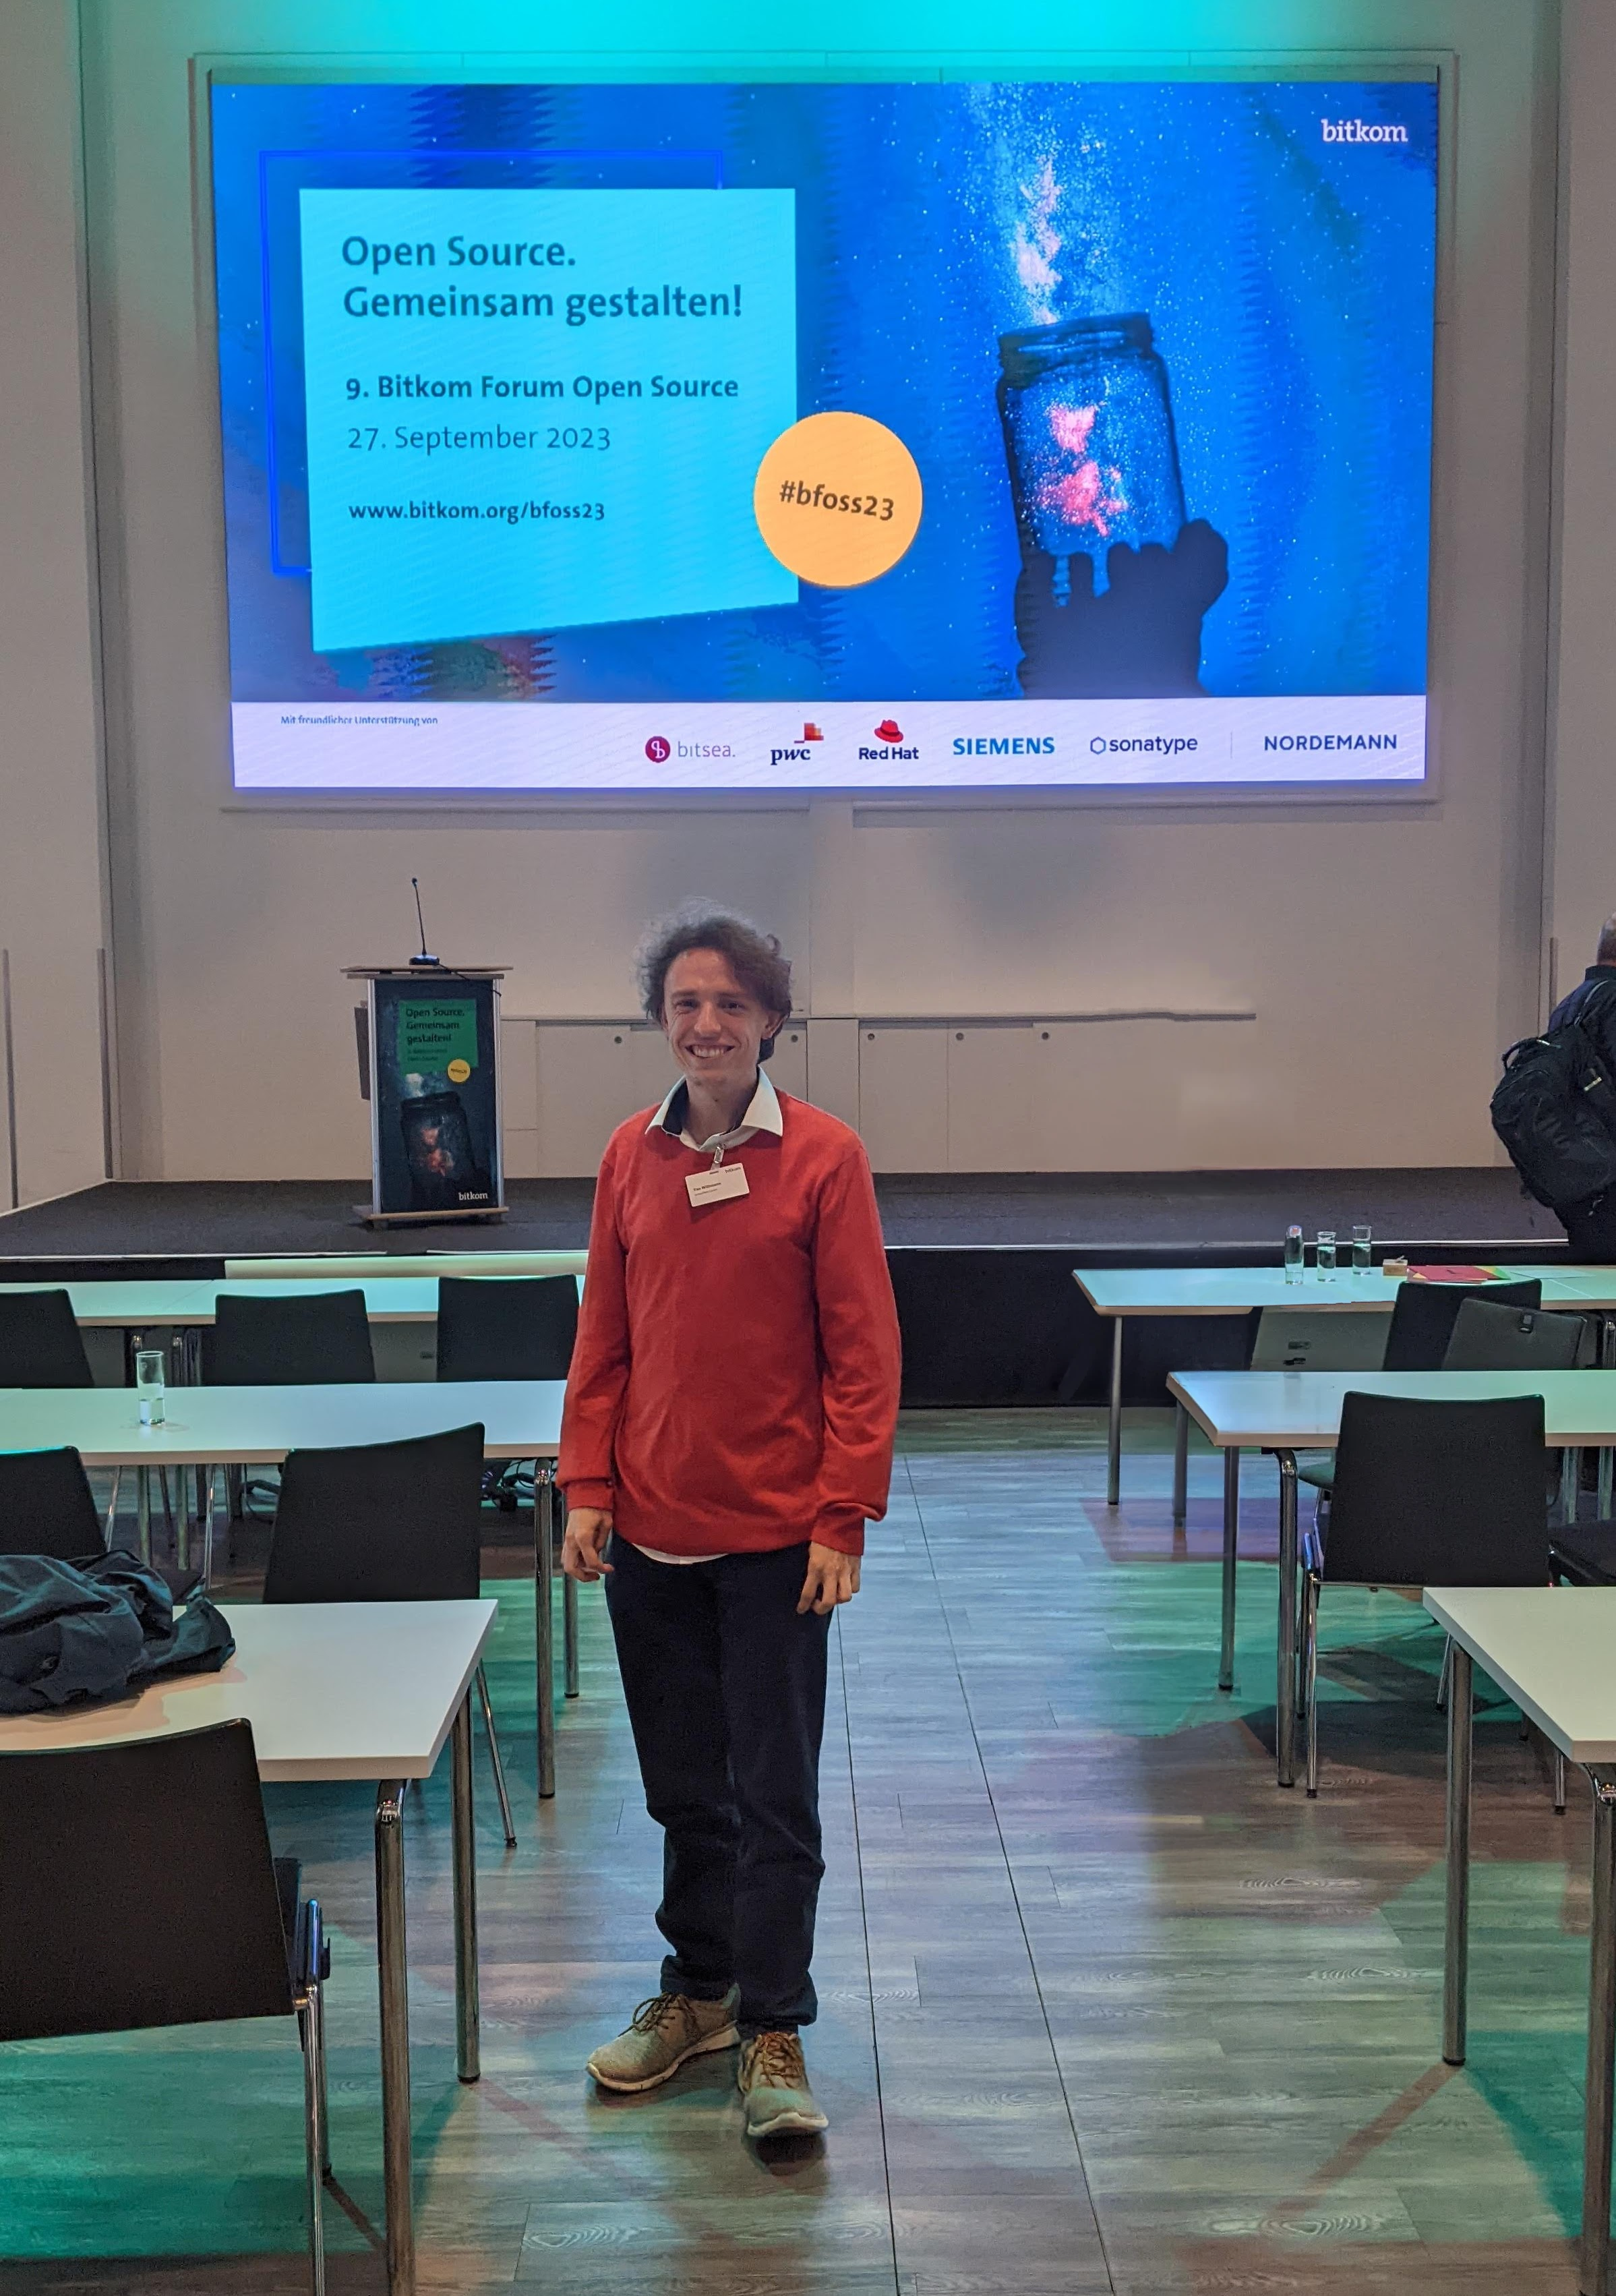
\includegraphics[width=0.5\textwidth, keepaspectratio]{res/img/2023-10-19-yan-ak-os}
    \caption{Auf dem Forum Open Source der Bitkom 2023}
    \label{fig:foss23-yan}
\end{figure}

Ein großer Programmpunkt war auch der {\bitkom} OpenSource Monitor\footnote{\url{https://www.bitkom.org/opensourcemonitor2023}}, der durch {\metaeffekt} gesponsert wird, wie in Abbildung \ref{fig:foss23-sponsor-metaeffekt} zu sehen ist.
Damit durfte die {\metaeffekt} einen Beitrag über den Cyber Resilience Act\footnote{\url{https://digital-strategy.ec.europa.eu/en/policies/cyber-resilience-act}} verfassen, der in diesem abgedruckt wurde.
Auch einige unserer direkten Kunden waren vertreten, die ich noch nie in Person getroffen hatte, außerdem konnte ich mit Studenten und Angestellten verschiedener Unternehmen sprechen.

\begin{figure}[htbp] % here, top, bottom, separate page
    \centering
    \includegraphics[width=0.8\textwidth, keepaspectratio]{res/img/2023-10-19-ak-os-metaeffekt-sponsor}
    \caption{Die {\metaeffekt} ist links als Sponsor zum OpenSource Monitor aufgeführt}
    \label{fig:foss23-sponsor-metaeffekt}
\end{figure}

\sweekdaymarginpar{\weekdayThursdayShort, \weekdayFridayShort}

Die Rückreise am Donnerstag verlief ohne Zwischenfälle, sodass der Freitag wieder der gewöhnliche Arbeitsalltag war.
Eine neue Kundenanforderung erforderte schon wieder direkte Aufmerksamkeit:
Einer unserer Download-Prozesse scheitert in ihrer Konfiguration, da der verwendete git-Befehl die konfigurierte Proxy-Informationen bislang scheinbar ignoriert.
Um das zu lösen, kann Git sowohl über einen Konfigurationsparameter im Befehlsaufruf, als auch über Umgebungsvariablen der Session konfiguriert werden.
Ich habe mich für die zweite Variante entschieden.

Ein persönliches Highlight war diesen Freitag allerdings, dass mein Bruder ab nächster Woche auch Teil des {\metaeffekt} Teams sein wird.


% Einarbeitung neuer Kollege (Nils)
\section{Woche 5 - Einarbeitung eines neuen Kollegen} \label{sec:bericht-wo-5}

% Woche 5 (2023-10-04 bis 2023-10-06)

\lweekdaymarginpar{\weekdayWednesdayLong}

Da Dienstag ein Feiertag war und ich montags einen Brückentag genommen hatte, war der Mittwoch mein erster Arbeitstag.
Die Einarbeitung meines neuen Kollegen war meine Hauptaufgabe für diese Woche.
Die Korrelationsdaten zu pflegen, also die Mappings zwischen unserer internen Darstellung von Software-Produkten und den Produkten in diversen externen Datenbanken, ist ab sofort sein Aufgabenbereich.
Passend dazu hat mein Chef uns einen neuen Datensatz gegeben, ein Inventar an Komponenten, den man einpflegen musste, anhand dem ich mit ihm die einfacheren Fälle und Grundlagen davon durchzugehen.

\sweekdaymarginpar{\weekdayThursdayLong}

Donnerstag habe ich erneut die etwas komplizierteren Fälle übernommen und ihn mit einigen einsteigerfreundlicheren versorgt.
Die Herausforderung für ihn als nicht-Informatiker an dieser Arbeit ist nicht nur die Methodik, sondern auch das gesammelte Wissen, das man über alle Software-Ökosysteme, Betriebssysteme und Software-Pakete haben muss.

\sweekdaymarginpar{\weekdayFridayLong}

Freitag habe ich ihm bereits etwas interessantere Fälle geben können und natürlich bei Fragen geholfen.
Ich bin etwas früher als er nach dem Weekly in das Wochenende gegangen.


% Weiter Daten-Korrelation & PowerShell Skripte
\section{Woche 6 - Daten-Korrelation \headerand PowerShell Skripte} \label{sec:bericht-wo-6}

% Woche 6 (2023-10-09 bis 2023-10-13)

\lweekdaymarginpar{\weekdayMondayShort\ - \weekdayWednesdayShort}

Da mein Kollege nicht das gesamte Inventar den Rest der Woche fertig bekommen würde, spielte sich diese Woche ähnlich wie letzte ab, in der ich meinen Kollegen bei der Arbeit unterstützte.
So konnte ich das Tool, das ich für diese Arbeit vor meinem Praktikum geschrieben hatte, selbst einmal anwenden und entdeckte einige Verbesserungsmöglichkeiten, die ich gleich umsetzte.
Das Tool (\qt{Correlation Utilities}) selbst ist Webapplikation, die mit einem lokal gehosteten Server, in Spring Boot implementiert, interagiert.
Das Ziel des Tools ist es, den Prozess des Mappings von unseren internen Produkten zu denen externer Datenbanken zu unterstützen.
Es aggregiert relevante Informationen automatisiert und macht Empfehlungen, wie am besten mit Fällen umgegangen werden sollte.
Dank des Tools besteht nun bereits fast keine Notwendigkeit, das ursprungs-Inventar zu durchsuchen oder Internet-Suchen zu starten.
Über die drei Tage habe ich es mit einigen weiteren Features erweitert.
Bis Mittwochabend hatten wir die Hälfte der Daten durchgearbeitet, den Rest sollte mein Kollege bis zum Ende der nächsten Woche erledigen.

\sweekdaymarginpar{\weekdayThursdayLong}

Donnerstag hatten mein Chef und ich morgens einen zweistündigen Termin mit einem unserer Kunden, {\aeclientZEZESE}, bei dem es um die automatisierte Erstellung einer SBOM (Software Bill of Materials) mit allen installierten Programmen, Treibern und Hardware-Devices auf Windows-Systemen ging.
Dieser Prozess sollte zweigeteilt sein:
Zunächst sollten über PowerShell-Skripte über Windows-Integrierte Features viele verschiedene Datenquellen angezapft und die rohen Ergebnisse in einem maschinenlesbaren Format in Dateien geschrieben werden.
Danach würde ein Maven-Plugin diese Daten analysieren und ein Inventar erzeugen.

Bis nächsten Montag sollten bereits erste Versionen der Skripte stehen.
Mein Arbeitslaptop selbst ist ein MacBook, also hat mir mein Chef einen zusätzlichen Windows-Laptop zum Entwickeln zur Verfügung gestellt.
An diesem habe mich zunächst einmal darüber informiert, wie man am besten an Windows-Systeminformationen gelangen kann.
Diese ersten Erkenntnisse habe ich zunächst in unserem internen Confluence niedergeschrieben, wo ich auch sonst meine Dokumentation ablege.

\sweekdaymarginpar{\weekdayFridayLong}

Freitag habe mich schnell wieder an das Thema gesetzt und mit den Ergebnissen meiner gestrigen Recherche angefangen, erste Skripte zur Sammelung von registrierten Programmen aus dem Store oder über Installers, die PNP-Devices (\qt{Plug and Play}) und Treibern.
Ich konnte die Hälfte der Use-Cases noch an diesem Tag durch verschiedene Skripte abdecken.


% PowerShell Skripte, Windows-Inventar & Strategieworkshop
\section{Woche 7 - Windows-Inventar-Extraktion \headerand Strategieworkshop} \label{sec:bericht-wo-7}

% Woche 7 (2023-10-16 bis 2023-10-20)

\lweekdaymarginpar{\weekdayMondayShort, \weekdayTuesdayShort}

Montag habe ich eine erste version der PowerShell Skripte fertigstellen können, die alle Use-Cases abdeckt.
Im Meeting später am Tag mit den Mitarbeitern von {\aeclientZEZESE} wurden meine Datensammlungs-Skripte dann live auf dem Ziel-Windows-Gerät erfolgreich ausgeführt.
Diese Daten auszuwerten hat gezeigt, dass sie noch nicht reichen, um ein vollständiges Bild zu erhalten, was ich dann den restlichen Tag durch Modifikationen an den Skripten geändert habe.

\sweekdaymarginpar{\weekdayWednesdayShort, \weekdayThursdayShort}

Die Entwicklung eines Java-Prozesses zur Verarbeitung von JSON-Daten aus PowerShell-Befehlen für ein Inventar im Format von {\metaeffekt} machte es nötig, die Ergebnisse der vielen verschiedenen PowerShell-Befehle zu kombinieren.
Wie bei Microsoft-Datenquellen so oft liefern die unterschiedlichen Befehle teils überlappende, teils einzigartige Datensätze, die nur zusammengenommen ein volles Bild ergeben.
Besonders bei Systeminformationen und PNP-Geräten waren Daten aus mehreren Befehlen zu konsolidieren.
Das Ergebnis war dann am Donnerstagabend ein vorläufiges Inventar, das zur Besprechung mit dem Kunden am Freitag noch etwas händisch aufbereitet wurde.

\sweekdaymarginpar{\weekdayFridayLong}

Der Freitag war ein ereignisreicher Tag:
Die {\metaeffekt} hat einen Strategieworkshop gehalten, der das Vorgehen der nächsten 9--12 Monate angeben sollte.
An einem großen Tisch und auf mehreren großen Whiteboard-Blättern wurden Wünsche und Pflichten aufgeschrieben und diskutiert.
Zu den Strategiepunkten, bei denen ich beteiligt sein werde, gehören die CVSS:4.0-Implementierung, eine Implementierung der CVSS-Versionen in TypeScript und eine Neuentwicklung des internen Datenmodells.

Das Meeting war sehr, hilfreich für mich, da es einen klaren roten Faden für das Semester vorgegeben hat.
Den Mitarbeitern von {\aeclientZEZESE} haben wir im Anschluss die Ergebnisse der Windows-Scans gezeigt und darum gebeten, dass sie die aktualisierten Skripte erneut ausführen, damit wir die vollständigeren Daten zu einem besseren Inventar umwandeln können.


% Abschluss Windows-Extraktion & Beginn Überarbeitung des Datenformats
\section{Woche 8 - Abschluss Windows-Extraktion \headerand Beginn Überarbeitung des Datenformats} \label{sec:bericht-wo-8}

% Woche 8 (2023-10-23 bis 2023-10-27)

\lweekdaymarginpar{\weekdayMondayShort, \weekdayTuesdayShort}

Mit den neuen Daten vom Freitag konnte ich Montag die Erkennung von Treibern, PNP-Devices und optionalen Features und die Performance des umfangreicheren Dateisystem-Scans einiger Skripte verbessern.
Um Dienstag die Windows-Extraktion vorerst abzuschließen, habe ich den restlichen Tag noch die PowerShell-Skripte unter einer MIT-Lizenz auf GitHub veröffentlicht und ein Maven-Plugin für die Inventar-Extraktion in Java geschrieben.

\sweekdaymarginpar{\weekdayWednesdayShort, \weekdayThursdayShort}

Mittwoch konnte ich (endlich) mit der Neuimplementierung der Datenstruktur und Logik dahinter beginnen.
Die einzelnen Tasks, die damit einhergehen, würden mich also die nächsten Wochen beschäftigen.
Bevor ich tatsächlich etwas programmieren konnte, wollte ich meine geplanten Änderungen in unserem internen Wiki dokumentieren und planen:
Begonnen habe ich mit dem Einführen eines Systems, das eine Quelle und Version eines Vektors eindeutig angeben kann.
Details dazu können in Kapitel \ref{subsec:projektbericht-loesungsweg-cvss-source-management} gefunden werden.
Eine erste Implementierung dazu konnte ich bereits Donnerstag fertigstellen.

\sweekdaymarginpar{\weekdayFridayLong}

Freitag habe ich damit verbracht, einem Kollegen zu helfen, der Probleme mit einer Software-Bibliothek hatte, die wir seit geraumer Zeit einsetzen.
Das Problem ließ sich am Ende auf einen internen Cache der Bibliothek zurückführen, den wir den Betreuern der Bibliothek in einem Issue\footnote{\url{https://github.com/spdx/Spdx-Java-Library/issues/215}} mitteilten.
Dieses Issue wurde einige Tage später durch einen Pull Request (PR) von meinem Kollegen behoben.


% Überarbeitung des Datenformats
\section{Woche 9 - Überarbeitung des Datenformats} \label{sec:bericht-wo-9}

% Woche 9 (2023-10-30 bis 2023-11-03)

\lweekdaymarginpar{\weekdayMondayLong}

Diese Woche begann ich mit der Überarbeitung des Datenformats für Schwachstellen und Security Advisories.
Das bisherige Datenformat besteht im Wesentlichen aus einer \codendt{Map<List<Map<String, String>\!>\!>}, wobei die einzelnen Ebenen zwar tatsächliche Instanzen mit weiteren Attributen und Methoden sind, aber sich nicht um das domänenspezifische  Parsen der Werte kümmern.

Dies bedeutet, dass komplexe Attribute oft über mehrere Schlüssel in der innersten Map verteilt sind oder aus einem strukturierten JSON-Objekt als String abgelegt werden.
Ein Problem dabei ist, dass man das Format dieser einzelnen Schlüssel genau kennen und es bei jedem Lese- und Schreibzugriff korrekt implementieren muss.

Obwohl Hilfsmethoden dafür zwar vorhanden sind, müssen diese trotzdem erst dem Entwickler bekannt sein und auch konsequent genutzt werden.
Es entsteht ein zusätzlicher Komplexitätsaufwand bei jeder Aufgabe, den man lieber vermeiden möchte.

Darum habe ich Montag ein System entworfen, das sich als Wrapper um die Zugriffe auf diese Klassen legt und dabei automatisch das korrekte (De-)Kodieren der Daten beim Ein- und Auslesen verwendet.

\sweekdaymarginpar{\weekdayTuesdayShort, \weekdayThursdayShort, \weekdayFridayShort}

Die Implementierung ist in zwei Schritten geplant, für jedes unserer betroffenen Module (core, artifact analysis).
Den Rest dieser Woche konzentrierte ich mich auf die Umsetzung des geplanten Systems in Artifact Analysis.
Dies beinhaltete vor allem die Entwicklung von Wrapper-Klassen für die inneren \code{Map<String, String>} Strukturen, die dafür verantwortlich sind, die Map in eine Kollektion von in unserem Datenmodell vorkommenden Instanzen umzuwandeln.
Zusätzlich plante ich eine Verwaltungsklasse, die für die korrekte Initialisierung aller Wrapper-Instanzen zuständig ist, diese verwaltet und die Verbindungsbeziehungen zwischen ihnen modelliert.

Die Programmierung dieser Komponenten erfolgte \qt{blind}, da ich den Code aufgrund von Konflikten zwischen dem bestehenden und dem neuen Datenmodell nicht ausführen konnte.
Das bestehende Datenmodell ist tief in unserer Codebasis integriert und stand an mehreren Stellen in Konflikt mit den neuen Strukturen.

Daher musste ich warten, bis die Änderungen in Artifact Analysis umgesetzt waren, was Freitagnachmittag \textit{fast} der Fall war.
Allerdings zog sich das wöchentliche Meeting länger als erwartet hin, wodurch ich die Umstellung diese Woche nicht vollständig abschließen und testen konnte.


% Abschluss Überarbeitung des Datenformats und CVSS Implementierung Verschieben
\section{Woche 10 - Abschluss Überarbeitung des Datenformats \headerand CVSS Implementierung Refactoring} \label{sec:bericht-wo-10}

% Woche 10 (2023-11-06 bis 2023-11-10)

\lweekdaymarginpar{\weekdayMondayLong}

Den Montag habe also damit verbracht, die Änderungen am Datenmodell und die Integration in die Prozessschritte in Artifact Analysis mit dem letzten verbleibenden Prozessschritt, dem VAD, zu vervollständigen\@.
Da hier alle Daten aggregiert dargestellt werden, ist dies einer der komplizierteren Schritte.
Zuerst ging es nur darum, die alte Funktionalität mit dem neuen Modell wiederherzustellen, ohne die neuen Features, die dadurch ermöglicht werden.
Einige Stunden später konnte ich immerhin den Code wieder ausführen, allerdings traten einige erwartete Fehler auf, die ich den restlichen Tag bearbeitete.

\sweekdaymarginpar{\weekdayTuesdayLong}

Die nächsten Tage konnte ich mich auf das Verschieben der CVSS-Implementierungen aus Artifact Analysis nach Core, in ein separates Modul, kümmern.
Die Aggregation der mehreren CVSS-Vektor-Quellen war zwar abgeschlossen, nun musste allerdings noch ein Prozess entworfen werden, der die Auswahl effektiver Vektoren und das korrekte Kombinieren und Überlagern ermöglicht.
Mit der Auswahl effektiver Vektoren habe ich den gesamten Dienstag verbracht, doch mein initialer Ansatz war zu naiv gedacht, weswegen ich die folgenden Tage einen neuen Ansatz verfolgte.

\sweekdaymarginpar{\weekdayWednesdayShort, \weekdayThursdayShort}

Mit diesem neuen Ansatz habe ich mir etwas länger Zeit gelassen, mit einigen Schaubildern und Testfällen zur Unterstützung.
Donnerstagnachmittag war der CVSS-Selektor dann fertig - deutlich komplizierter als anfangs erhofft, aber er konnte alle relevanten Fälle abdecken.

\sweekdaymarginpar{\weekdayFridayLong}

Um die Selektor-Logik in die bisherigen Prozessschritte einfügen war eine Nutzer-Konfiguration nötig, in der diese definierbar sind.
Ich habe in unserer Codebasis bereits ein recht umfangreiches Konfigurationssystem gebaut, was ich sehr einfach auf diesen Anwendungsfall anpassen konnte.
Mit meinem Chef zusammen habe ich beschlossen, dieses Konfigurationsobjekt auf alle Attribute auszuweiten, die etwas mit Security zu tun haben.
Diese neue zentrale Stelle habe ich vor und nach dem Weekly begonnen, überall zu integrieren und die alten Konfigurationsparameter durch diese auszutauschen.


% Transferieren der Datenklassen nach Core
\section{Woche 11 - Transferieren der Datenklassen nach Core} \label{sec:bericht-wo-11}

% 2023-11-13 bis 2023-11-17

\lweekdaymarginpar{\weekdayMondayLong}

Ende letzter Woche hatte ich die CVSS-bezogenen Features implementiert und in den Anreicherungsprozess integriert, sodass das System nun CVSS-Vektoren von beliebigen Datenquellen aufnehmen und deren Quellen nachvollziehbar halten konnte.
Den Montag nutzte ich, um diese Vektoren und deren berechneten Scores im VAD auf eine angereicherte Art anzuzeigen, was erstaunlich gut funktionierte.

\sweekdaymarginpar{\weekdayTuesdayLong}

Dienstagmorgen besprach ich mit meinem Chef die Integration dieser Änderungen in den PDF-Report unseres Core-Projekts.
Wir entschieden uns dazu, vorläufig Teile der Klassen in das andere Projekt zu kopieren, um auch dort Zugriff auf die Parsing-Logik zu haben, was zwar nicht schön ist (Code-Duplizierung), aber für jetzt die einfachere Lösung ist.
Noch am Dienstag konnte ich die relevanten Klassen in das Core-Projekt übernehmen und testen, wobei ich eine Namenskonvention für die kopierten Klassen festlegte und jeweils deren ursprüngliche Herkunft vermerkte.

\sweekdaymarginpar{\weekdayWednesdayShort, \weekdayThursdayShort, \weekdayFridayShort}

Mittwoch und Donnerstag stellte sich heraus, dass der Austausch des Datenmodells hinter dem PDF-Report mit dem kopierten Datenmodell komplexer war als erwartet.
Ich musste einige Abschnitte im Datenmodell leider komplett neu implementieren.
Den Rest der Zeit konnte ich dann das aktualisierte Modell in den Report einbinden.

Wir verwenden Apache Velocity mit einem textbasierten Template-XML-Format, was die Integration des neuen Modells aus mehreren Gründen sehr zeitintensiv machte.
Bis Freitagmittag war die Migration des Reports noch nicht abgeschlossen, allerdings hat war am Nachmittag ein Meeting mit einer Mitarbeiterin von \aeclientZEZESE\ geplant, um die Nutzung unseres VADs und die Bewertung von Schwachstellen in ihren Systemen zu besprechen.
Als Vorbereitung erstellte ich eine HTML-Seite, die unsere verschiedenen öffentlichen JSON-Schema-Dateien dynamisch zusammenfasst.
Das Meeting verlief erfreulicherweise angenehm und war produktiv für beide Seiten.


% Integration des Datenmodells in PDF-Report
\section{Woche 12 - Integration des Datenmodells in PDF-Report} \label{sec:bericht-wo-12}

% 2023-11-20 bis 2023-11-24

\lweekdaymarginpar{\weekdayMondayLong}

Am Montag erweiterte ich das Tracking-System der Matching-Konfigurationen aus verschiedenen Quellen von Schwachstellen, um nicht nur die bisherigen \qt{CPE}-Informationen, sondern auch Versionsbereiche und sogar Quellen wie GitHub und Microsoft zu integrieren.
Diese Informationen konnte ich noch am noch Montag in das VAD visuell ansprechend integrieren, was mir die Einfachheit von Anpassungen am VAD im Vergleich zum PDF-Report noch einmal deutlich machte.

\sweekdaymarginpar{\weekdayTuesdayShort, \weekdayWednesdayShort, \weekdayThursdayShort}

Die folgenden Tage kehrte ich wieder zur Integration des Datenmodells in den PDF-Report zurück.
Für jedes der etwa 20 Velocity-Templates ist der Prozess recht ähnlich:
Das Überprüfen der alten Datenzugriffe, im neuen Modell nach einem entsprechenden Zugriff suchen oder das Implementierte von neue Methoden, wiederholen sich stets.
Diese Änderungen nahm ich entweder in den Adapterklassen oder direkt im Modell vor, was Änderungen sowohl in Core als auch in Artifact Analysis erforderte.
Um den Dita-Renderingprozess (PDF-Generation aus Dita-Files) nicht bei jedem Test starten zu müssen, nutzte ich \qt{OxygenXML} für eine Live-Preview, doch der Prozess ist noch immer ein langer geblieben.

\sweekdaymarginpar{\weekdayFridayLong}

Freitag begann mit der Anfrage meines Chefs, ob ich an einem Workshop zum CSAF-Standard\footnote{\url{https://web.archive.org/web/20240121120954/https://www.allianz-fuer-cybersicherheit.de/Webs/ACS/DE/Netzwerk-Formate/Veranstaltungen-und-Austausch/CSAFversum/CSAFversum_node.html}} (Common Security Advisory Framework) teilnehmen möchte, der vom BSI in München organisiert wird.
Nach einer kurzen Recherche stimmte ich zu, da die Integration von CSAF in unser System schon länger geplant ist und mich persönlich auf eine Reise nach München freue.
Den Rest des Tages musste ich aufgrund der Abwesenheit eines anderen Kollegen erneut Korrelationsdaten für ein dringendes Inventar anlegen, bevor ich ins Wochenende starten konnte.


% Fertigstellung der Integration des Datenmodells & Dokumentation
\section{Woche 13 - Fertigstellung der Integration des Datenmodells \headerand Dokumentation} \label{sec:bericht-wo-13}

% 2023-11-27 bis 2023-12-01

\lweekdaymarginpar{\weekdayMondayShort, \weekdayTuesdayShort}

Nach einer Pause am Wochenende und der intensiven Report-Arbeit letzte Woche, konnte ich eben die Integration des Datenmodells in den Report bis Dienstagabend fast vollständig abschließen.
Dies schließt auch die neuen Segmente in den Templates zur Erklärung der Herkunft einer Schwachstelle ein.

\sweekdaymarginpar{\weekdayWednesdayShort, \weekdayThursdayShort}

Die Arbeit am neuen Datenmodell und Report war nun fast fertiggestellt.
Es blieben nur noch die Übersichtsdiagramme mit Statistiken über die gefundenen Schwachstellen für VAD (mit ChartJs\footnote{\url{https://www.chartjs.org}}) und PDF-Report (mit JFreeChart\footnote{\url{https://www.jfree.org/jfreechart}}) übrig.
Nachdem ich einige Zeit mit Reverse-Engineering der existierenden Diagramme verwendet hatte, musste ich zuerst einmal für zukünftige Zugriffe dokumentieren, welche Datenquellen wie verarbeitet werden und habe mit meinem Chef einige sinnvolle und lang geplante Änderungen an diesem Datenmodell besprochen.
Bis Donnerstag konnte ich das Thema des Refactorings des Datenmodells dann tatsächlich abschließen.

\sweekdaymarginpar{\weekdayFridayLong}

Da später im Praktikum diese Änderungen auch bei den Kunden angewendet werden müssen, habe ich am Freitag aus Voraussicht einen \qt{Migrationsguide} im internen Wiki erstellt, der alle Änderungen zwischen der alten und der neuen Generation unseres Systems dokumentiert.
Dieser Guide umfasst Themen wie die Änderungen an der CVSS-Implementierung, dem Tracking der CVSS-Vektoren und Schwachstellen, das neue Datenmodell, die neuen Konfigurationsparameter, neue Namenskonventionen und das restliche geändertes Verhalten.
Im Weekly Meeting berichtete ich, dass der neue Prozess nahezu abgeschlossen ist.


% Neuer Kollege, automatische Korrelationsdaten & Validierung des neuen Prozesses
\section{Woche 14 - Neuer Kollege, automatische Korrelationsdaten \headerand Validierung des neuen Prozesses} \label{sec:bericht-wo-14}

% 2023-12-04 bis 2023-12-08

\lweekdaymarginpar{\weekdayMondayLong}

Der Montag war auch der erste Arbeitstag eines neuen Kollegen, der uns bei der Entwicklung einer CI-Pipeline und eines Testing-Frameworks unterstützen sollte.
Ich half ihm vormittags bei der Einrichtung seines Laptops und erklärte ihm unsere Codebasis.
Nachmittags widmete ich mich einem anderen Kollegen, um über seine Änderungen an den Korrelationsdaten zu gehen, was den Rest des Tages in Anspruch nahm.

\sweekdaymarginpar{\weekdayTuesdayLong}

Diese gestrige Session mit den Korrelationsdaten erinnerte mich an die Art und Weise, wie wir Java-Versionen mit diesem System erkennen und, dass es nur ein provisorisches System sein sollte.
Ich entwarf Dienstag also ein System, das automatisch Korrelations-Einträge für alle bekannten Java-Versionen generieren kann.
Nach drei erfolglosen Iterationen über dieses Problem fand ich dann eine akzeptable und funktionierende Lösung und stellte sie dem Kollegen und meinem Chef vor.


\sweekdaymarginpar{\weekdayWednesdayShort, \weekdayThursdayShort}

In den folgenden Tagen nahm ich einen Schritt zurück, um den Refactoring-Prozess des Datenmodells noch einmal zu überprüfen.
Ich stellte fest, dass ich zwei größere Klassen vergessen hatte zu überführen und korrigierte zudem noch einige Fehler, die im Vergleich zu Generation 2 zu (zu stark) abweichenden Ergebnissen führten.
Nach diesen Korrekturen waren die Ergebnisse verbessert, und ich konnte endlich meine Generation 3 des Vulnerability-Monitorings meinem Chef präsentieren und besprechen.

\sweekdaymarginpar{\weekdayFridayLong}

Der bevorstehende CSAF-Workshop nächste Woche rückte näher, darum widmete ich den Freitag der Recherche über CSAF, indem ich die Dokumentation und einige Beispiele ansah.
Meine Erkenntnisse fasste ich in einem neuen Wiki-Artikel zusammen, wurde jedoch durch kleinere Anfragen und das wöchentliche Meeting immer wieder unterbrochen.
Die Recherche würde ich in der nächsten Woche fortsetzen.


% CSAF-Workshop in München
\section{Woche 15 - CSAF-Workshop beim BSI} \label{sec:bericht-wo-15}

% 2023-12-11 bis 2023-12-15

\lweekdaymarginpar{\weekdayMondayShort\ - \weekdayWednesdayShort}

Die Woche begann ich mit der Recherche zu CSAF, wobei ich mit der offiziellen Dokumentation\footnote{\url{https://docs.oasis-open.org/csaf/csaf/v2.0/os/csaf-v2.0-os.html}} begann.
Den Großteil der Zeit habe ich mich mit den JSON-Strukturen, Rollen der Teilnehmer, dem Produkt-Matching und den anderen Konzepten, die hinter CSAF stehen, beschäftigt.
Mir fielen einige Unterschiede zu anderen Standards auf, wie zum Beispiel, dass CSAF nicht nur das Format der Security Advisories definiert, sondern auch deren Veröffentlichung, Bereitstellung, Aktualisierung und Verarbeitung durch Endnutzer.
Diese Erkenntnisse hielt ich in einem Wiki-Eintrag fest und bereitete mich Mittwoch auf die Reise vor.

\sweekdaymarginpar{\weekdayThursdayLong}

Donnerstagmorgen reiste ich früh um 5:45 mit dem ICE zum Information Security Hub (ISH) des BSI am Flughafen München, wo der Workshop stattfand (Abbildung \ref{fig:yan-ish-csaf-muenchen}).

\begin{figure}[htbp] % here, top, bottom, separate page
    \centering
    \includegraphics[width=0.4\textwidth, keepaspectratio]{res/img/2023-12-14-yan-vor-dem-ish-muenchen}
    \caption{Vor dem \qt{Information Security Hub} am Münchner Flughafen}
    \label{fig:yan-ish-csaf-muenchen}
\end{figure}

Vor dem Workshop nutzte ich die Gelegenheit, mich mit anderen Teilnehmern von Bosch und anderen Unternehmen auszutauschen.
Der Workshop selbst war eine Mischung aus theoretischen Präsentationen und praktischen Übungen.
Es ging um die Begriffe, Rollen und Abläufe, aber auch um das tatsächliche Einsetzen der bereitgestellten Tools, dem eigenen erstellen von Security Advisories und dem Veröffentlichen dieser.
Besonders interessant waren für mich die Diskussionen über die Produktidentifikation und dem CVSS-Standard.
Nach dem Workshop und weiteren Gesprächen am abschließenden Buffet beendete ich den Tag mit einem Telefonat mit meinem Chef.

\sweekdaymarginpar{\weekdayFridayLong}

Freitag setzte ich die Teilnahme am Workshop fort, heute war der Fokus auf der praktischen Anwendung des CSAF-Standards.
Ich konnte, nachdem ich die Aufgaben recht schnell abschließen konnte, anderen Teilnehmern dabei helfen, die weniger Informatiker sind als Planer und Manager.
Nach dem Workshop und abschließenden Gesprächen machte ich mich auf den Heimweg und kam sogar dank einer früheren Verbindung schneller nach Hause.
Meine ausführlichen Notizen und Überlegungen würde ich in der folgenden Woche präsentieren.


% Letzte Woche vor der Weihnachtszeit
\section{Woche 16 - Letzte Woche vor der Weihnachtszeit} \label{sec:bericht-wo-16}

% 2023-12-18 bis 2023-12-20

\lweekdaymarginpar{\weekdayMondayLong}

Im Gegensatz zum letzten Jahr, wo das Weihnachtsfest ins Neujahr zurückverschoben werden musste, fand das Weihnachtsfrühstück der \metaeffekt dieses Mal frühzeitig im Schwarzen Walfisch statt.
Nach diesem gemeinsamen Frühstück kehrten wir ins Büro zurück, wo ich einen kurzen Bericht über den CSAF-Workshop für unsere Website verfasste\footnote{\url{https://metaeffekt.com/\#news}} und mit dem neuen Kollegen ein Testkonzept für unseren Software-Scanner diskutierte.

\sweekdaymarginpar{\weekdayTuesdayShort, \weekdayWednesdayShort}

Die restlichen Tage vor dem Urlaub widmete ich mich dem Abschluss des Refactorings meines Datenmodells, einschließlich Dokumentation und Code-Aufräumarbeiten.
Nach einem ausführlichen Gespräch mit meinem Chef über den Workshop konnte ich den Pull Request für die dritte Generation unseres Vulnerability Monitoring Toolings fertigstellen.
Mittwochabend ging ich gemeinsam mit den Kollegen in die Weihnachtsferien.


% TypeScript CVSS Calculator
\section{Woche 17 - TypeScript CVSS Calculator} \label{sec:bericht-wo-17}

% 2024-01-08 bis 2024-01-12

\lweekdaymarginpar{\weekdayMondayLong}

Das neue Jahr begann mit der Aufgabe, einen CVSS-Rechner in TypeScript zu entwickeln, der dann in ein zu entwickelndes Web-Interface integriert werden soll.
Dieses Interface soll die Scores für beliebig viele Vektoren, unabhängig von ihrer Version, berechnen und visualisieren können.
Für das gesamte Projekt ist später eine Veröffentlichung unter einer Open-Source-Lizenz auf GitHub vorgesehen.
Am Montag richtete ich zunächst das Projekt auf unserem lokalen git-Server ein, bereitete einen Build-Prozess mit Webpack vor und legte leere Klassen und Interfaces an.

\sweekdaymarginpar{\weekdayTuesdayShort\ - \weekdayFridayShort}

Die restliche Woche übersetzte ich die Java-Implementierungen in TypeScript und nutzte Jest\footnote{\url{https://jestjs.io/}} für Tests.
Ich erstellte einen Datensatz von 20.000 Vektoren pro CVSS-Version mit ihren erwarteten Scores für automatisierte Tests, anhand denen ich die Implementierungen entwickelte.
Bis zum Ende der Woche hatte ich die Klassen für CVSS:2.0 und CVSS:3.0 fertiggestellt und begann Freitag noch mit der komplexeren Version CVSS:4.0, konnte sie aber noch lange nicht fertigstellen.


% CVSS Calculator Web UI
\section{Woche 18 - CVSS Calculator Web UI} \label{sec:bericht-wo-18}

% 2024-01-15 bis 2024-01-19

\lweekdaymarginpar{\weekdayMondayShort, \weekdayTuesdayShort}

Den Beginn der Woche verbrache ich damit, die Implementierung von CVSS:4.0 abzuschließen.
Im Vergleich zur offiziellen JavaScript-Referenzimplementierung\footnote{\url{https://github.com/RedHatProductSecurity/cvss-v4-calculator/blob/main/app.js}} ist mein Ansatz in TypeScript deutlich objektorientierter und meiner Meinung nach übersichtlicher.
Zum Übernehmen der Implementierung einen eher ungewöhnlichen Ansatz gewählt, ich übertrug die Java-Klassen erst einmal 1:1 in TypeScript und passte sie dann Stück für Stück an die andere Sprache an.
Zirkuläre Referenzen löste ich mit madge\footnote{\url{https://www.npmjs.com/package/madge}}, aber ansonsten verlief alles in Ordnung.

\sweekdaymarginpar{\weekdayWednesdayShort, \weekdayThursdayShort, \weekdayFridayShort}

Nachdem alle Tests bestanden waren, implementierte ich das Web-Interface mit Bootstrap\footnote{\url{https://getbootstrap.com/}} und ChartJs.
Ich erstellte eine HTML-Struktur und entsprechendes JavaScript, um mit der CVSS-Bibliothek oder der NVD-API zu interagieren.
Nach der Basisfunktionalität verbesserte ich das UI, fügte Lizenzinformationen hinzu, räumte die Bibliothek auf und erstellte Dokumentation.
Das Ergebnis kann in Abb. \ref{fig:metaeffekt-cvss-calculator-ui} gesehen werden.
Das Projekt veröffentlichte ich auf GitHub\footnote{\url{https://github.com/org-metaeffekt/metaeffekt-universal-cvss-calculator}} und teilte es auf LinkedIn\footnote{\url{https://www.linkedin.com/feed/update/urn:li:activity:7151175714694729728/}}.
Das Feedback von unseren Kunden war sehr positiv, mit vielen Verbesserungsvorschlägen.

\begin{figure}[htbp] % here, top, bottom, separate page
    \centering
    \includegraphics[width=0.8\textwidth, keepaspectratio]{res/img/metaeffekt-cvss-calculator-ui}
    \caption{Der {\metaeffekt} Universal CVSS-Rechner}
    \label{fig:metaeffekt-cvss-calculator-ui}
\end{figure}

Von Herrn Shane Coughlan (OpenChain General Manager und ein Referent vom Open Source Forum der bitkom) haben wir freundlicherweise folgendes Zitat zu unserem Rechner erhalten:

\begin{quote}
    \textit{\qt{Contextualizing security threats is as important as identifying their existence,” says Shane Coughlan, OpenChain General Manager. “The emergence of open source tools to visualize this is a key part of ensuring the supply chain can plan ahead and action responses. We are delighted to see the work by Metaeffekt, an official OpenChain Partner, in the domain. It aligns well with OpenChain ISO/IEC 18974, the international standard for open source security assurance.}}
\end{quote}


%
\section{Woche 19 - Assessment-Policy \headerand Generation 3 Fertigstellung} \label{sec:bericht-wo-19}

% 2024-01-22 bis 2024-01-26

\lweekdaymarginpar{\weekdayMondayShort\ - \weekdayWednesdayShort}

Für einen unserer Kunden, der in die nächste Projektphase ihres Schwachstellmanagements gehen und nun Bewertungen vergeben möchte, erstellte ich den Anfang der Woche eine Assessment-Policy als Grundlage für ihre eigene Policy.
Das 6-seitige Dokument behandelt den Prozess des Vulnerability Monitorings, kontextualisiertes Re-Scoring mit CVSS, die Bedeutung einzelner CVSS-Metriken, die Vergabe von Status, Risiken und Maßnahmen sowie die Priorisierung von Schwachstellen.

\sweekdaymarginpar{\weekdayThursdayLong}

Zusammen mit einer Kollegin habe ich dieses Dokument Donnerstag noch einmal überarbeitet und an meinen Chef übergeben, der es auch noch einmal überarbeitet und dann mit unseren Kunden durchgesprochen hat.

\sweekdaymarginpar{\weekdayFridayLong}

Um die Änderungen der Generation 3 des Vulnerability Monitoring noch vor den Workshops des Kunden anzuwenden, wurde Freitag der große Pull Request endlich gemerged.
Den restlichen Tag habe ich weitere Anpassungen am CVSS-Rechner aufgrund von Feedback vorgenommen.
Es war zudem ein alter Kollege zu Besuch, mit dem wir nach der Arbeit noch einige Zeit verbrachten.


%
\section{Woche 20 - BSI-Meeting \headerand Integration von Generation 3} \label{sec:bericht-wo-20}

% 2024-01-29 bis 2024-02-02

\lweekdaymarginpar{\weekdayMondayLong}

Montags fand mit dem BSI ein Meeting bezüglich des CSAF-Standards und unseres CVSS-Rechners statt, mit Thomas Schmidt\footnote{\url{https://www.it-meets-industry.de/de/referent-thomas-schmidt}}, welcher bereits Leiter des CSAF-Workshops in München Ende letzten Jahres war, und Herr Von Samson.
Nach einer Demo unseres Toolings konnten wir nicht nur zur CSAF-Integration, sondern auch zum CVSS-Rechner, einige Tasks ableiten.
Thomas Schmidt erstellte in den folgenden Tagen dazu noch einige Issues auf unserem GitHub-Repository.

\sweekdaymarginpar{\weekdayTuesdayShort, \weekdayWednesdayShort, \weekdayThursdayShort}

Die restliche Woche startete dann die Integration von Generation 3 unseres Monitorings bei den mehreren Projekten unserer Kunden, um alle einheitlich von Generation 1 und 2 auf die neueste Generation 3 zu heben.
Der Prozess beinhaltete die Aktualisierung der Versionen und vor allem der Konfigurationen zum neuen Format, wobei der zuvor verfasste Migrationsguide wirklich sehr hilfreich war.
Trotz zahlreicher Komplikationen waren bis Donnerstagnachmittag alle Projekte aktualisiert.

\sweekdaymarginpar{\weekdayFridayLong}

Freitag bearbeitete ich die Issues\footnote{\url{https://github.com/org-metaeffekt/metaeffekt-universal-cvss-calculator/issues?q=is\%3Aissue+is\%3Aclosed}} von Thomas Schmidt, wobei bis auf Issue \#2 (keine Rückmeldung von FIRST\footnote{\url{https://www.first.org/cvss}} bis Praktikumsende) keine Probleme auftraten.
Nach unserem Weekly gab es ein Meeting mit einem Kunden zur finalen Integration der Generation 3 in ihre Pipeline.


%
\section{Woche 21 - Praktikumsbetreuung \headerand Abschluss des Praxissemesters} \label{sec:bericht-wo-21}

% 2024-02-05 bis 2024-02-09

\lweekdaymarginpar{\weekdayMondayLong}

Die letzte Woche meines Praktikums sollte ich einen BOGY-Praktikanten bei uns betreuen und die Integration von Generation 3 bei den Kunden fertigstellen.
Mit dem Praktikanten übte Montag ich Programmierkonzepte in Java, da er hauptsächlich Testfälle für unseren Software-Scanner und Komponenten-Extraktor schreiben sollte.

\sweekdaymarginpar{\weekdayTuesdayLong}

Der Praktikant konnte Konzepte schnell aufnehmen und begann Dienstag bereits mit den Testfällen.
Parallel dazu löste ich ein Problem mit der Laufzeit von Generation 3, das durch einen Programmierfehler von durchschnittlich 10 Minuten in Gen.\ 2 auf über zwei Stunden in Gen.\ 3 angestiegen war.
Eine kleine Code-Änderung (die Umwandlung einer Liste in ein Set) reduzierte die Laufzeit auf zweieinhalb Minuten, was uns natürlich alle beruhigte.

\sweekdaymarginpar{\weekdayWednesdayShort, \weekdayThursdayShort}

Mittwoch und Donnerstag behebte ich in einem Teams-Meeting in Live-Kooperation die letzten Probleme, sodass Generation 3 nun endlich überall vollständig integriert war.
Die restliche Zeit verbrachte ich mit dem Praktikanten und diversen Aufgaben.

\sweekdaymarginpar{\weekdayFridayLong}

An meinem letzten Tag brachte ich Kuchen mit und verteilte ihn beim Weekly.
Nach dem Meeting gingen wir gemeinsam Currywurst essen.
Ich behebte ein Issue mit einem unserer Reports, das durch die neue Filtermethode in Generation 3 entstanden war, und führte neue Parameter und alternative Report-Templates ein.
Der BOGY-Praktikant und ich beendeten mit dieser Woche unser Praktikum erfolgreich.
Ich arbeitete noch weitere 12 Tage bei dem Unternehmen und schloss einen Vertrag für weitere Zusammenarbeit ab.


    \else
    %! Author = Yan Wittmann


\chapter{Tätigkeitsbeschreibung} \label{ch:wochenberichte-initial}

Im Folgenden wird eine Beschreibung der Tätigkeiten über die Praktikumswochen gegeben.

% Einarbeitung in CVSS 4.0
\section{Woche 1 - Einarbeitung in CVSS 4.0} \label{sec:bericht-wo-1}

% Woche 1 (2023-09-4 bis 2023-09-8)

\lweekdaymarginpar{Montag}
Der erste Arbeitstag meines Praktikums bei der {\metaeffekt} fiel für mich mit dem Ende der Sommerpause für viele meiner Kollegen zusammen.
Da ich schon seit einiger Zeit im Unternehmen arbeite, war eine ausführliche Einführung für mich nicht nötig, denn ich habe bereits meine eigenen Aufgabenbereiche zugewiesen, um die ich mich kümmern muss.
Der Montag war allerdings auch für mich der erste Tag nach dem Urlaub, daher musste ich mich erst wieder orientieren und herausfinden, welche Aufgaben als Nächstes anstehen.

Ich verbrachte den Montag vor allem damit, einige Fehler zu korrigieren, die während der Urlaubszeit in unserem System in Kundenprojekten aufgetreten waren.
Ich führte auch Gespräche mit Kollegen, um zu klären, welche Projekte als Nächstes anstehen.
Ein wichtiges Thema war die anstehende Veröffentlichung des CVSS 4.0-Standards, die für den 31.\ Oktober 2023\footnote{\url{https://www.first.org/cvss/v4-0/}} geplant ist.
Es wurde entschieden, dass ich diesen Standard in den kommenden Tagen in unser System einpflegen sollte.
Unsere Software kann bereits die Score-Berechnungen für die CVSS-Versionen 2 und 3 durchführen, und wir möchten in der Lage sein, auch die neuen CVSS 4.0-Vektoren zu interpretieren und zu berechnen, sobald diese in den öffentlichen Datenbanken auftauchen.

Der eher ereignisreiche Montag endete damit, dass ich mit meinem Vorgesetzten und Betreuer für das Praktikum, Karsten Klein, vereinbart habe, während meines Vollzeitsemesters bei der {\metaeffekt} tägliche Meetings mit ihm abzuhalten.
Diese haben wir bisher jeden Tag durchgeführt und sowohl über berufliche als auch private Themen gesprochen.
Ich werde die genauen Inhalte dieser Meetings hier nicht immer aufführen, da sie meist über die bereits behandelten Themen des Tages gehen.

\sweekdaymarginpar{Dienstag}
Am Dienstag startete ich mit der Recherche zu den theoretischen Grundlagen und den Einzelheiten von CVSS 4.0.
Ich stellte schnell fest, dass es mehr Unterschiede als Gemeinsamkeiten zu den vorherigen Versionen CVSS 2 und 3 gibt, insbesondere in Bezug auf Berechnung, Implementierungsdetails, Interpretation der Ergebnisse und der Theorie dahinter.
Den Rest des Tages verbrachte ich damit, die noch unfertige Dokumentation und Beispiele des neuen Standards zu studieren und das Konzept zu verstehen, was sich als komplexer als zunächst angenommen erwies.

\sweekdaymarginpar{Mittwoch}
Am Mittwoch begann ich mit einem ersten Versuch einer Implementierung der CVSS 4.0-Berechnungen.
Nach weiterer Recherche fand ich auf dem offiziellen RedHat GitHub-Repository\footnote{\url{https://github.com/RedHatProductSecurity/cvss-v4-calculator}} den Quellcode einer Implementierung eines CVSS 4.0-Rechners in JavaScript.
RedHat war stark an der Entwicklung des Standards beteiligt.
Dieses Beispiel hat mir geholfen, das Grundgerüst für die Implementierung in unserem Java-System vorzubereiten, das dem Modell der CVSS 2 und 3 ähnelt.

\sweekdaymarginpar{Donnerstag}
Der Donnerstag startete mit einer Fehlermeldung in einem unserer Kundenprojekte.
Es handelte sich um eine „OutOfMemoryError“-Exception, die auftrat, wenn unser generierter Report zu Schwachstellen in Kundenprojekten aus einer bisher noch nicht so aufgetretenen großen Menge an Daten generiert werden sollte.
Das Problem war, dass während der Serialisierung in ein HTML-Dokument das interne Modell kurzzeitig dupliziert wurde und damit auch der Speicherbedarf.
Ich löste das Problem durch einen File Appender, der den HTML-String des Reports direkt in eine Datei schreibt, anstatt ihn wie zuvor im Speicher zu halten und habe so die kurzzeitige Verdoppelung den Hauptspeicher-Bedarf entfernt.

Der Hauptteil des Tages war jedoch weiterhin dem CVSS 4.0-Standard gewidmet.
Der Code der Referenz-Implementierung und die Spezifikation\footnote{\url{https://www.first.org/cvss/v4.0/specification-document}} haben mir erneut schwierigkeiten bereitet:
Nicht nur, dass der Code nicht sehr leserlich geschrieben war und viele verwirrende Muster verwendet, es gab auch einige Abweichungen zu der Spezifikation.
Ich meldete meine Probleme mit der Implementierung zusammen mit einigen inhaltlichen Fragen in einem Issue auf dem entsprechenden GitHub-Repository.
Ich beendete den Tag mit einer teilweise funktionierenden Implementierung.

\sweekdaymarginpar{Freitag}
Der Freitag sollte der Tag sein, an dem ich die Basis-Implementierung abschließe.
Es überraschte mich, dass ich so schnell auch eine Antwort auf meine GitHub-Fragen bekommen hatte: Die Spezifikation ist veraltet, aber die Implementierung ist korrekt.
Mithilfe dieser Informationen und einigem weiteren herumexperimentieren konnte ich die Berechnungen fertigstellen.
Ich validierte sie, indem ich einen großen Datensatz an zufälligen CVSS-Vektoren sowohl durch die Referenz-Implementierung und meine eigene laufen ließ und die Ergebnisse sich glichen.

Am Freitagmittag findet bei der {\metaeffekt} ein wöchentliches Meeting statt, das als \qt{Weekly} bezeichnet wird.
In diesem Meeting berichtet jedes Teammitglied über seine Fortschritte, Herausforderungen und nächsten Schritte.
Ich berichtete über meine Erfahrungen mit der Implementierung von CVSS 4.0 und hörte, was die anderen Teammitglieder in dieser Woche erreicht hatten.

Da ich am Freitagnachmittag private Verpflichtungen hatte, begann ich den Tag etwas früher und beendete meine erste Praktikumswoche nach dem „Weekly“-Meeting.


% Vertiefung in CVSS 4.0 und Korrelationsdaten
\section{Woche 2 - Vertiefung in CVSS 4.0 und Korrelationsdaten} \label{sec:bericht-wo-2}

\lweekdaymarginpar{Montag}
Die zweite Woche meines Praktikums wollte und sollte ich mich mit der genaueren Funktionsweise von CVSS 4.0 auseinandersetzen.
Ich verbrachte also den Montag damit, die Spezifikation\footnote{\url{htthttps://www.first.org/cvss/v4.0/specification-document}},
die Entwicklungsgeschichte\footnote{\url{https://www.first.org/cvss/v4.0/user-guide#New-Scoring-System-Development}}
und den Code tiefergehender anzusehen, um zu verstehen, wie die Berechnung des Scores funktioniert.

Ich hatte bereits während der Implementierung einen guten Überblick über den ersten Schritt der Berechnung, den mit den MacroVektoren, erhalten.
Die Unklarheiten lagen eher in dem zweiten Schritt: Der Interpolation zwischen den MacroVektor-Blasen.
Ich konnte selbst nach einem ganzen Tag an Recherche keine zufriedenstellende Erklärung finden, wie die Berechnung in diesem Schritt funktioniert.
Durch meine Recherche konnte ich immerhin weitere Randfall-Tests anlegen und damit zwei Fehler in meiner Implementierung finden.

\sweekdaymarginpar{Dienstag}
Eigentlich wollte ich am Dienstag weiter an meinem Verständnis von CVSS 4.0 arbeiten, aber es gab etwas Wichtigeres:
Da ein Kollege noch im Urlaub war, musste ich einen Teil seiner Arbeit übernehmen.
Es geht um das Pflegen von Korrelationsdaten, die dazu dienen, Software-Komponenten automatisch zu Produkten in fremden Datenbanken (wie den CPE in der NVD\footnote{\url{https://nvd.nist.gov/products/cpe}}) zuzuordnen.
Da dies früher einmal meine Aufgabe im Unternehmen war, habe ich dafür in der Vergangenheit ein Tool geschrieben, das ich kurz vor meinem Praktikum mit viel Feedback von und für meinen Mitarbeiter als Web-UI neu aufgesetzt hatte.
Das gab mir also die Chance, dieses Tool endlich einmal selbst zu verwenden und an einigen Stellen den Workflow zu verbessern.

\sweekdaymarginpar{Mittwoch}
Leider war ich Dienstag nicht mit den zu verarbeitenden Korrelationsdaten fertig geworden, darum habe ich noch den halben Mittwoch damit verbracht.
Was mich positiv überraschte war, wie gewissenhaft mein Kollege diese Arbeit durchgeführt hatte, seitdem er diese von mir übernommen hatte.
Ich musste nur bei wenigen Einträgen die Matching-Informationen überarbeiten, bei den meisten hatten diese bereits gestimmt und ich musste sie nur noch abnicken.

Den restlichen zwei Stunden habe ich dann noch mit meinem Chef über ein interessantes Thema reden können: Dem Abbilden von Vulnerability Chaining in unseren Systemen.
Also: was passiert, wenn man eine kritische Software-Schwachstelle, die man zuvor als \qt{Nicht Ausnutzbar} abgestempelt hatte, über eine andere, für sich alleine stehende harmlose, Schwachstelle ausnutzen kann?
Dieses Thema müssen wir auf Kundenwunsch in den nächsten Monaten abbilden können, aber eine hohe Priorität bekommt es noch nicht.

\sweekdaymarginpar{Donnerstag}
Donnerstag war mein Chef nicht im Büro, da er ein Treffen bei einem Kunden hatte.
Es war auch ein Tag, an dem ich sehr viel Code geschrieben habe, denn ich musste meine Planung für die Woche etwas umpriorisieren:
Ende der Woche musste die Implementierung und Integration von CVSS 4.0 in unser System fertiggestellt sein, darum beschloss ich, mich erst einmal darum zu kümmern und danach erst weiter mein Verständnis aufzubauen.
Die folgenden Punkte mussten bearbeitet werden:

\begin{smitemize}
    \item das Parsing der Vektoren aus verschiedenen Datenquellen/Formate (intern, extern)
    \item das korrekte Verarbeiten, wenn es um die Berechnung von Scores, das Modifizieren von Vektoren, oder das Ablegen in unseren Software-Inventaren geht
    \item das Anzeigen der Ergebnisse in unseren HTML- und PDF-Reports
\end{smitemize}

Da die externen Datenquellen ja noch keine Vektoren für CVSS 4.0 herausgeben, musste ich einige Annahmen über deren Formate machen, die ich bei tatsächlicher Veröffentlichung dann noch anpassen werde.

Bei diesen Arbeiten sind mir erst einige merkwürdige Muster in der Implementierung für die Berechnung der Scores aufgefallen, die ich mehr oder weniger aus der Referenz-Implementierung übernommen hatte.
Ich habe also fast noch einmal die gesamte Implementierung neu geschrieben, indem ich duplizierten Code in eigene Methoden und Klassen extrahiert und die Berechnungen wesentlich eleganter und näher an den dahinterliegenden mathematischen Modellen in meinem Programm abgebildet habe.

Am Ende des Tages hatte ich Pull Requests für die drei Projekte, in denen diese Berechnungen stattfinden, fertiggestellt.

\sweekdaymarginpar{Freitag}
Der Freitag begann frostig - im wahrsten Sinne des Wortes.
Es waren nur 7 °C und mit dem Fahrrad und kurzer Hose bin ich gut durchgefroren angekommen.
Mit einem Tee konnte ich mich aber ganz gut wieder aufwärmen.

Da ich die Integration bereits Donnerstag fertiggestellt hatte, habe ich mich wieder an das Verständnis über den CVSS 4.0 Standard gesetzt.
Um besser verstehen zu können, wie die MacroVektor Interpolation funktioniert, habe ich mir drei Beispiele herausgesucht und die Berechnungen aufgrund der Spezifikation und meiner Implementierung manuell mehrfach auf verschiedene Arten durchgeführt.
Das hat tatsächlich sehr geholfen und kurz vor dem Weekly hatte ich dann ein ganz gutes Verständnis, wie die Berechnung funktioniert.
Dies habe ich in einem Dokument für späteren Zugriff festgehalten.

Das Weekly war stark gefüllt, nicht nur ich hatte viele Neuigkeiten über die Funktionsweise von CVSS 4.0 zu berichten, sondern zwei meiner Kollegen hatten diese Woche auch in ihren Teilprojekten größere Durchbrüche, die sie sogar live demonstriert und erklärt haben.
Damit wurde das Weekly von einer Stunde auf fast zweieinhalb Stunden verlängert und der Tag war schnell herum.
Ich beendete meine zweite Woche mit einem guten Gefühl, diese Woche viel geschafft zu haben.


% Excel-Limitierungen & Präsentationsvorbereitung
\section{Woche 3 - Excel-Limitierungen \headerand Präsentationsvorbereitung} \label{sec:bericht-wo-3}

\lweekdaymarginpar{Montag}
Der Montag verlief eher ruhig, es gab keine größeren Themen, die dringend anstanden.
Darum lag mein Fokus daran, endlich einmal einige der Issues aus dem Jira-Backlog abzuarbeiten, die schon zu lange nötig waren.

Bei einem dieser Issues ging es darum, in unserem automatisierten CPE Matching-Algorithmus zwischen Hardware- und Software-Komponenten zu unterscheiden.
Dadurch würden wesentlich weniger false-positives entstehen, weil keine Softwarekomponenten mehr Hardware-CPEs zugeordnet werden würden.
Dazu war erst einmal eine Liste an Kategorien für Hardware nötig, die für die einzelnen Komponenten vergeben werden können.

Das Problem hierbei war der Detailgrad der Kategorien, welcher noch nicht festgelegt wurde.
Ich habe also nach einiger Recherche drei Vorschläge vorbereitet, die ich meinem Chef präsentierte.
Mein Chef und ich konnten uns recht schnell auf einen einigen, allerdings wollten wir uns noch eine Drittmeinung von einem Kollegen einholen.
Dieser hatte zu diesem Thema deutliche andere Meinungen, wie eine solche Liste auszusehen hatte.

Die Diskussion hierüber hat den gesamten restlichen Tag eingenommen und leider konnten wir bei keinem Ergebnis landen, mit dem alle zugestimmt hätten.
Wir machten aus, diese Diskussion an einem anderen Tag fortzuführen und damit war das Ende des Tages für mich erreicht.

\sweekdaymarginpar{Di, Mi, Do}

Die folgenden Tage konnte ich mich an etwas setzen, was ich schon lange in unserem Core-Projekt angehen wollte:
Es geht um die Serialisierung und Deserialisierung unserer Software-Inveterate zu Excel-Dateien.
Zellen speziell in Excel-Dokumenten haben ein Zeichenlimit von $32.767$\footnote{\url{https://support.microsoft.com/en-gb/office/excel-specifications-and-limits-1672b34d-7043-467e-8e27-269d656771c3}}, was in vielen unserer Fälle nicht ausreicht.
Seitdem ich bei der {\metaeffekt} bin, haben wir einen Workaround verwendet, der bereits in unserem Datenmodell nach einem System diese Zellen in mehrere Zellen aufteilt, sodass beim Serialisieren keine Probleme auftreten.
Das führt dazu, dass man nicht einfach so auf die betroffenen Felder in unserem Modell zugreifen kann, ohne speziell von dem Workaround Gebrauch zu machen.

Dass dies keine schöne Lösung ist, muss ich nicht erst sagen.
Probleme daran sind zum Beispiel:

\begin{smitemize}
    \item weiß jemand nicht von diesem Workaround, bekommt er vielleicht nur einen Bruchteil seiner Daten, wenn er die falsche Zugriffsart verwendet
    \item das Stylen der Excel-Zellen und Spalten funktioniert nicht richtig, da die Spalten aufgeteilt werden
    \item falls ein anderes Format mit niedrigerem Limit hinzugefügt werden soll, muss dieses Limit auch bei allen anderen Formaten so angewendet werden
\end{smitemize}

Ich war also recht froh, dass ich mich endlich einmal daran setzen konnte.
Ich habe die drei Tage nicht nur dazu genutzt, die Spaltung der Spalten in die Serialisierer zu verschieben, sondern auch ein allgemeines Styling-Modell einzuführen, das unabhängig vom Format auf Serialisierte Daten angewendet werden kann und einfach auf neue Formate angepasst werden kann.

\sweekdaymarginpar{Freitag}
Freitagmorgen wurde ich von meinem Chef erst einmal überrascht:
Nächste Woche Dienstag und Mittwoch sollte mit ihm und einer Kollegin nach Erfurt auf das Treffen des Arbeitskreises OpenSource\footnote{\url{https://www.bitkom.org/Bitkom/Organisation/Gremien/Open-Source.html}} unter dem Thema \qt{Open-Source-Communities} und das Forum OpenSource\footnote{\url{htthttps://www.bitkom.org/bfoss23}} der Bitkom gehe.

So weit, so gut.
Danach kam allerdings etwas, das ich nicht erwartet hätte: Ich sollte bei dem Treffen des Arbeitskreises OpenSource eine 25-Minütige Präsentation vor 30 Leuten von RedHat, Siemens, DB Systel und anderen großen Unternehmen über \qt{Identifikation und Bewertung von Schwachstellen mit Inhalten aus öffentlichen Quellen} halten.

Das kam überraschend, da ich noch nie auf einem solchen Treffen war und keine Ahnung hatte, wie eine solche Präsentation auszusehen hat.
Zum Glück hat mir mein Chef am Freitag noch geholfen, die wichtigen Themen aufzulisten und in eine sinnvolle Reihenfolge zu bringen.
Ich habe jedoch schnell gemerkt, dass die Zeit am Freitag und Montag nicht reichen werden, um die Präsentation vorzubereiten.
Ich habe zwar den Foliensatz an diesem Tag noch größtenteils fertigstellen können, aber das Skript hatte ich gerade erst angefangen zu verfassen.

\sweekdaymarginpar{Sa, So}
Und so kam das erste Mal, dass ich an einem Wochenende für die {\metaeffekt} gearbeitet habe.
Ich verbrachte das gesamte Wochenende damit, ein 11-seitiges Skript vorzubereiten, das alles enthält, was ich unbedingt in der Präsentation erwähnen wollte.
Natürlich habe ich die Präsentationsfolien weiter angepasst und mir Punkte notiert, die ich noch mit meinem Chef am Montag besprechen wollte.
Am Sonntagabend hatte ich dann ein Skript, mit dem ich zwar zufrieden war, aber irgendwie noch etwas fehlte.


% AK OpenSource & OpenSource Forum Erfurt
\section{Woche 4 - AK OpenSource \headerand OpenSource Forum Erfurt} \label{sec:bericht-wo-4-initial}

% Woche 4 (2023-09-25 bis 2023-09-29)

\lweekdaymarginpar{\weekdayMondayLong}

Nach einer kurzen Nacht, in der ich die letzten Feinschliffe an meinem Präsentationsskript anwendete, besprach ich Montag mit meinem Chef noch die letzten Unklarheiten.
Eines meiner Probleme bis jetzt war ein spezifischer Teil der Präsentation, der über ein Thema ging, mit dem sich zwar mein Chef gut auskennt, ich allerdings sehr wenig.
Mein Chef übernahm glücklicherweise kurzerhand diesen Teil.
Den Rest des Tages nutzte also ich lieber im Home-Office, um in Ruhe die Präsentation zu üben und meine Reisetasche für die morgige Reise nach Erfurt zu packen.

\sweekdaymarginpar{\weekdayTuesdayLong}

Der Dienstag begann früh mit unserer Reise mit dem ICE nach Erfurt.
Während der Zugfahrt nutzten mein Chef und ich die Zeit für eine letzte Durchsprache unserer Präsentation.
Angekommen in Erfurt ging es direkt in den nahegelegenen Räumlichkeiten der DB Systel.
Dort gab es zunächst einige einleitende Worte und eine Vorstandswahl, bevor ich mit meiner Präsentation dran war.

Meine Kollegen vor Ort haben mich noch einmal ermutigt und trotz anfänglicher Nervosität verlief alles reibungslos:
Ich war gut vorbereitet, hatte die Präsentation gut geübt und die Themen, die ich vorstellte, gehören zu meinem täglichen Arbeitsbereich seit drei Jahren.
Ich brauchte mein Skript kaum und das Feedback war ausschließlich positiv, was mich sehr gefreut hat, denn ich wollte wirklich einen Mehrwert in diese Runde bringen.

Abends wurde vom {\bitkom} eine Stadtführung und ein gemeinsames Abendessen mit anderen Teilnehmern des OpenSource Forums des nächsten Tages organisiert, an welchen wir teilnahmen.
Dort, und bereits beim Arbeitskreis, konnten wir uns auch mit den anderen Teilnehmern austauschen.

\sweekdaymarginpar{\weekdayWednesdayLong}

Das OpenSource Forum der {\bitkom} bot dann eine entspannte Alternative zum vorherigen Tag, bei dem die Teilnehmer vielfältige Präsentationen verfolgen und sich untereinander auszutauschen konnten.
Besonders spannend waren die Einblicke in die Open-Source-Strategien großer Unternehmen wie SAP, Siemens und Mercedes.
Die Parallelen im Bezug auf die aktuellen Herausforderungen und Lösungsansätze für die Verwaltung von Schwachstellen und Lizenzen von Open-Source-Software in ihren Produkten und Projekten haben mich etwas überrascht und bestätigten die Relevanz unserer Arbeit.

\begin{figure}[htbp] % here, top, bottom, separate page
    \centering
    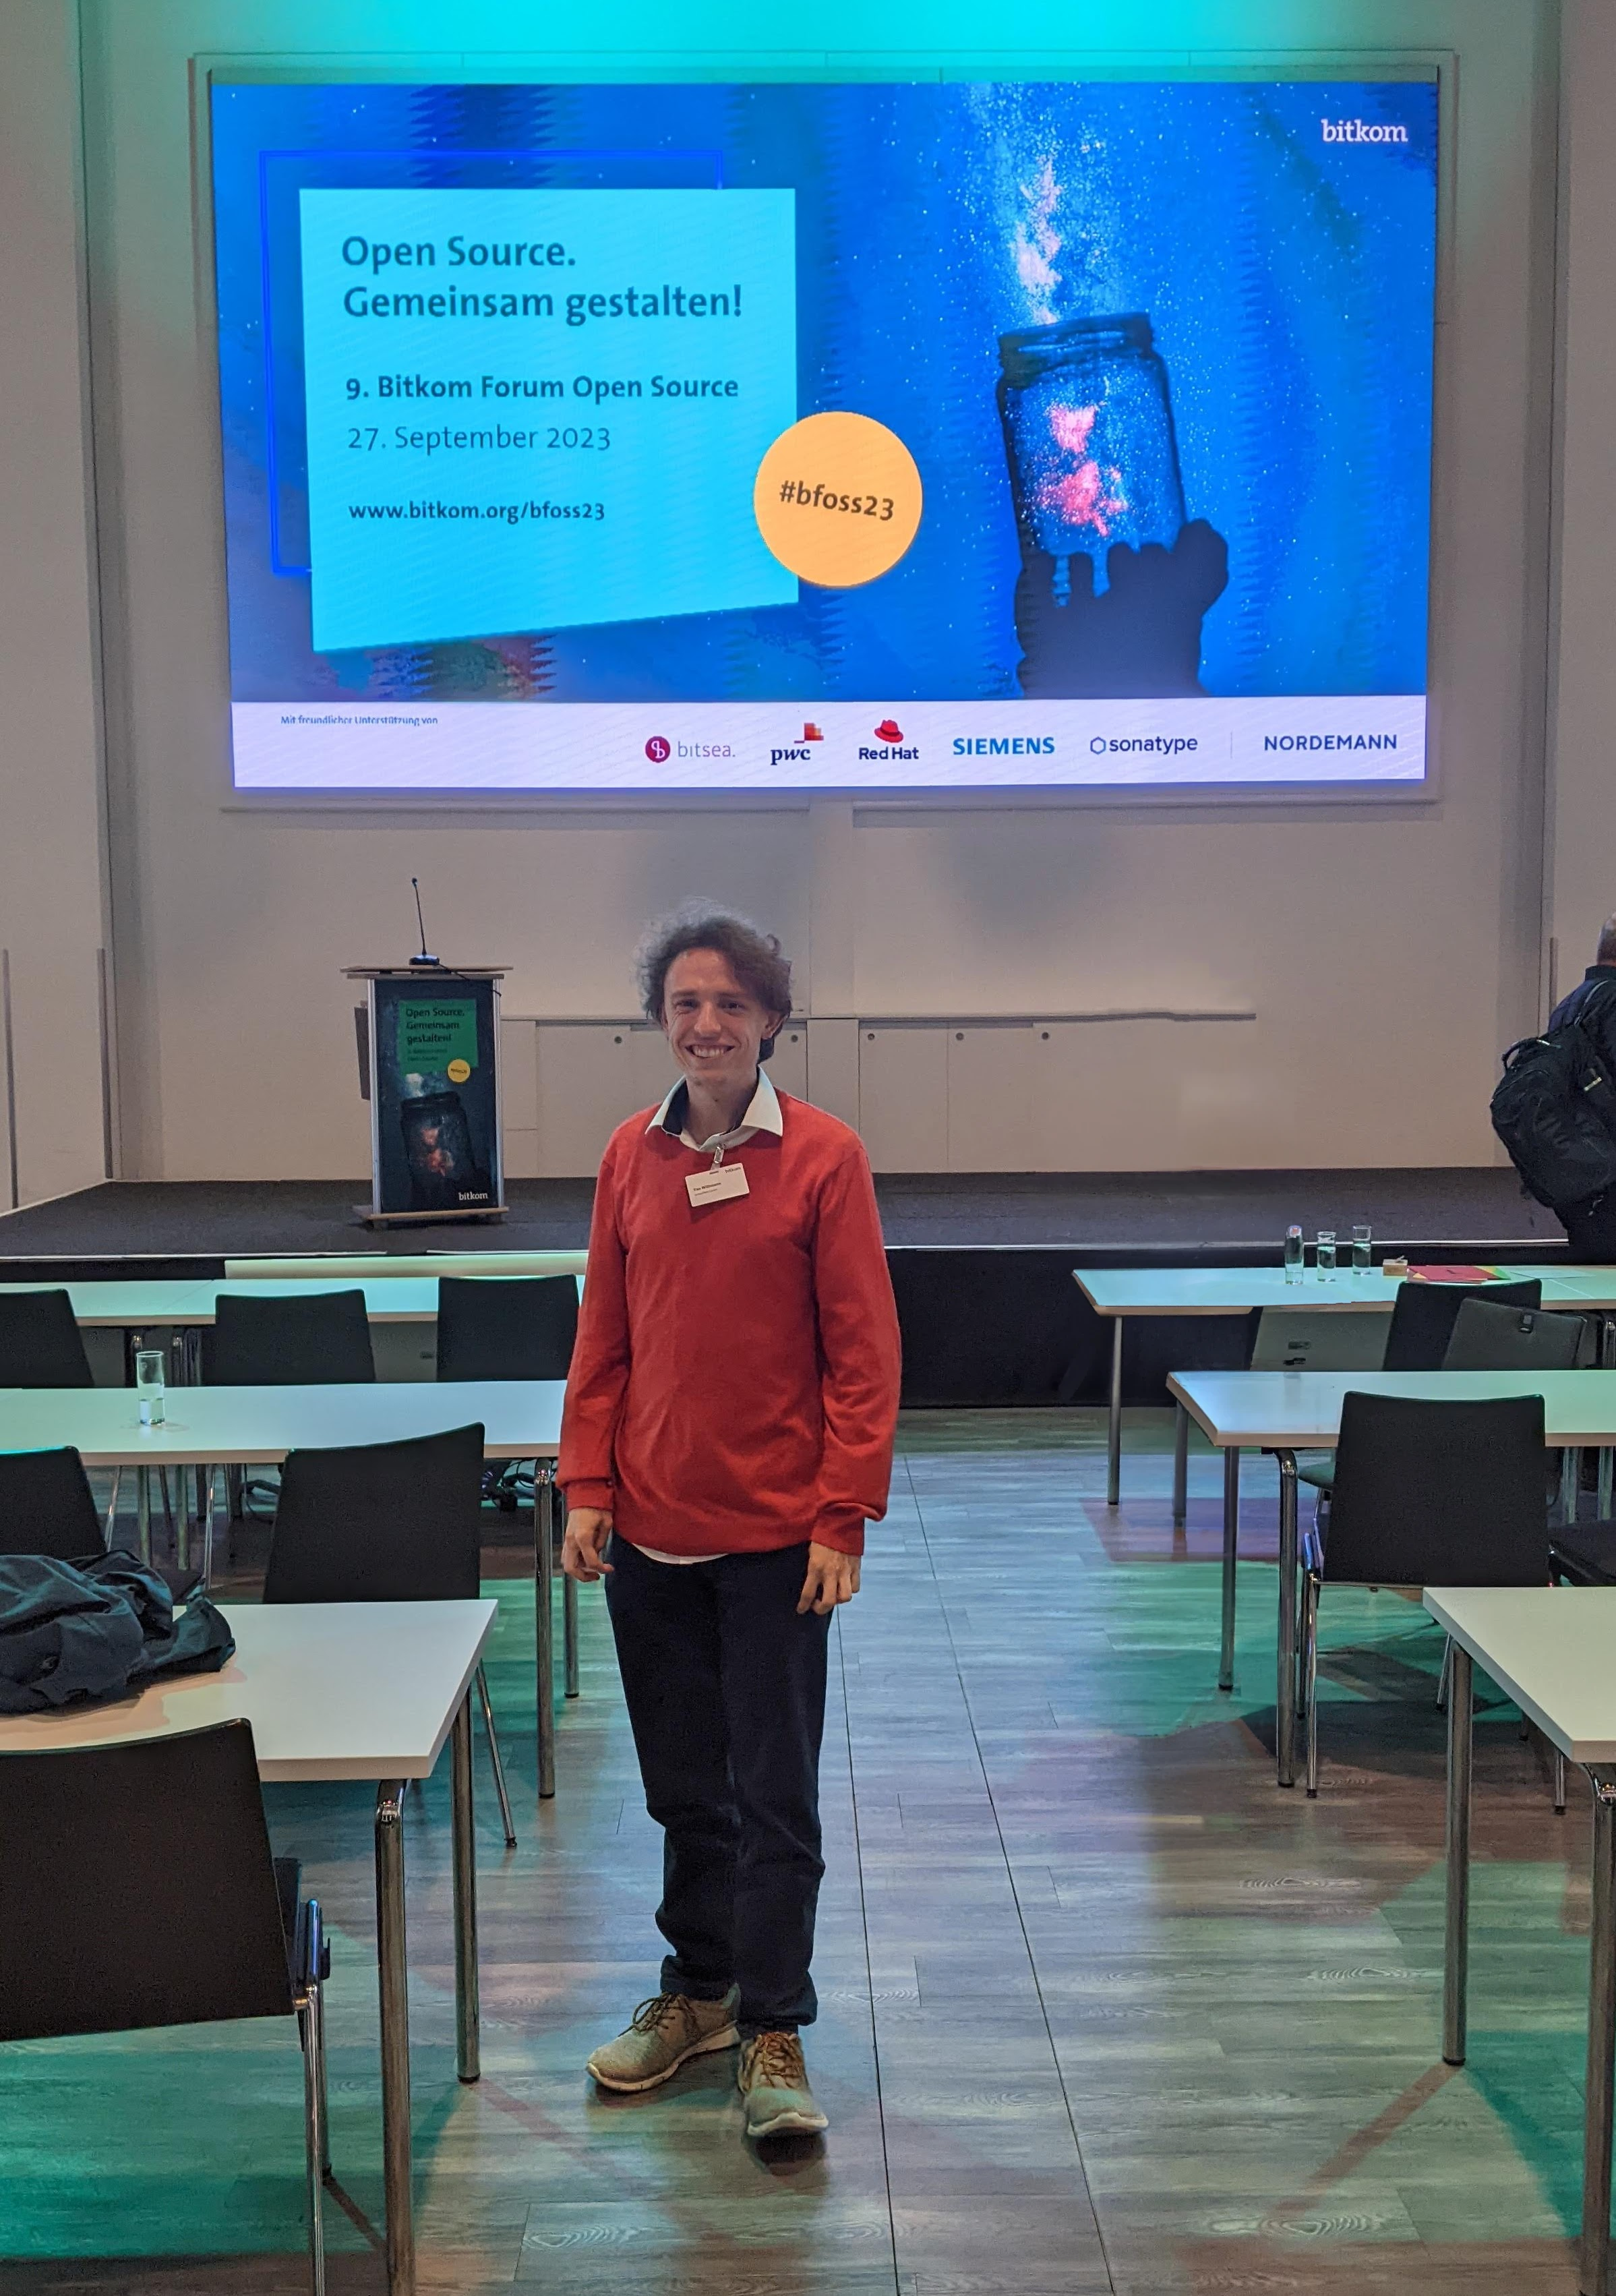
\includegraphics[width=0.5\textwidth, keepaspectratio]{res/img/2023-10-19-yan-ak-os}
    \caption{Auf dem Forum Open Source der Bitkom 2023}
    \label{fig:foss23-yan-initial}
\end{figure}

Ein großer Programmpunkt war auch der {\bitkom} OpenSource Monitor\footnote{\url{https://www.bitkom.org/opensourcemonitor2023}}, den die {\metaeffekt} gesponsert hat und damit einen Beitrag über den Cyber Resilience Act\footnote{\url{https://digital-strategy.ec.europa.eu/en/policies/cyber-resilience-act}} in diesem verfassen durfte.
Wir wurden auch auf der großen Leinwand aufgeführt, wie in Abbildung\ \ref{fig:foss23-sponsor-metaeffekt-initial} zu sehen ist.

\begin{figure}[htbp] % here, top, bottom, separate page
    \centering
    \includegraphics[width=0.8\textwidth, keepaspectratio]{res/img/2023-10-19-ak-os-metaeffekt-sponsor}
    \caption{Die {\metaeffekt} ist links als Sponsor zum OpenSource Monitor aufgeführt}
    \label{fig:foss23-sponsor-metaeffekt-initial}
\end{figure}

Es gab einige bekannte Gesichter vom vorherigen Tag, aber auch einige unserer direkten Kunden waren vertreten, die ich noch nie in Person getroffen hatte.
Außerdem hatte ich die fantastische Chance direkt mit Studenten und Angestellten verschiedener Unternehmen zu sprechen.

\sweekdaymarginpar{\weekdayThursdayShort, \weekdayFridayShort}

Die Rückreise am Donnerstag verlief ohne Zwischenfälle, sodass der Freitag wieder der gewöhnliche Arbeitsalltag war.
Eine neue Kundenanforderung erforderte schon wieder meine direkte Aufmerksamkeit:
Einer unserer Download-Prozesse scheitert in ihrer Konfiguration, da der verwendete git-Befehl die konfigurierte Proxy-Informationen bislang scheinbar ignoriert.
Um das zu lösen, kann Git sowohl über Umgebungsvariablen konfiguriert werden, als auch über einen Konfigurationsparameter im Befehlsaufruf.
Ich habe mich für die Umgebungsvariablen entschieden, die ich in der Prozess-Session, die über Java geöffnet wird, mit den Proxy-Informationen setzen kann.

Ein persönliches Highlight war diesen Freitag allerdings noch, dass mein Bruder nun auch Teil des Teams wird.
Über die letzten Tage hat er seine Bewerbung abgeschlossen, wurde angenommen und hat heute noch seinen Arbeitsvertrag unterzeichnet.
Er wird ab sofort die Korrelationsarbeiten des anderen Kollegen übernehmen.


% Einarbeitung neuer Kollege (Nils)
\section{Woche 5 - Einarbeitung eines neuen Kollegen} \label{sec:bericht-wo-5}

% Woche 5 (2023-10-04 bis 2023-10-06)

\lweekdaymarginpar{\weekdayWednesdayLong}

Da Dienstag ein Feiertag war und die {\metaeffekt} Montag einen Brückentag hatte, war der Mittwoch der erste Arbeitstag diese Woche und vor allem der erste für meinen neuen Kollegen.
Die Einarbeitung von ihm war meine Hauptaufgabe für diese Woche.
Sein Aufgabenbereich wird es sein, die Korrelationsdaten, also die Mappings zwischen unserer internen Darstellung von Software-Produkten und den Produkten in diversen externen Datenbanken, zu pflegen.
Passend dazu hat mein Chef uns einen neuen Datensatz gegeben, ein Inventar an Komponenten, den man einpflegen musste.
Diese Daten sollten bis zum Ende der nächsten Woche fertig sein.
Den Tag habe ich dann also dazu verwendet, mit ihm die Grundlagen unseres Systems und die Benutzung der von mir geschriebenen internen Tools, durchzugehen.

\sweekdaymarginpar{\weekdayThursdayLong}

Der Kollege hatte beschlossen, in seiner ersten Woche mehr als seine 10 Stunden zu arbeiten, darum konnte ich ihn am Donnerstag gleich wieder im Büro begrüßen.
Wir haben uns an die Software-Inventare gemacht, bei denen ich die etwas komplizierteren Fälle übernommen habe und ihn mit einigen einsteigerfreundlicheren versorgt habe.
Die Herausforderung an dieser Arbeit ist nicht nur die Methodik, sondern auch das gesammelte Wissen, das man über alle Software-Ökosysteme, Betriebssysteme und Software-Pakete haben muss, um die richtigen Entscheidungen treffen zu können.
Genau dieses Wissen ist, was ihm noch fehlt, dennoch hat er sich für einen ersten Tag sehr gut geschlagen.

\sweekdaymarginpar{\weekdayFridayLong}

Freitag startete ich mit den Inventaren zunächst ohne meinen Kollegen, der erst zum Weekly dazu kommen konnte.
Dieses Mal habe ich habe ihm etwas interessantere Fälle gegeben und natürlich bei Fragen geholfen.
Dies war das Ende der ersten Woche für ihn, der allerdings noch etwas länger dort verblieben ist, da er erst etwas später dazugekommen ist.


% Weiter Daten-Korrelation & PowerShell Skripte
\section{Woche 6 - Daten-Korrelation \headerand PowerShell Skripte} \label{sec:bericht-wo-6}

% Woche 6 (2023-10-09 bis 2023-10-13)

\lweekdaymarginpar{\weekdayMondayShort\ - \weekdayWednesdayShort}

Da mein Kollege nicht das gesamte Inventar den Rest der Woche fertig bekommen würde, spielte sich diese Woche ähnlich wie letzte ab, in der ich meinen Kollegen bei der Arbeit unterstützte.
So konnte ich das Tool, das ich für diese Arbeit vor meinem Praktikum geschrieben hatte, selbst einmal anwenden und entdeckte einige Verbesserungsmöglichkeiten, die ich gleich umsetzte.
Das Tool (\qt{Correlation Utilities}) selbst ist Webapplikation, die mit einem lokal gehosteten Server, in Spring Boot implementiert, interagiert.
Das Ziel des Tools ist es, den Prozess des Mappings von unseren internen Produkten zu denen externer Datenbanken zu unterstützen.
Es aggregiert relevante Informationen automatisiert und macht Empfehlungen, wie am besten mit Fällen umgegangen werden sollte.
Dank des Tools besteht nun bereits fast keine Notwendigkeit, das ursprungs-Inventar zu durchsuchen oder Internet-Suchen zu starten.
Über die drei Tage habe ich es mit einigen weiteren Features erweitert.
Bis Mittwochabend hatten wir die Hälfte der Daten durchgearbeitet, den Rest sollte mein Kollege bis zum Ende der nächsten Woche erledigen.

\sweekdaymarginpar{\weekdayThursdayLong}

Donnerstag hatten mein Chef und ich morgens einen zweistündigen Termin mit einem unserer Kunden, {\aeclientZEZESE}, bei dem es um die automatisierte Erstellung einer SBOM (Software Bill of Materials) mit allen installierten Programmen, Treibern und Hardware-Devices auf Windows-Systemen ging.
Dieser Prozess sollte zweigeteilt sein:
Zunächst sollten über PowerShell-Skripte über Windows-Integrierte Features viele verschiedene Datenquellen angezapft und die rohen Ergebnisse in einem maschinenlesbaren Format in Dateien geschrieben werden.
Danach würde ein Maven-Plugin diese Daten analysieren und ein Inventar erzeugen.

Bis nächsten Montag sollten bereits erste Versionen der Skripte stehen.
Mein Arbeitslaptop selbst ist ein MacBook, also hat mir mein Chef einen zusätzlichen Windows-Laptop zum Entwickeln zur Verfügung gestellt.
An diesem habe mich zunächst einmal darüber informiert, wie man am besten an Windows-Systeminformationen gelangen kann.
Diese ersten Erkenntnisse habe ich zunächst in unserem internen Confluence niedergeschrieben, wo ich auch sonst meine Dokumentation ablege.

\sweekdaymarginpar{\weekdayFridayLong}

Freitag habe mich schnell wieder an das Thema gesetzt und mit den Ergebnissen meiner gestrigen Recherche angefangen, erste Skripte zur Sammelung von registrierten Programmen aus dem Store oder über Installers, die PNP-Devices (\qt{Plug and Play}) und Treibern.
Ich konnte die Hälfte der Use-Cases noch an diesem Tag durch verschiedene Skripte abdecken.


% PowerShell Skripte, Windows-Inventar & Strategieworkshop
\section{Woche 7 - Windows-Inventar-Extraktion \headerand Strategieworkshop} \label{sec:bericht-wo-7}

% Woche 7 (2023-10-16 bis 2023-10-20)

\lweekdaymarginpar{\weekdayMondayShort, \weekdayTuesdayShort}

Montag habe ich eine erste version der PowerShell Skripte fertigstellen können, die alle Use-Cases abdeckt.
Im Meeting später am Tag mit den Mitarbeitern von {\aeclientZEZESE} wurden meine Datensammlungs-Skripte dann live auf dem Ziel-Windows-Gerät erfolgreich ausgeführt.
Diese Daten auszuwerten hat gezeigt, dass sie noch nicht reichen, um ein vollständiges Bild zu erhalten, was ich dann den restlichen Tag durch Modifikationen an den Skripten geändert habe.

\sweekdaymarginpar{\weekdayWednesdayShort, \weekdayThursdayShort}

Die Entwicklung eines Java-Prozesses zur Verarbeitung von JSON-Daten aus PowerShell-Befehlen für ein Inventar im Format von {\metaeffekt} machte es nötig, die Ergebnisse der vielen verschiedenen PowerShell-Befehle zu kombinieren.
Wie bei Microsoft-Datenquellen so oft liefern die unterschiedlichen Befehle teils überlappende, teils einzigartige Datensätze, die nur zusammengenommen ein volles Bild ergeben.
Besonders bei Systeminformationen und PNP-Geräten waren Daten aus mehreren Befehlen zu konsolidieren.
Das Ergebnis war dann am Donnerstagabend ein vorläufiges Inventar, das zur Besprechung mit dem Kunden am Freitag noch etwas händisch aufbereitet wurde.

\sweekdaymarginpar{\weekdayFridayLong}

Der Freitag war ein ereignisreicher Tag:
Die {\metaeffekt} hat einen Strategieworkshop gehalten, der das Vorgehen der nächsten 9--12 Monate angeben sollte.
An einem großen Tisch und auf mehreren großen Whiteboard-Blättern wurden Wünsche und Pflichten aufgeschrieben und diskutiert.
Zu den Strategiepunkten, bei denen ich beteiligt sein werde, gehören die CVSS:4.0-Implementierung, eine Implementierung der CVSS-Versionen in TypeScript und eine Neuentwicklung des internen Datenmodells.

Das Meeting war sehr, hilfreich für mich, da es einen klaren roten Faden für das Semester vorgegeben hat.
Den Mitarbeitern von {\aeclientZEZESE} haben wir im Anschluss die Ergebnisse der Windows-Scans gezeigt und darum gebeten, dass sie die aktualisierten Skripte erneut ausführen, damit wir die vollständigeren Daten zu einem besseren Inventar umwandeln können.


% Abschluss Windows-Extraktion & Beginn Überarbeitung des Datenformats
\section{Woche 8 -} \label{sec:bericht-wo-8}

% Woche 8 (2023-10-23 bis 2023-10-27)

\lweekdaymarginpar{Montag}



\sweekdaymarginpar{Dienstag}

\sweekdaymarginpar{Di, Mi, Do}


% Überarbeitung des Datenformats
\section{Woche 9 - Überarbeitung des Datenformats} \label{sec:bericht-wo-9}

% Woche 9 (2023-10-30 bis 2023-11-03)

\lweekdaymarginpar{\weekdayMondayLong}

Diese Woche begann ich mit der Überarbeitung des Datenformats für Schwachstellen und Security Advisories.
Das bisherige Datenformat besteht im Wesentlichen aus einer \codendt{Map<List<Map<String, String>\!>\!>}, wobei die einzelnen Ebenen zwar tatsächliche Instanzen mit weiteren Attributen und Methoden sind, aber sich nicht um das domänenspezifische  Parsen der Werte kümmern.

Dies bedeutet, dass komplexe Attribute oft über mehrere Schlüssel in der innersten Map verteilt sind oder aus einem strukturierten JSON-Objekt als String abgelegt werden.
Ein Problem dabei ist, dass man das Format dieser einzelnen Schlüssel genau kennen und es bei jedem Lese- und Schreibzugriff korrekt implementieren muss.

Obwohl Hilfsmethoden dafür zwar vorhanden sind, müssen diese trotzdem erst dem Entwickler bekannt sein und auch konsequent genutzt werden.
Es entsteht ein zusätzlicher Komplexitätsaufwand bei jeder Aufgabe, den man lieber vermeiden möchte.

Darum habe ich Montag ein System entworfen, das sich als Wrapper um die Zugriffe auf diese Klassen legt und dabei automatisch das korrekte (De-)Kodieren der Daten beim Ein- und Auslesen verwendet.

\sweekdaymarginpar{\weekdayTuesdayShort, \weekdayThursdayShort, \weekdayFridayShort}

Die Implementierung ist in zwei Schritten geplant, für jedes unserer betroffenen Module (core, artifact analysis).
Den Rest dieser Woche konzentrierte ich mich auf die Umsetzung des geplanten Systems in Artifact Analysis.
Dies beinhaltete vor allem die Entwicklung von Wrapper-Klassen für die inneren \code{Map<String, String>} Strukturen, die dafür verantwortlich sind, die Map in eine Kollektion von in unserem Datenmodell vorkommenden Instanzen umzuwandeln.
Zusätzlich plante ich eine Verwaltungsklasse, die für die korrekte Initialisierung aller Wrapper-Instanzen zuständig ist, diese verwaltet und die Verbindungsbeziehungen zwischen ihnen modelliert.

Die Programmierung dieser Komponenten erfolgte \qt{blind}, da ich den Code aufgrund von Konflikten zwischen dem bestehenden und dem neuen Datenmodell nicht ausführen konnte.
Das bestehende Datenmodell ist tief in unserer Codebasis integriert und stand an mehreren Stellen in Konflikt mit den neuen Strukturen.

Daher musste ich warten, bis die Änderungen in Artifact Analysis umgesetzt waren, was Freitagnachmittag \textit{fast} der Fall war.
Allerdings zog sich das wöchentliche Meeting länger als erwartet hin, wodurch ich die Umstellung diese Woche nicht vollständig abschließen und testen konnte.


% Abschluss Überarbeitung des Datenformats und CVSS Implementierung Verschieben
\section{Woche 10 - Abschluss Überarbeitung des Datenformats \headerand CVSS Implementierung Verschieben} \label{sec:bericht-wo-10}

% Woche 10 (2023-11-06 bis 2023-11-10)

\lweekdaymarginpar{Montag}

Den Montag habe also damit verbracht, die Änderungen am Datenmodell und die Integration in die Prozessschritte in Artifact Analysis zu vervollständigen.
Der einzige verbleibende Prozessschritt ist eine der Ausgaben des Systems: das VAD\@.
Dieses beinhaltet eine Aggregation aller Daten, die in den Schritten davor angereichert wurden und ist daher einer der komplizierteren Schritte.
Hierbei ging es mir nur darum, die alte Funktionalität wiederherzustellen, ohne die neuen Features, die durch das neue Datenmodell ermöglicht werden.
Ich muss hier dazusagen: Im Gegensatz zum alten Datenmodell war eine Freude, damit das UI zu befüllen, da die Daten einfach bereitliegen und ich sie nicht erst überall erneut und erneut berechnen muss.

Ein paar Stunden später konnte ich diesen Schritt abschließen und das Programm zu ersten Mal seit mehr als einer Woche ausführen.
Das Ergebnis war zu erwarten: natürlich hat die Hälfte der Schritte nicht funktioniert.
Ich habe den restlichen Tag noch alle (bis hier) auftretenden Probleme an dem Tag beheben können.

\sweekdaymarginpar{Dienstag}

Die nächsten Tage konnte ich mich auf das Verschieben der CVSS-Implementierungen aus Artifact Analysis nach Core, in ein separates Modul, kümmern.
Die Klassen zu verschieben habe ich innerhalb weniger Stunden erledigen können, bereits mit anpassung aller Imports und anderer Abhängigkeiten.

Eine der Anforderungen an das neue Datenmodell war, dass mehrere Vektoren gleicher Version mit unterschiedlichen Quellen auf der gleichen Schwachstelle abgelegt werden können.
An dieser hatte ich bereits mit den Quellen in Woche 8 (Kapitel\ \ref{sec:bericht-wo-8}) und bei dem neu-implementieren des Datenmodells gearbeitet.
Allerdings fehlten hier noch einige wichtige Komponenten, wie die Auswahl effektiver Vektoren und das korrekte Kombinieren und Überlagern von Vektoren.

Vor allem mit einer Datenstruktur für die Auswahl effektiver Vektoren habe ich den gesamten Dienstag verbracht.
Es stellte sich recht schnell heraus, dass mein initialer Ansatz zu naiv gedacht war und es schnell komplizierter wurde als erhofft.
Dienstag bin ich mit einem schlechten Gefühl nach Hause gegangen, denn der bisherige Ansatz hat nicht wirklich funktioniert.

\sweekdaymarginpar{Mi, Do}

Über den Feierabend hatte ich mir einige Gedanken zu dem Thema gemacht, wodurch ich durch die Erkenntnisse des vorherigen Tages am Mittwoch dann einen neuen Versuch an diesem System gewagt habe.
Mit diesem habe ich mir etwas länger Zeit gelassen, habe vernünftige Testfälle geschrieben und mir einige Schaubilder auf Papier gezeichnet.
Donnerstagnachmittag war der CVSS-Selektor dann fertig - deutlich komplizierter als ich anfangs erhofft hatte, aber nun konnte er alle Fälle abdecken, die mir und einem meiner Kollegen eingefallen sind.

\sweekdaymarginpar{Freitag}

Freitag wollte ich diesen Selektor in die bisherigen Prozessschritte einfügen, davor war allerdings etwas anderes nötig:
Eine Konfiguration, in der dieser vom Nutzer spezifiziert werden kann.
Ich habe in unserer Codebasis bereits ein recht umfangreiches Konfigurationssystem gebaut, was ich sehr einfach auf diesen Anwendungsfall anpassen konnte.

Nachdem ich mit meinem Chef noch einmal darüber geredet habe, haben wir beschlossen, dieses Konfigurationsobjekt für alle Attribute zu verwenden, die etwas mit Security zu tun haben, damit diese an einer zentralen Stelle abliegen und nicht in einzelnen Schritten versteckt sind.
Das habe ich getan, in der neuen \code{CentralSecurityConfiguration}.
Diese habe ich den Freitag, vor und nach dem Weekly, dann angefangen überall zu integrieren und die alten Konfigurationsparameter durch diese auszutauschen.


% Transferieren der Datenklassen nach Core
\section{Woche 11 - Transferieren der Datenklassen nach Core} \label{sec:bericht-wo-11-initial}

% 2023-11-13 bis 2023-11-17

\lweekdaymarginpar{\weekdayMondayLong}

Ende letzter Woche hatte ich also alle CVSS-bezogenen Features implementiert und in den Anreicherungsprozess integriert, sodass das System nun in der Lage war, CVSS-Vektoren von beliebigen Datenquellen aufzunehmen und deren Quellen nachvollziehbar zu halten.
Diesen Montag nutzte ich, um diese Vektoren und deren berechneten Scores im VAD, einem unserer Reporting-Outputs, anzuzeigen.
Um die effektiven Vektoren zu berechnen, musste ich auch die CVSS-Selektion anwenden, was erstaunlich gut funktionierte.

\sweekdaymarginpar{\weekdayTuesdayLong}

Dienstagmorgen besprach ich mit meinem Chef die Integration dieser Änderungen in den PDF-Report unseres Core-Projekts.
Wir konnten zwar zu dem Schluss kommen, dass es für die Codebasis sinnvoll wäre, sowohl das Datenmodell als auch das Reporting in separate Projekte auszulagern.
Wie so oft in der Informatik entschieden wir uns aufgrund von Zeitmangel jedoch für einen einfacheren Weg:
Wir kopierten Teile der Klassen in das andere Projekt, um auch dort Zugriff auf die Parsing-Logik zu haben.

Noch am Dienstag konnte ich die relevanten Klassen in das Core-Projekt übernehmen und testen.
Dafür legte ich eine Namenskonvention für die kopierten Klassen fest und vermerkte jeweils deren ursprüngliche Herkunft, um zukünftige synchronisationen zu vereinfachen.

\sweekdaymarginpar{\weekdayWednesdayShort, \weekdayThursdayShort}

Mittwoch und Donnerstag merkte ich, dass das Datenmodell hinter dem PDF-Report mit dem kopierten Datenmodell auszutauschen doch nicht so einfach ist, wie erhofft.
Ich musste darum einige Abschnitte im Datenmodell komplett neu implementieren.
Die größte Herausforderung war es allerdings, das aktualisierte Modell in den Report an sich einzubinden.
Wir verwenden Apache Velocity, um ein Template-XML-Format mit relevanten Daten zu füllen und Dita-Chapters zu generieren, die dann von einem Dita mit weiteren Style-Dokumenten zu einem PDF gerendert werden können.
Nicht nur, dass ich mich jedes Mal wieder neu in Velocity einarbeiten muss, wenn ich wieder am Report arbeite, sondern musste ich hier nun auch fast jede Zeile Logik in diesen Templates auf das neue Modell umstellen, was vor allem sehr Zeitintensiv war.

\sweekdaymarginpar{\weekdayFridayLong}

Bis Freitagmittag konnte ich die Migration des Reports zwar noch lange nicht abschließen, allerdings war am Nachmittag ein Meeting mit einer Mitarbeiterin von \aeclientZEZESE\ geplant.
Das Treffen zielte darauf ab, die Nutzung unseres VADs und die Bewertung von Schwachstellen mit Unterstützung unseres Systems zu besprechen.
Als Vorbereitung auf das Meeting erstellte ich eine HTML-Seite, die die verschiedenen öffentlichen JSON-Schema-Dateien unseres Prozesses dynamisch in verschiedenen Versionen zusammenfasst, Beispiele und Dokumentation anzeigt und Links zu den entsprechenden Versionen (oder \qt{latest}) generiert.

Das Meeting verlief sehr angenehm.
Wir kamen gut miteinander aus, und da sie hauptsächlich für das Verfassen von Dokumentationen und die interne Betreuung und das Verständnis unseres Prozesses bei ihnen verantwortlich ist, hat sie sich natürlich darüber gefreut, mit dem Hauptentwickler dieses Systems zu sprechen.


% Integration des Datenmodells in PDF-Report
\section{Woche 12 - Integration des Datenmodells in PDF-Report} \label{sec:bericht-wo-12}

% 2023-11-20 bis 2023-11-24

\lweekdaymarginpar{Montag}

Am Montag nahm ich mir eine kurze Auszeit von der Report-Migration und wendete mich einem anderen Aspekt des Refactorings zu:
Dem Tracking der genauen Matching-Konfigurationen von Schwachstellen, die aus verschiedenen Quellen identifiziert wurden.
Bisher beschränkt sich unser System auf das Tracking der \qt{CPE}-Informationen, allerdings ohne die dazugehörigen Versionsbereiche und auch nur bei diesen, nicht anderen Quellen.
In der Vergangenheit war das ausreichend, da nur die NVD als Datenquelle diente, aber mittlerweile kommen auch GitHub, Microsoft und andere hinzu.

Deshalb verbrachte ich den Tag damit, diese Daten in den verschiedenen Anreicherungsschritten in das von vor zwei Wochen implementierte Tracking-System einzupflegen.
Diese Informationen konnte ich noch am Montag in das VAD integrieren.
Bei dieser Gelegenheit wurde mir erneut bewusst, wie viel einfacher Anpassungen am VAD im Vergleich zum PDF-Report sind.

\sweekdaymarginpar{Di, Mi, Do}

In der Mitte der Woche konnte ich mich wieder vollständig auf die Integration des Modells in den Report konzentrieren.
Dieser Prozess ist stets gleich: Für jedes der etwa 20 Velocity-Templates in unserem Prozess überprüfe ich den alten Datenzugriff und suche ich im neuen Modell nach einem entsprechenden Zugriff oder implementiere neue Methoden.
Diese Änderungen mache ich entweder in den Adapterklassen, die als Schnittstelle zwischen Report und Modell dienen, oder direkt im Modell selbst.
In letzterem Fall muss ich die Änderungen sowohl in Core als auch in Artifact Analysis vornehmen.

Eine zusätzliche Herausforderung war, dass ich immer wieder auf Templates stieß, die ich zuvor noch nie gesehen habe und die ich erst verstehen musste.
Um nicht bei jedem Test den Dita-Renderingprozess starten zu müssen, nutze ich das Tool \qt{OxygenXML}, das eine Live-Preview ohne Stilelemente erlaubt.
Dennoch dauert es immer eine Weile, bis ich meinen Testdatensatz angepasst habe, um all diese Dokumente richtig testen zu können.

\sweekdaymarginpar{Freitag}

Freitag begann mit einer unerwarteten Anfrage meines Chefs:
Er fragte mich, ob ich Interesse hätte, alleine an einem Workshop zum CSAF-Standard\footnote{\url{https://web.archive.org/web/20240121120954/https://www.allianz-fuer-cybersicherheit.de/Webs/ACS/DE/Netzwerk-Formate/Veranstaltungen-und-Austausch/CSAFversum/CSAFversum_node.html}} (Common Security Advisory Framework) teilzunehmen, der vom Bundesamt für Sicherheit in der Informationstechnik (BSI) in München organisiert wird.
Nach einer kurzen Recherche zu CSAF fand ich heraus, dass es sich dabei um ein Schema handelt, ähnlich wie OSV\footnote{\url{https://osv.dev}}, das es Herstellern ermöglicht, Security Advisories und Informationen zu Schwachstellen in ihren Produkten zu veröffentlichen.

Der Hintergrund dieser Anfrage war, dass mein Chef plant, dass ich diesen Standard irgendwann in unser System integriere.
Da ich sowohl die Integration von CSAF als sinnvoll erachte, als auch persönlich mich auf eine Reise nach München freuen würde, stimmte ich dem Vorschlag zunächst einmal zu.

Den Rest des Freitags habe ich eine weitere Anfrage meines Chefs bearbeitet:
Das Anlegen von Korrelationsdaten für ein dringendes Inventar.
Dieser Prozess ist nicht besonders spannend, daher war ich froh, nach dem wöchentlichen Meeting ins Wochenende starten zu können.


% Fertigstellung der Integration des Datenmodells & Dokumentation
\section{Woche 13 - Fertigstellung der Integration des Datenmodells \headerand Dokumentation} \label{sec:bericht-wo-13}

% 2023-11-27 bis 2023-12-01

\lweekdaymarginpar{\weekdayMondayShort, \weekdayTuesdayShort}

Nach einer Pause am Wochenende und der intensiven Report-Arbeit letzte Woche, konnte ich eben die Integration des Datenmodells in den Report bis Dienstagabend fast vollständig abschließen.
Dies schließt auch die neuen Segmente in den Templates zur Erklärung der Herkunft einer Schwachstelle ein.

\sweekdaymarginpar{\weekdayWednesdayShort, \weekdayThursdayShort}

Die Arbeit am neuen Datenmodell und Report war nun fast fertiggestellt.
Es blieben nur noch die Übersichtsdiagramme mit Statistiken über die gefundenen Schwachstellen für VAD (mit ChartJs\footnote{\url{https://www.chartjs.org}}) und PDF-Report (mit JFreeChart\footnote{\url{https://www.jfree.org/jfreechart}}) übrig.
Nachdem ich einige Zeit mit Reverse-Engineering der existierenden Diagramme verwendet hatte, musste ich zuerst einmal für zukünftige Zugriffe dokumentieren, welche Datenquellen wie verarbeitet werden und habe mit meinem Chef einige sinnvolle und lang geplante Änderungen an diesem Datenmodell besprochen.
Bis Donnerstag konnte ich das Thema des Refactorings des Datenmodells dann tatsächlich abschließen.

\sweekdaymarginpar{\weekdayFridayLong}

Da später im Praktikum diese Änderungen auch bei den Kunden angewendet werden müssen, habe ich am Freitag aus Voraussicht einen \qt{Migrationsguide} im internen Wiki erstellt, der alle Änderungen zwischen der alten und der neuen Generation unseres Systems dokumentiert.
Dieser Guide umfasst Themen wie die Änderungen an der CVSS-Implementierung, dem Tracking der CVSS-Vektoren und Schwachstellen, das neue Datenmodell, die neuen Konfigurationsparameter, neue Namenskonventionen und das restliche geändertes Verhalten.
Im Weekly Meeting berichtete ich, dass der neue Prozess nahezu abgeschlossen ist.


% Neuer Kollege, automatische Korrelationsdaten & Validierung des neuen Prozesses
\section{Woche 14 - Neuer Kollege, automatische Korrelationsdaten \headerand Validierung des neuen Prozesses} \label{sec:bericht-wo-14-initial}

% 2023-12-04 bis 2023-12-08

\lweekdaymarginpar{\weekdayMondayLong}

Der Montag war auch der erste Arbeitstag eines neuen Kollegen, der uns in Teilzeit bei der Entwicklung einer CI-Pipeline und eines eigenen Testing-Frameworks für unsere Datenstrukturen unterstützen sollte.
Ich half ihm am Vormittag, unsere Projekte auf seinem Laptop einzurichten und verbrachte den halben Tag damit, ihm verschiedene Teile unserer Codebasis zu erklären.
Nach der Mittagspause übernahm mein Chef die Einarbeitung, und ich widmete mich einem anderen Kollegen, der Fragen zu einem Inventar und den von ihm erstellten Korrelationsdaten hatte.
Wir gingen gemeinsam über 40 Produkt-Mappings, um sicherzustellen, dass alles korrekt war.

Diese gestrige Überprüfung nahm zwar den Rest des Tages in Anspruch, war aber nützlich für meinen Kollegen:
Da er kein Informatiker ist, ist sein Wissen über die verschiedenen Ökosysteme und \qt{weit bekannte} Produkte begrenzt.
So konnte ich ihm verschiedene Paketmanager und Quellen für Paketinformationen zeigen.

\sweekdaymarginpar{\weekdayTuesdayLong}

Diese Session brachte mir ein länger bestehendes Problem in Erinnerung: die Art und Weise, wie wir Java-Versionen in diesem Datensatz erkennen.
Bisher hatte ich mich nicht getraut, Änderungen am Code davon zu machen, weil nicht alle Kunden die neueste Version nutzen und dieser Datensatz von allen verwendet wird.
Ich verbrachte den Dienstag damit, mit dem alten Code ein System zu entwerfen, das automatisch Einträge für alle bekannten Java-Versionen (etwa 2500 aus der NVD über CPE) generieren und den eingesetzten Java-Versionen unserer Kunden zuordnen kann.

Ich durchlief drei erfolglose Iterationen, die jeweils fast funktionierten, aber es fehlte immer ein entscheidendes Feature.
Die fehlenden Features waren ähnlich, aber unterschiedlich genug, sodass ich sie nicht direkt verwenden konnte.
Manchmal hatte ich das Gefühl, mein früheres Ich hätte diese Features absichtlich ausgelassen.
Zum Tagesende fand ich glücklicherweise eine funktionierende vierte Möglichkeit und legte dafür einen Testdatensatz an.

\sweekdaymarginpar{\weekdayWednesdayShort, \weekdayThursdayShort}

In den folgenden Tagen nahm ich einen Schritt zurück, um den Refactoring-Prozess des Datenmodells noch einmal zu überprüfen.
Abgesehen davon, dass ich vergessen hatte, zwei größere Klassen in das neue Modell zu überführen, wollte ich auch inhaltlich sicher sein.
In dem Security-Kontext unserer Applikation ist es besonders wichtig, dass die Ergebnisse entweder gleichbleiben oder sich verbessern, da Kunden korrekte Schwachstellen nicht übersehen sollen, nur weil sich unser Prozess verschlechtert hat.
Ich erstellte daher aus Bestandsdaten einige Testfälle und verglich die Ergebnisse mit der alten Version.
Einige der Ergebnisse unterschieden sich auf eine Weise, die nicht besser war als zuvor, welche sich dann allerdings recht Schnell auf konkrete Fehler in der Programmierung zurückführen ließen, die ich beheben konnte.

Donnerstagabend war für diesen Datensatz in jedem Fall die neue Version im Matching verbessert und Schwachstellen sind nur korrekt und nachvollziehbar verschwunden.
Diese Vergleichsdatensätze besprach ich auch noch einmal mit meinem Chef.

\sweekdaymarginpar{\weekdayFridayLong}

Der bevorstehende CSAF-Workshop nächste Woche rückte näher, darum widmete ich den Freitag der Recherche über CSAF, indem ich die Dokumentation und sah einige Beispiele ansah.
Meine bis dahin gesammelten Erkenntnisse fasste ich in einem neuen Wiki-Artikel zusammen.
Allerdings kam ich nicht so weit, wie ich gehofft hatte, da ich immer wieder durch kleinere Anfragen meines Chefs und das wöchentliche Meeting unterbrochen wurde.
Die Recherche würde ich dann in der nächsten Woche fortfahren.


% CSAF-Workshop in München
\section{Woche 15 - CSAF-Workshop beim BSI} \label{sec:bericht-wo-15-initial}

% 2023-12-11 bis 2023-12-15

\lweekdaymarginpar{\weekdayMondayShort\ - \weekdayWednesdayShort}

Wie geplant begann ich die Woche mit der Recherche zum Thema CSAF\@.
Die offizielle Dokumentation\footnote{\url{https://docs.oasis-open.org/csaf/csaf/v2.0/os/csaf-v2.0-os.html}} des Standards ist umfangreich, sodass ich den Großteil der Zeit damit verbrachte, die JSON-Strukturen und die Rollen der Teilnehmer zu verstehen.
CSAF definiert aber nicht nur das Format der Security Advisories, sondern auch deren Veröffentlichung, Bereitstellung, Aktualisierung und Verarbeitung durch Endnutzer.

Mir fiel auf, dass CSAF eine mir bisher noch nicht vorgekommene Methode zum Matchen von Produkten auf Advisories verwendet:
Zuerst muss pro Dokument ein Produktbaum verwendet werden, um durch die Knoten mit Bedingungen für die Nutzung der anliegenden Äste enthalten zu Blättern zu kommen, die jeweils ein Produkt identifizieren.
Diese Produkte werden dann in einer Sektion mit Kategorien wie \qt{affected} und \qt{not affected} aufgelistet, um herauszufinden, ob ein Produkt von einem Advisory betroffen ist.
Diese und weitere Erkenntnisse hielt ich in meinem Wiki-Eintrag fest und verließ Mittwoch das Büro etwas früher, um mich auf die Reise vorzubereiten.

\sweekdaymarginpar{\weekdayThursdayLong}

Am Donnerstagmorgen fuhr ich um 5:45 Uhr mit dem ICE nach München, wo ich glücklicherweise pünktlich ankam.
Von dort ging es mit der S-Bahn zum Münchner Flughafen, wo der zum Information Security Hub (ISH) des BSI liegt, dem Ort des Workshops.

\begin{figure}[htbp] % here, top, bottom, separate page
    \centering
    \includegraphics[width=0.5\textwidth, keepaspectratio]{res/img/2023-12-14-yan-vor-dem-ish-muenchen}
    \caption{Vor dem \qt{Information Security Hub} am Münchner Flughafen}
    \label{fig:yan-ish-csaf-muenchen-initial}
\end{figure}

Der vorherige Workshop war gerade zu Ende gegangen und die Teilnehmer, die auch am nächsten teilnehmen wollten, nutzten die 30-minütige Pause bis zum Beginn des nächsten, um sich auszutauschen.
Ich nutzte diese Gelegenheit, um einige Leute von Bosch und anderen Unternehmen kennenzulernen und mich mit ihnen über CSAF, über unser Unternehmen und andere Themen auszutauschen.

Der Workshop selbst bestand zur Hälfte aus einer theoretischen Präsentation, in der Begriffe, Rollen und Abläufe erklärt wurden, und zur anderen Hälfte aus praktischen Übungen an bereitgestellten Ubuntu-VMs.
Als Programmierer hatte ich keine Schwierigkeiten mit den Aufgaben und war oft der Einzige, der sie in der vorgegebenen Zeit abschließen konnte.
Das war vorteilhaft, denn so konnte ich noch mehr Menschen kennenlernen, indem ich auch ihnen bei den Aufgaben geholfen habe.

Besonders interessant waren allerdings die Diskussionen mit den Entwicklern des Standards.
Die Teilnehmenden hinterfragten einige Entscheidungen hinter CSAF und diskutierten, wie sich ihre individuellen Anwendungsfälle im Standard abbilden lassen.
Ich habe zu meinen eigenen Themen auch einige Fragen stellen können, wie unser Problem mit der uneindeutigen Produktidentifikation in verschiedenen Vendor- und Schwachstellendatenbanken und natürlich zum Thema CVSS, insbesondere zu den Herausforderungen mit vielen möglichen Vektoren für eine einzige Schwachstelle und zum neuen CVSS:4.0-Standard.

Nachdem der Workshop für den Tag beendet war und ich noch eine Weile am Buffet mit anderen Teilnehmern gesprochen hatte, ging ich zu meinem nahegelegenen Hotel.
Dort konnte ich den Tag nach einem kurzen Telefonat mit meinem Chef abschließen.

\sweekdaymarginpar{\weekdayFridayLong}

Freitagmorgen packte ich wieder früh um 5:30 im Hotel meine Sachen zusammen und checkte aus.
Zurück im ISH traf ich die Teilnehmer vom Vortag, konnte mich weiter austauschen und knüpfte weitere Kontakte.

Der Workshop begann mit einer weiteren Theorieeinheit zu den verschiedenen Rollen und Dokumentenarten, der Fokus lag aber heute auf der praktischen Anwendung des CSAF-Standards.
Unsere Aufgabe war es, die am Vortag eigens erstellten CSAF-Dokumente für die anderen Teilnehmer zugänglich zu machen, dann die der jeweils anderen herunterzuladen, zu validieren und zuletzt noch mit Python-Code zu verarbeiten.

Die Produktidentifikation war heute wieder ein großes Thema für die Teilnehmenden, da bisher vom Workshop nicht wirklich darauf eingegangen wurde, wie diese stattfinden sollte.
Für mich war das ebenfalls ein wichtiger Punkt, denn bei der \metaeffekt gibt es sogar eine Stelle, die sich nur mit der manuellen Zuordnung von Produkten aus Datenbanken zu unseren gescannten Komponenten befasst.
Eine richtige Lösung gibt es dafür scheinbar noch nicht, nur Ansätze, die so gut wie möglich in den Standard aufgenommen wurden.
Dies half zwar nicht wirklich unserem Problem weiter, es war aber auf jeden Fall gut zu hören, dass wir nicht die einzigen mit dieser Herausforderung sind.
In der dritten Version von CSAF möchten sie dieses Problem dann näher angehen.

Nach dem Ende des Workshops und abschließenden Gesprächen machte ich mich auf den Heimweg.
Dank einer Verspätung des ICE von Mannheim nach Heidelberg, wegen der die Zugbindung aufgehoben wurde, konnte ich eine frühere Verbindung nutzen und kam somit mehr als eine Stunde früher als geplant zu Hause an.
Die Erfahrungen teilte ich während der Fahrt mit meinem Chef, meine ausführlichen Notizen und Überlegungen würde ich dann in der folgenden Woche präsentieren.


% Letzte Woche vor der Weihnachtszeit
\section{Woche 16 - Letzte Woche vor der Weihnachtszeit} \label{sec:bericht-wo-16-initial}

% 2023-12-18 bis 2023-12-20

\lweekdaymarginpar{\weekdayMondayLong}

Im Gegensatz zum letzten Jahr, in dem das Weihnachtsfest der {\metaeffekt} ins neue Jahr verschoben wurde, schafften wir es dieses Mal, uns zum Weihnachtsfrühstück in einem Cafe in Heidelberg zu treffen.
Nach diesem Frühstück fuhren wir alle mit verschiedenen Verkehrsmitteln zurück ins Büro und arbeiteten den restlichen Tag.
Ich verfasste und veröffentlichte einen kurzen Paragrafen über den Workshop der letzten Woche für unsere Website\footnote{\url{https://metaeffekt.com/\#news}}.
Außerdem diskutierte ich mit dem neuen Kollegen über ein Testkonzept für die Ergebnisse unseres Software-Scanners.

\sweekdaymarginpar{\weekdayTuesdayShort, \weekdayWednesdayShort}

Die restlichen beiden Tage der Woche widmete ich mich nach der einwöchigen Pause wieder dem Refactoring meines Datenmodells.
Nachdem der Großteil der Features bereits implementiert war, konzentrierte ich mich nun auf Aufgaben wie die Dokumentation (extern und in JavaDoc), sowie allgemeine Aufräumarbeiten im Code.
Dienstag und Mittwoch verbrachte ich also damit, den Pull Request für die dritte Generation unseres Vulnerability Monitoring Toolings größtenteils fertigzustellen.
Ich nutzte auch die Gelegenheit, mit meinem Chef über den Workshop zu sprechen, was sich zu einem zweistündigen Gespräch entwickelte, da mehr zu besprechen und zu planen war als erwartet.

Diese Aufgaben konnte ich zufriedenstellend abschließen und ging dann am Mittwochabend gemeinsam mit den anderen in die Weihnachtsferien.


% TypeScript CVSS Calculator
\section{Woche 17 - TypeScript CVSS Calculator} \label{sec:bericht-wo-17-initial}

% 2024-01-08 bis 2024-01-12

\lweekdaymarginpar{\weekdayMondayLong}

Das neue Jahr begann nicht nur mit neuen Aufgaben, sondern auch mit einer neuen Programmiersprache: TypeScript.
Nach Abschluss des Datenmodell-Refactors konnte ich mich dem nächsten Projekt unserer Planung stellen, einem online-CVSS-Rechner.
Dieses Web-Interface soll in der Lage sein, für beliebig viele Vektoren, unabhängig von ihrer Version, die Scores zu berechnen und diese kompakt zu visualisieren.
Der erste Schritt bestand darin, die Versionen 2.0, 3.1 und 4.0 meiner Java-Implementierung in TypeScript zu übertragen.
Für das gesamte Projekt ist später eine Veröffentlichung unter einer Open-Source-Lizenz auf GitHub vorgesehen.
Den Montag lang habe ich das entsprechende Projekt erst einmal auf unserem lokalen git-Server eingerichtet, einen Build-Prozess mit Webpack vorbereitet und die leeren Klassen und Interfaces angelegt, die später befüllt werden sollen.

\sweekdaymarginpar{\weekdayTuesdayShort\ - \weekdayFridayShort}

Die restliche Woche verbrachte ich also damit, die Java-Implementierungen in TypeScript zu übersetzen.
Um sicherzustellen, dass meine Implementierung die Scores auch wirklich korrekt berechnet, nutzte ich Jest\footnote{\url{https://jestjs.io/}}, ein Testing-Framework für TypeScript-Projekte.
Dafür erzeugte ich durch den vorhandenen Java-Code einen Datensatz von 20.000 Vektoren pro CVSS-Version mit ihren erwarteten Scores, um die Tests automatisiert durchzuführen.

Da es die erste Woche des Jahres war und alle anderen erst noch ihre Prozesse und Aufgaben wiederaufnahmen, konnte ich mich ungestört auf dieses Projekt konzentrieren.
Bis zum Ende der Woche hatte ich daher die Klassen für CVSS:2.0 und CVSS:3.1 fertiggestellt und hatte bereits ein wenig mit der komplexeren Version CVSS:4.0 begonnen.
Allerdings fiel es mir am Freitagnachmittag nach einer ganzen Woche mit CVSS schwer, mich weiterhin zu konzentrieren, sodass ich froh war ins Wochenende zu gehen.


% CVSS Calculator Web UI
\section{Woche 18 - CVSS Calculator Web UI} \label{sec:bericht-wo-18}

% 2024-01-15 bis 2024-01-19

\lweekdaymarginpar{\weekdayMondayShort, \weekdayTuesdayShort}

Den Beginn der Woche verbrache ich damit, die Implementierung von CVSS:4.0 abzuschließen.
Im Vergleich zur offiziellen JavaScript-Referenzimplementierung\footnote{\url{https://github.com/RedHatProductSecurity/cvss-v4-calculator/blob/main/app.js}} ist mein Ansatz in TypeScript deutlich objektorientierter und meiner Meinung nach übersichtlicher.
Zum Übernehmen der Implementierung einen eher ungewöhnlichen Ansatz gewählt, ich übertrug die Java-Klassen erst einmal 1:1 in TypeScript und passte sie dann Stück für Stück an die andere Sprache an.
Zirkuläre Referenzen löste ich mit madge\footnote{\url{https://www.npmjs.com/package/madge}}, aber ansonsten verlief alles in Ordnung.

\sweekdaymarginpar{\weekdayWednesdayShort, \weekdayThursdayShort, \weekdayFridayShort}

Nachdem alle Tests bestanden waren, implementierte ich das Web-Interface mit Bootstrap\footnote{\url{https://getbootstrap.com/}} und ChartJs.
Ich erstellte eine HTML-Struktur und entsprechendes JavaScript, um mit der CVSS-Bibliothek oder der NVD-API zu interagieren.
Nach der Basisfunktionalität verbesserte ich das UI, fügte Lizenzinformationen hinzu, räumte die Bibliothek auf und erstellte Dokumentation.
Das Ergebnis kann in Abb. \ref{fig:metaeffekt-cvss-calculator-ui} gesehen werden.
Das Projekt veröffentlichte ich auf GitHub\footnote{\url{https://github.com/org-metaeffekt/metaeffekt-universal-cvss-calculator}} und teilte es auf LinkedIn\footnote{\url{https://www.linkedin.com/feed/update/urn:li:activity:7151175714694729728/}}.
Das Feedback von unseren Kunden war sehr positiv, mit vielen Verbesserungsvorschlägen.

\begin{figure}[htbp] % here, top, bottom, separate page
    \centering
    \includegraphics[width=0.8\textwidth, keepaspectratio]{res/img/metaeffekt-cvss-calculator-ui}
    \caption{Der {\metaeffekt} Universal CVSS-Rechner}
    \label{fig:metaeffekt-cvss-calculator-ui}
\end{figure}

Von Herrn Shane Coughlan (OpenChain General Manager und ein Referent vom Open Source Forum der bitkom) haben wir freundlicherweise folgendes Zitat zu unserem Rechner erhalten:

\begin{quote}
    \textit{\qt{Contextualizing security threats is as important as identifying their existence,” says Shane Coughlan, OpenChain General Manager. “The emergence of open source tools to visualize this is a key part of ensuring the supply chain can plan ahead and action responses. We are delighted to see the work by Metaeffekt, an official OpenChain Partner, in the domain. It aligns well with OpenChain ISO/IEC 18974, the international standard for open source security assurance.}}
\end{quote}


%
\section{Woche 19 - Assessment-Policy \headerand Generation 3 Fertigstellung} \label{sec:bericht-wo-19-initial}

% 2024-01-22 bis 2024-01-26

\lweekdaymarginpar{\weekdayMondayShort\ - \weekdayWednesdayShort}

Einer der Kunden der \metaeffekt, den wir mit dem Schwachstell-Monitoring betreuen, geht nun in eine Projektphase, in der er Einschätzungen für Schwachstellen und Maßnahmen für deren Mitigierung vergeben möchte.
Dazu planen sie interne Workshops verpflichtend für mehrere Abteilungen anzubieten, wobei wir sie natürlich unterstützen wollen.

Darum schrieb ich die erste Hälfte der Woche an einer Assessment-Policy als Ausgangspunkt für ihre Überlegungen.
In diesem 6 Seiten langen Dokument berühre ich die folgenden Punkte:
Was ist der allgemeine Prozess, Vulnerability Monitoring durchzuführen?
Wie kann mit CVSS ein kontextualisiertes re-Scoring stattfinden?
Was sind die einzelnen CVSS Metriken der verschiedenen Versionen, die (Kontext-weit) verändert werden können/sollten?
Wie vergibt man einen Status, Risiken und Maßnahmen?
Wie werden Schwachstellen am besten priorisiert?

\sweekdaymarginpar{\weekdayThursdayLong}

Zusammen mit einer Kollegin habe ich dieses Dokument Donnerstag noch einmal überarbeitet und an meinen Chef übergeben, der es auch noch einmal überarbeitet und dann mit unseren Kunden durchgesprochen hat.

\sweekdaymarginpar{\weekdayFridayLong}

Passend dazu war Freitag dann der Tag, an dem der große Pull Request mit der Generation 3 unseres Vulnerability Monitorings ge-merged wurde.
Uns ist es besonders wichtig gewesen, die Änderungen aus dieser Version noch vor den Workshops des Kunden anzuwenden, denn so müssen nicht gleich einen Monat später neue Kurse für die neue Version angeboten werden.
Diese Änderungen zum Kunden zu bringen würde aber erst nächste Woche geschehen.

Den restlichen Tag habe ich noch einige Änderungen aufgrund von Feedback, das wir erhalten haben, an unserem CVSS-Rechner gemacht.
Freitag war außerdem ein alter Kollege zu Besuch, der vor einiger Zeit aufgehört hatte, hier zu arbeiten.


%
\section{Woche 20 - BSI-Meeting \headerand Integration von Generation 3} \label{sec:bericht-wo-20-initial}

% 2024-01-29 bis 2024-02-02

\lweekdaymarginpar{\weekdayMondayLong}

Montag war ein interessanter Tag, denn heute hatten wir ein Meeting mit Repräsentanten vom BSI bezüglich des CSAF-Standards und unseres CVSS-Rechners.
Beteiligt war vor allem Thomas Schmidt\footnote{\url{https://www.it-meets-industry.de/de/referent-thomas-schmidt}}, welcher bereits Leiter des CSAF-Workshops in München Ende letzten Jahres war, und Herr Von Samson.

Hierfür habe ich den Morgen eine Demo unseres Toolings vorbereitet, welche wir dann am Nachmittag zusammen mit vorbereiteten Fragen durchgesprochen haben.
Insgesamt war es ein sehr konstruktives Meeting, aus dem wir viele weitere Tasks ableiten konnten, vor allem zu Ansätzen zur Integration von CSAF in unseren Workflow.
Thomas Schmidt hat die folgenden Tage noch einige Issues auf unserem Repository des CVSS-Rechners auf GitHub erstellt, die ich Ende der Woche angehen würde.

\sweekdaymarginpar{\weekdayTuesdayShort\ - \weekdayThursdayShort}

Die restliche Woche habe ich mich mit der Integration von Generation 3 unseres Monitorings bei den Kunden beschäftigt.
Einer unserer Problempunkte war es bisher, dass teilweise Kunden noch auf Generation 1 standen, diese wollten wir nun alle zusammen einheitlich auf Generation 3 heben.
Insgesamt mussten drei Projekte fürs Erste ge-upgraded werden.

Dafür habe ich von meinem Chef nacheinander Zugriff auf je einen Kundenlaptop bekommen, bei denen je ein- oder mehrere Git-Projekte mit unserem Tooling, welche in deren Pipelines verwendet werden.
Der Prozess war immer der gleiche:
die vorhandenen Versionen und Konfigurationen mussten alle der Reihe nach aktualisiert werden, sodass sie dem neuen Format entsprechen.
Hier war der Migrationsguide, den ich zuvor (für genau diese Situation) verfasst hatte, viel wert.

Es gab natürlich unzählige Komplikationen und genauso viele Änderungen, die noch am Code gemacht werden mussten, die hier aufgelistet den Rahmen sprengen würden.
Mittwochs bin ich auch etwas länger geblieben, aber Donnerstagnachmittag waren alle Projekte aktualisiert und liefen durch.

\sweekdaymarginpar{\weekdayFridayLong}

Freitag bin ich die Issues\footnote{\url{https://github.com/org-metaeffekt/metaeffekt-universal-cvss-calculator/issues?q=is\%3Aissue+is\%3Aclosed}} von Thomas durchgegangen und habe die ersten davon bearbeitet.
Hier gab es nichts, das Probleme bereitet hätte (bis auf Issue \#2, hier hat sich das FIRST\footnote{\url{https://www.first.org/cvss}} bis Praktikumsende nicht zurückgemeldet).

Zudem gab es nach unserem Weekly ein Meeting mit dem Kunden, der die Assessment-Workshops plant bezüglich der Generation 3, der Änderungen und es bei ihnen final in ihre Pipeline zu integrieren.


%
\section{Woche 21 - Praktikumsbetreuung \headerand Abschluss des Praxissemesters} \label{sec:bericht-wo-21-initial}

% 2024-02-05 bis 2024-02-09

\lweekdaymarginpar{\weekdayMondayLong}

Die letzte Woche für mich im Praktikum bedeutete den Start eines anderen:
Die {\metaeffekt} hat einen BOGY-Praktikanten angenommen, der diese Woche einmal bei uns reinschnuppern durfte.
Ich war zu einem großen Teil für seine Betreuung verantwortlich, nebenbei habe ich noch weitere Probleme mit der Integration von Generation 3 bei den Kunden gelöst, die seit dem Ende der letzten Woche aufgetreten sind.

Mit dem Praktikanten habe ich erst einmal ein wenig programmieren und Konzepte in Java geübt, denn er sollte diese Woche hauptsächlich mit einem der Testing-Frameworks eines anderen Kollegen einige Testfälle für unseren Software-Scanner und Komponenten-Extraktor schreiben.

\sweekdaymarginpar{\weekdayTuesdayLong}

Er schien Konzepte recht schnell aufzunehmen und so konnte er bereits Dienstag mit den eigentlichen Testfällen beginnen.
Natürlich hat er ab und zu auch andere Probleme lösen und Dinge tun dürfen.

Ansonsten ist der Dienstag genau wie der Montag verlaufen - ich durfte wieder Probleme mit Generation 3 beheben.
Allerdings schien dieses Mal ein größeres Problem dabei zu sein:
Unser Prozess ist auf einmal von durchschnittlich 10 Minuten Laufzeit auf Generation 2 zu über zwei Stunden auf der dritten gesprungen.
Das ist natürlich nicht akzeptabel, und ich habe mich gleich an die Recherche gemacht.
Gewundert hat es mich allerdings schon, denn ich hatte bei meinen Tests bei dem neuen Datenmodell speed-ups von bis zu 200\% oder 300\% in optimalen Fällen gemessen.

Glücklicherweise konnte ich das Problem mit nur einer Zeile Code-Änderungen beheben:
Ich habe eine Liste zu einem Set umgewandelt, eine Übersehene nicht vollständig durchgeführte Optimierung meinerseits, die ich scheinbar vergessen hatte, fertig durchzuführen.
Dadurch sind wir bei nur noch zweieinhalb Minuten gelandet, was eher dem entsprach, was ich erwartet hatte.

\sweekdaymarginpar{\weekdayWednesdayShort, \weekdayThursdayShort}

Mittwoch und Donnerstag habe ich noch live in Kooperation mit einem Teams-Meeting die letzten Probleme beheben können, passend zum Ende meines Praktikums war also Generation 3 vollständig integriert.
Natürlich konnte ich auch noch mit dem Praktikanten einige Dinge tun und üben.

\sweekdaymarginpar{\weekdayFridayLong}

An meinem 100sten und damit letzten Tag des Praktikums habe ich zur Feier Kuchen mitgebracht und beim Weekly zusammen mit den restlichen süßen Stückchen verteilt.
Nach dem Weekly konnten wir auch noch alle zusammen aus dem Büro Currywurst essen gehen, es war also ein guter Abschluss zum Praktikum.

Natürlich wurde auch gearbeitet:
Ich habe den Tag dazu genutzt, einem weiteren Issue meines Chefs mit einem unserer Reports zu beheben.
Hier ging es um den periodischen Security-Advisory Report mit Bezug auf die Schwachstellsituation in einem Projekt.
Durch die neue Art zu filtern in Generation 3 hat er bemerkt, dass er nun gerne genauer kontrollieren können möchte, welche Daten in diesem Report angezeigt werden.
Hier habe ich also neue Parameter und alternative Report-Templates angelegt, die diesen Wünschen entsprechen.

Auch für den BOGY-Praktikanten war es der letzte Tag und so sind wir beide mit einem erfolgreich absolvierten Praktikum ins Wochenende gegangen.

Ich habe noch weitere 12 Tage bei dem Unternehmen mit meinen 35 Stunden in den folgenden Wochen gearbeitet und einen weiteren Vertrag für weitere Zusammenarbeit abgeschlossen.
Meine Reise in dieser Welt ist also noch lange nicht vorbei.


    \fi

    %! Author = Yan Wittmann


\chapter{Projektbericht} \label{ch:projektbericht}

In der Einleitung (Kapitel\ \ref{sec:projektbericht-projektziel}) wird zunächst auf die Abteilung im Unternehmen, die aktuelle Situation und die Ziele für das Projektsemester eingegangen.
Bei den darauf folgenden Grundlagen (Kapitel\ \ref{sec:projektbericht-grundlagen}) werden die relevanten Themen, Begriffe und Standards erklärt.


\section{Einleitung, Problemstellungen und Projektziel} \label{sec:projektbericht-projektziel}

Die für dieses Praktikum relevante Abteilung in der {\metaeffekt} stellt ein automatisiertes Vulnerability Monitoring her und integriert es bei diversen Kunden, deren Wünsche und Anforderungen priorisiert in die Systeme zurückgeführt werden.
Das Vulnerability Monitoring wird intern durch eine Aneinanderreihung von Prozessschritten modelliert, die auch als \qt{Inventory Enrichment Pipeline} bezeichnet wird.
Die Prozessschritte erhalten jeweils ein Software-Inventar als Eingabe, welches sie auf eine bestimmte definierte Weise modifizieren und für den nächsten Schritt bereitstellen, sodass ein Inventar, das alle Schritte durchlaufen hat, alle nötigen Schwachstell-Informationen angereichert bekommen hat.
Auf diese Pipeline wird im Kapitel\ \ref{subsec:projektbericht-grundlagen-vulnerability-monitoring} kurz eingegangen, sie soll allerdings nicht Hauptbestandteil dieses Berichts sein und dient nur zur besseren Einordnung der anderen Prozesse.

In dem Praktikum liegt der Schwerpunkt vor allem auf dem CVSS-Standard\textsuperscript{\ref{subsec:projektbericht-grundlagen-cvss}}, insbesondere in der Verbesserung unseres Supports für neuere Versionen dieses und in konzeptionelle Änderungen, wie das System mit diesen umgehen sollte.
Konkret geht es um die folgenden Punkte:

\begin{smitemize}
    \item Die Veröffentlichung der neuesten Version 4.0 des CVSS-Standards am 31.\ Oktober 2023\footnote{\url{https://www.first.org/cvss/v4-0/}} hat bereits und wird über die nächsten Monate zur Folge haben, dass CVSS-Vektoren der Version 4.0 für Schwachstellen in den öffentlichen Datenbanken auftauchen werden, die die {\metaeffekt} in der Lage sein muss, zu parsen und zu berechnen.
    Es ist dazu also notwendig, die aktuelle Implementierung der Versionen 2.0 und 3.1 um die vierte zu erweitern.
    Zu der Implementierung der Berechnungslogik muss sie auch noch in die vorhandenen Systeme integriert und die Theorie dahinter verstanden werden, auch damit man gegenüber Kunden aussagekräftig die Unterschiede und die Vorteile begründen kann.
    \item Über die Monate vor dem Praktikum ist es bereits immer deutlicher geworden, dass das Datenmodell hinter dem Vulnerability Monitoring fast komplett neu geschrieben werden muss, um neue Anforderungen und Erkenntnisse effizient und korrekt unterstützen zu können.
    Die relevante Anforderung an das Datenmodell ist es, die Art und Weise, wie die CVSS-Vektoren abzulegen und verarbeitet werden, komplett neu zu planen und zu schreiben.
    Es wurde erkannt, dass meistens nicht nur ein CVSS-Vektor einer Quelle pro Schwachstelle (CVE, \ldots) vorhanden ist, sondern mehrere, die von mehreren Organisationen und Institutionen vergeben werden, da ihre Meinungen über den Schweregrad voneinander abweichen können.
    Bisher wird mit diesen zusätzlichen Vektoren nicht bewusst unterschiedlich umgegangen, es wird einfach der erste verarbeitet, der vorhanden ist.
    Um diese Situation zu verbessern, soll ein System eingeführt werden, das über die einzelnen Schritte der Inventory Enrichment Pipeline nur die Vektoren aggregiert und noch nicht verarbeitet oder berechnet.
    Erst zum Ende, wenn es darum geht die Reports (PDF, HTML) zu generieren, sollen die Vektoren ausgewählt, eventuell kombiniert und deren Scores berechnet werden.
    Bei dem Überarbeiten des Datenmodells muss also darauf geachtet werden, diese Anforderung zu unterstützen.
    Zudem muss ein CVSS-Selektor geschrieben werden, der die darzustellenden Vektoren berechnen kann.
    \item Zuletzt ging es noch um die Implementierung des CVSS-Standards in TypeScript, die Open Source gestellt werden sollte und mit einem Web-UI als online verfügbarer, interaktiver CVSS-Rechners verfügbar sein soll.
    Dieser soll dann aus den eigenen Reports verlinkt werden können.
    Der Grund hierfür ist simpel: Es gibt bisher keinen online CVSS-Rechner, der alle unsere Anforderungen erfüllt.
    Es gibt keinen Rechner, der alle Versionen zugleich unterstützt, keinen, der mehrere Vektoren gleichzeitig gut vergleichbar zulässt und leider haben viele der offiziellen Rechner auch Probleme, die URL-Parameter korrekt zu erkennen.
\end{smitemize}

In diesem Bericht wird ein Fokus auf die CVSS-seitigen Arbeiten im Unternehmen gelegt, da sie den Großteil des Semesters eingenommen haben.


% Grundlagen


\section{Grundlagen} \label{sec:projektbericht-grundlagen}

\subsection{Software-Inventare} \label{subsec:projektbericht-grundlagen-inventories}

Software-Inventare werden bei der {\metaeffekt} in einem eigens entwickelten, proprietären Format, schlicht \qt{Inventar} genannt, abgelegt.
Meist wird, um ein solches Inventar zu erhalten, ein ebenfalls eigens entwickelter Scanner verwendet, der ganze Dateisysteme nach Komponenten durchsucht und daraus ein Inventar generiert.
Um möglichst breiten Support zu bieten, gibt es allerdings nicht nur den Scanner, sondern auch diverse Konverter, mit denen Inventare von und zu Formaten wie CycloneDX SBOM\footnote{\url{https://cyclonedx.org/specification/overview}} oder SPDX\footnote{\url{https://spdx.dev}} umgewandelt werden können.

Diese Inventare können mehrere Kategorien an Daten enthalten: Software-Komponenten (\qt{Artefakte}), Schwachstell-Informationen, Security Advisories, Lizenzinformationen und einige weitere.

\subsection{NVD / NIST} \label{subsec:projektbericht-grundlagen-nvd-nist}

Software-Schwachstellen sind allgegenwärtig, jedes Softwareprodukt hat sie und meistens es ist nur eine Frage der Zeit, bis sie gefunden, veröffentlicht und im schlimmsten Fall ausgenutzt werden.
Die National Vulnerability Database (NVD)\footnote{\url{https://nvd.nist.gov}} des National Institute of Standards and Technology (NIST) der U.S.\ Regierung stellt mit ihrem CVE-System\textsuperscript{\ref{subsec:projektbericht-grundlagen-cve-cpe}} eine der primären Quellen für Schwachstell-Informationen für Forscher, Unternehmen und automatisierte Tools bereit.
Sobald eine neue Schwachstelle bekannt gegeben wird, nehmen sie diese in ihren Katalog an CVE mit auf, versehen sie mit CVSS- und Matching-Informationen über das CPE-System.
Damit ist die Schwachstelle für alle auf der Welt über eine API oder über ihr User Interface erreichbar und kann, falls ein Projekt betroffen ist, frühzeitig kontextualisiert bewertet werden.

\subsection{CVE / CPE} \label{subsec:projektbericht-grundlagen-cve-cpe}

\qt{CVE} ist ein von dem CVE Project eingeführtes System, das Schwachstellen in Software- und Hardwareprodukten eindeutig identifiziert und beschreibt.
Der Standard wird stark von der NVD des NIST unterstützt.
Im CVE-System bekommt jede Schwachstelle, die von einem Forscher oder einer Organisation gefunden und veröffentlicht wird, eine eindeutige ID von der Form \qt{CVE-YYYY-NNNN} zugewiesen, wobei \qt{YYYY} das Jahr der Veröffentlichung und \qt{NNNN} eine eindeutige, fortlaufende Nummer ist.
CVE definiert eine Schwachstelle als:

\begin{quote}
    A weakness in the computational logic (e.g., code) found in software and hardware components that, when exploited, results in a negative impact to confidentiality, integrity, or availability.
    Mitigation of the vulnerabilities in this context typically involves coding changes, but could also include specification changes or even specification deprecations (e.g., removal of affected protocols or functionality in their entirety).
    \cite{nvdVulnerabilityDefinition}
\end{quote}

Eine Schwachstelle ist also eine Schwäche, eine theoretische Angriffsfläche, die durch Ausnutzen negative Auswirkungen auf die Vertraulichkeit, Integrität oder Verfügbarkeit eines Systems hat.
Es soll kein CVE-Eintrag existieren, der keinen Einfluss auf die Vertraulichkeit, Integrität oder Verfügbarkeit eines Systems hat \cite{nvdVulnerabilityMetrics}.

Jeder CVE werden gewisse Metadaten zugeordnet, wie Beschreibungen, Referenzen und (potenziell mehrere) CVSS-Vektoren zur Bewertung des Schweregrads, aber auch \qt{CPE}s, die Aussagen über die betroffenen Produkte machen und automatisierte Zuordnungen erlauben.
Common Platform Enumeration (CPE) ist ein von der MITRE Corporation\footnote{\url{https://cpe.mitre.org/specification}} entwickeltes System, mit dem Soft- und Hardwareprodukte über den Hersteller, Produktnamen und Version eindeutig identifiziert werden können.
Die CPE Naming Specification Version 2.3 \cite[Seite 37, Kapitel 6.2]{NISTIR7695} definiert die Syntax eines CPE-Strings, in der mindestens \qt{part} (Komponenten-Typ), \qt{vendor} (Hersteller) und \qt{product} (Produkt) gesetzt sein müssen:

\code{cpe : 2.3 : part : vendor : product : version : update : edition}\newline\hphantom{\code{cpe}}\code{: language : sw_edition : target_sw : target_hw:other}

Auf dem NVD Dashboard\footnote{\url{https://nvd.nist.gov/general/nvd-dashboard}} ist gelistet, dass es am 08.03.2024 insgesamt 240899 eindeutige CVEs und 1261617 CPEs gibt.
Diese Zahl wächst exponentiell und zeigt, wie wichtig es ist, Schwachstellen automatisiert zu verarbeiten.

\subsection{CVSS} \label{subsec:projektbericht-grundlagen-cvss}

Das Common Vulnerability Scoring System (CVSS) wird in Version 4.0 \cite{CVSSv4.0Specification} vom FIRST\footnote{\url{https://www.first.org}} (Forum of Incident Response and Security Teams) als ein offener Standard für die Bewertung der Sicherheitsanfälligkeit von Software- und Hardwarekomponenten beschrieben.
Dieser Standard legt fest, wie sog\. CVSS-Vektoren, definiert als Sammlung von Schlüssel-Wert Paaren, zur möglichst objektiven Darstellung von Schwachstelleneigenschaften genutzt werden können.
Solche Vektoren können textuell als \code{CVSS:VERSION/KEY:VALUE/KEY:VALUE/...} formatiert werden, wobei jedes Wertepaar durch \qt{/} getrennt und mit \qt{CVSS:} gefolgt von der Vektor-Version beginnen muss.

Ein Beispiel für einen Basisvektor in Version 3.1, der einen mittleren Schweregrad (\qt{Medium}) mit einem Score von 6.0 darstellt, kann folgendermaßen aussehen: \code{CVSS:3.1/AV:L/AC:L/PR:H/UI:N/S:U/C:H/I:H/A:N}.
Allgemein reichen die Scores, die aus diesen Vektoren berechnet werden, von 0 bis 10 und ordnen die Schwachstellen in die Kategorien \qt{Low}, \qt{Medium}, \qt{High} und \qt{Critical} ein, wobei höhere Werte eine dringendere Bewertung erfordern.
Diese Berechnungen lassen sich leicht mit Online-Rechnern\footnote{\url{https://metaeffekt.com/security/cvss/calculator}} oder Software-Tools, verfügbar in allen populären Programmiersprachen, durchführen.

Die versionsabhängigen Metriken der Vektoren ordnen jeweils eine Charakteristik einer Schwachstelle einem Wert zu.
So steht beispielsweise \code{AV:L} für einen \qt{Attack Vector} mit dem Wert \qt{Adjacent Network}, was die räumliche Nähe beschreibt, die ein Angreifer benötigt, um die Schwachstelle auszunutzen.
Andere Werte wie \qt{Network} (aus dem Internet ausnutzbar, höchster Schweregrad), \qt{Local} oder \qt{Physical} (physikalischer Zugang benötigt, am weigsten schlimm) spezifizieren weitere Angriffsszenarien für diese Metrik.

Zusätzlich zu den allgemeinen, umgebungsunabhängigen Basismetriken, die von den Herausgebern der Schwachstelleninformationen festgelegt werden, gibt es noch die \qt{Temporal}/\qt{Threat}- und \qt{Environmental}-Metriken.
Diese Metriken reflektieren die spezifische Umgebung und den Kontext, in dem eine Schwachstelle existiert, und werden in betroffenen Projekten von den Anwendern kontextabhängig gesetzt.
Damit erlaubt es CVSS, eine initiale, kontextunabhängige Bewertung eines Systems, und durch Hinzufügen von Kontextinformationen auch eine kontextualisierte Sicht auf das System zu erhalten.
Einer Schwachstelle können von verschiedenen Parteien potenziell mehrere, unterschiedliche Vektoren zugeordnet werden, dieser Aspekt wird später wichtig.

\subsection{Automatisiertes Vulnerability Monitoring} \label{subsec:projektbericht-grundlagen-vulnerability-monitoring}

Das bei der {\metaeffekt} eingesetzte automatisierte Vulnerability Monitoring, hat das Ziel, für ein gegebenes Software-Inventar nicht nur die relevanten Schwachstellen (\qt{Vulnerabilities}) zu identifizieren, sondern auch zugehörige Ratgeber (\qt{Security Advisories}) als Hilfestellung zu der darauf folgenden manuellen Bewertung bereitzustellen.
Der Prozess, dargestellt in Grafik \ref{fig:vulnerability-monitoring-overview-figure}, in zwei Hauptphasen mit mehreren Unterschritten gegliedert, wird im Folgenden beschrieben.
Als Eingabe dient in jedem Fall ein Inventar gefüllt mit einer Liste an Software-Komponenten und deren Metadaten, wie Version, Quelle und Ökosystem-spezifischen Informationen.

Der erste Prozessschritt ist die Identifikation von Schwachstellen und wird getrennt voneinander auf alle Komponenten im Inventar angewandt.
Die in unserem Prozess verwendeten externen Schwachstellendatenbanken nutzen abstrahierte Darstellungen von Produkten und Software-Komponenten für ihre internen Verweise zwischen Produkten und Schwachstellen.
Beispielsweise verwendet die NVD CPEs (siehe Kapitel \ref{subsec:projektbericht-grundlagen-cve-cpe}), GitHub Security Advisories\footnote{\url{https://github.com/advisories}} folgen dem OSV-Schema\footnote{\url{https://osv.dev}} mit Ökosystem-abhängigen Informationen, und Microsoft (MSRC)\footnote{\url{https://msrc.microsoft.com/update-guide}} arbeitet mit numerischen Identifikatoren, die nur durch Download und Extraktion aller monatlichen Zusammenfassungen über ihre API zugänglich sind.
Die Zuordnung unserer realen Komponenten zu diesen abstrahierten Produkten stellt daher immer eine Herausforderung dar.
Unser Vulnerability Monitoring setzt verschiedene Algorithmen ein, um diese Zuordnungen so weit wie möglich automatisch vorzunehmen, was jedoch nicht immer fehlerfrei gelingt.
Falsch positive und falsch negative Ergebnisse erfordern dann eine manuelle Korrektur durch einen gepflegten Datensatz (\qt{Korrelationsdaten}), was einen erheblichen Zeitaufwand bedeutet.

Wenn dieser Schritt erfolgreich abgeschlossen ist, können Abfragen an die jeweiligen Datenbanken gestartet werden, um Schwachstellen durch Produkt- und Versionsabgleichen zu identifizieren.
Dieses Zwischeninventar mit Schwachstellinformationen kann bereits für Berichte genutzt werden, jedoch wird meistens ein weiterer Schritt dahinter geschaltet:
Weitere Abfragen an einen größeren Satz an Datenbanken werden gestartet, um zu den gefundenen Schwachstellen entsprechende Ratgeber zuzuordnen.
Diese Abfragen sind in der Regel einfacher, da die Ratgeber-Einträge meistens direkt auf die betroffenen Schwachstellen-IDs Bezug nehmen.
Das Ergebnisinventar kann dann als Grundlage für die Erstellung von Reports und Statistiken benutzt werden.

\begin{figure}[htbp] % here, top, bottom, separate page
    \centering
    \includegraphics[width=1\textwidth, keepaspectratio]{res/grafiken/vulnerability-monitoring-overview}
    \caption{Schwachstellsuche mit einem Software-Inventar}
    \label{fig:vulnerability-monitoring-overview-figure}
\end{figure}

\subsection{Schwachstellen-Priorisierung durch CVSS} \label{subsec:projektbericht-grundlagen-vulnerability-assessment}

Wenn eine Liste an Schwachstellen durch den Prozess in \ref{subsec:projektbericht-grundlagen-vulnerability-monitoring} als Minimalanforderung in einem Projekt für ein Inventar erfasst wurde, muss nun ein zweiter Schritt folgen:
Die manuelle Bewertung der Schwachstellen, indem eine Einschätzung, ein Status und erforderliche Maßnahmen angegeben werden.
Jedoch kann es sowohl bei großen, aber auch schon bei kleinen Projekten mit kritischen Abhängigkeiten zu einer großen Menge an Schwachstellen kommen (1000 und aufwärts), die oftmals nicht alle sofort von einer Person oder einem Bewertungs-Team durchgearbeitet werden können.
Es werden also objektive und automatisierbare Faktoren benötigt, anhand denen die Schwachstellen möglichst ohne weiteres Zutun in eine priorisierte Liste eingeordnet werden können, um die kritischsten zuerst abarbeiten zu können.

Diese Faktoren sind Projekt- und Umgebungsspezifisch und können stark variieren.
In diesem Kapitel wird nur CVSS als Priorisierungsfaktor betrachtet, wie sie in der CVSS-Spezifikation beschrieben werden \code{[TODO: CITATION NEEDED]}.
In Kapitel \ref{subsec:projektbericht-grundlagen-cvss} wurde bereits auf die Metrik-Gruppen eingegangen.
Da jede Schwachstelle aus dem CVE-System und den meisten anderen Systemen mindestens einen CVSS-Vektor von den Herausgebern angehängt bekommen hat, kann bereits ohne großen Mehraufwand eine nach dem daraus errechneten Basis-Score sortierte Liste als initiale Reihenfolge dienen.

Vor allem die Environmental-Metrikgruppe kann nun zur Kontextualisierung von Schwachstellen in einem Projekt verwendet werden.
Das Beispiel bezüglich des \qt{Attack Vector}s in \ref{subsec:projektbericht-grundlagen-cvss}, bei dem \code{AV} auf \code{L} kann hier weiter getrieben werden:
Wenn eine aus einem lokalen Netzwerk ausnutzbare Schwachstelle in einer Applikation vorhanden ist, die keinerlei Netzwerkzugang hat, dann kann diese auch nicht aus einem Netzwerk ausgenutzt werden, sondern eventuell nur durch physikalischen Zugriff.
Allgemein kann dann also eine globale, Inventar-weite CVSS-Vektoränderung von \code{AV:P} angewendet werden, aus der eine neue, kontextualisierte Liste an Schwachstellen hervorgeht, die nun akkurater die tatsächlichen Risiken eines Systems darstellen.
Weitere Metriken wie das Risiko eines Verlusts an Konfidentialität, Integrität oder Verfügbarkeit können für weitere Anpassungen verwendet werden.


% Lösungswege


\section{Lösungsweg} \label{sec:projektbericht-loesungsweg}

Dieses Kapitel wird in drei Unterkapitel gegliedert, die sich jeweils auf eine der drei Problemstellungen aus Kapitel \ref{sec:projektbericht-projektziel} beziehen.

\subsection{Implementierung von CVSS 4.0} \label{subsec:projektbericht-loesungsweg-cvss-4-implementierung}

\subsection{CVSS-Vektor Quellenmanagement} \label{subsec:projektbericht-loesungsweg-cvss-source-management}

Um das Problem von multiplen CVSS-Vektoren pro Schwachstelle zu lösen, muss zunächst ein System entworfen werden, mit dem eine Quelle eines CVSS-Vektors eindeutig nach Aufnahme weiterhin identifiziert werden kann.
Einige Anforderungen an das Format sind, dass sie in einen einfachen menschenlesbaren String serialisiert und von diesem wieder deserialisiert werden kann, aber auch die Eindeutigkeit der Quellen so hoch ist, dass sich zwei in irgendeiner Art unterschiedliche Quellen auch in der textuellen Repräsentation unterscheiden und aus einem externen Datensatz eindeutig weitere Metadaten hinzugefügt werden können.
Um dieses Format zu bilden, wurden unter anderem die folgenden Quellen berücksichtigt:

\begin{itemize}
    \item NVD:
    Organisationen und Institutionen können, wenn sie als sogenannte CVE Naming Authorities (CNA) registriert sind, für CVEs beliebige CVSS-Vektoren veröffentlichen.
    Eine öffentlich verfügbare Liste an CNAs ist online [TODO: URL] mit Metadaten verfügbar.
    \item MSRC:
    Sie stellen für jede für Microsoft relevante Schwachstelle und pro betroffene (numerische) Produkt-Id einen CVSS-Vektor zur Verfügung.
    \item CERT-SEI und GHSA: Stellen jeweils einen Vektor pro referenzierter Schwachstelle zur Verfügung.
\end{itemize}

Aus diesen Anforderungen wurde das in Listing \ref{lst:cvss-source-format} abgebildete Format entworfen, wobei jede der drei Optionen gültig ist.
Eine Quelle besteht immer aus der Vektor-Version (CvssVersion) und der Entität, die den Vektor auf ihrer Platform zur Verfügung stellen (HostingEntity).
Eine Entität kann sich beispielsweise auf die NVD, MSRC, GHSA, usw\ldots beziehen.
Wenn die herausgebende Entität (HostingEntity) und die Entität, die den Vektor initial zur Verfügung gestellt hat (IssuingEntity), sich unterscheiden, müssen diese beide mit angegeben werden.
In gewissen externen Schwachstelldatenbanken werden die Issuing Entities unter einem gewissen Rollennamen geführt, wie die CNAs bei der NVD\.
In diesem Fall muss auch die IssuerRole in der Mitte angegeben werden.

Zum Ablegen dieser Werte getrennt voneinander kann eine beliebige Datenstruktur genutzt werden, falls die Quelle jedoch als String serialisiert werden soll, muss sie auf eine besondere Weise formatiert werden:
In den Entities und im Rollenbezeichner müssen zunächst alle Bindestriche (\qt{-}) mit einem \qt{\\}-Symbol escaped werden und alle restlichen \qt{\\} durch \qt{\\\\}.
Damit ist es möglich, die in Listing \ref{lst:cvss-source-format} angegeben Bindestriche als Trennzeichen für die einzelnen Elemente zu verwenden.
Da eine CVSS-Version kein Leerzeichen enthält, kann hier einfach das erste Leerzeichen als Trennung zwischen Version und den restlichen Elementen verwendet werden.

Das System muss allerdings auch kombinierte Vektoren und deren kombinierte Quellen unterstützen.
Hierfür wird eine Erweiterung des Formats eingeführt, bei dem die Zeichenfolge \qt{ + } als Trennung für mehrere Quellen dienen kann, wie in Listing \ref{lst:cvss-source-format-combined} zu sehen.
Natürlich macht es dies nötig, auch Plus-Zeichen (\qt{+}) in den Quellen mit \qt{\\+} zu ersetzen.
Die Vektor-Version muss dennoch nur einmal angegeben werden, da es unmöglich ist, Vektoren unterschiedlicher Version miteinander zu kombinieren.
Laut Format-Definition müssen die Quellen ist die Reihenfolge der Quellen signifikant, da die erste Quelle den ursprünglichen Vektor repräsentiert und die darauf folgenden, in gelisteter Reihenfolge, auf diesen angewandt wurden,

\begin{lstlisting}[language={}, label={lst:cvss-source-format}, caption={CVSS Sources Format}]
CvssVersion HostingEntity
CvssVersion HostingEntity-IssuingEntity
CvssVersion HostingEntity-IssuerRole-IssuingEntity
\end{lstlisting}

\begin{lstlisting}[language={}, label={lst:cvss-source-format-combined}, caption={CVSS Sources Format}]
CvssVersion HostingEntity-IssuerRole-IssuingEntity + HostingEntity-IssuerRole-IssuingEntity + ...
\end{lstlisting}

Einige Beispiele für Quellen sind in Listing \ref{lst:cvss-source-format-examples} zu finden.
Dieses Format wird in Kapitel \ref{subsec:projektbericht-loesungsweg-cvss-selection} weiter verwendet.

\begin{lstlisting}[language={}, label={lst:cvss-source-format-examples}, caption={CVSS Sources Format}]
CVSS:3.1 Microsoft Corporation
CVSS:2.0 Assessment-all
CVSS:2.0 NVD-CNA-NVD
CVSS:3.1 NVD-CNA-Microsoft Corporation
CVSS:4.0 Assessment-lower
\end{lstlisting}

Um den einzelnen Entitäten Metadaten, wie die E-Mail Adressen der zuständigen Institutionen und Organisationen oder URLs zu deren Homepages oder Datenquellen, zuordnen zu können, muss ein Datensatz aller bekannter Datenquellen aufgebaut werden, der diesen zugeordnet werden kann.
Hierfür wurde ein Prozess entworfen, der automatisiert die Liste aller CNAs der NVD\footnote{\url{https://nvd.nist.gov/vuln/cvmap/search}} und einem Mirror davon, gehostet auf CVE.org\footnote{\url{https://www.cve.org/PartnerInformation/ListofPartners}}, abfragt und daraus eine JSON-Datei generiert, in der diese Informationen abgelegt und später wieder eingelesen werden können.
Zu einigen ausgewählten Entitäten wird ein zusätzlicher, manueller Datensatz gepflegt, der weitere Informationen zu diesen trägt.

\subsection{CVSS-Vektor Selektion} \label{subsec:projektbericht-loesungsweg-cvss-selection}

Mit dem Format aus Kapitel \ref{subsec:projektbericht-loesungsweg-cvss-source-management} werden ab Generation 3 des Vulnerability Monitorings der {\metaeffekt} ALLE Vektoren zu den gefundenen Schwachstellen mit in das Inventar der Komponenten aufgenommen.
Generation 2 dieses Systems hat diese Multiplizität der Vektoren einfach übergangen, und als Nebeneffekt des zuständigen Codes ein \qt{First-Come-First-Serve}-Verfahren für die Vektoren angewendet, was eine bewusste Entscheidung eines interessierten Bewertungsteams von Anfang an ausschloss.
Mit diesem neuen System, bei dem zunächst alle Vektoren aggregiert und erst in den Schritten ausgewertet werden, in denen sie visualisiert werden müssen, kann also zu jedem Zeitpunkt die genaue Quelle eines Vektors nachvollzogen werden.
Die Funktionsweise der CVSS-Vektor-Selektion wird in diesem Kapitel erklärt.

Konzeptionell ist vor Beginn erneut zu betonen, dass die Auswahl der, von den vorhergegangenen Prozessschritten angesammelten, Vektoren wirklich erst ab den Schritten geschieht, in denen sie auf egal welcher Art und Weise dargestellt oder für weitere Berechnungen benötigt werden.
Die Selektion bezieht sich immer auf die Vektoren einer einzigen, vollständigen Schwachstelle.
Dieser Prozess wird in zwei Teile geteilt, da für einige Use-Cases bereits das Zwischenergebnis von Interesse ist.

Ein Schritt, der vor der Auswahl stattfinden muss, ist es, erst die relevanten Vektoren einer Schwachstelle zusammenzusammeln.
Hierfür gibt es einige Fälle die beachtet werden müssen:
Natürlich werden alle Vektoren, die direkt auf der Schwachstelle sind, direkt hinzugefügt.
Einige Vektoren werden nicht von der Schwachstelle selbst, sondern von referenzierten Security Advisories beigetragen, also müssen auch diese eingesammelt werden.
Doch nicht immer sind alle Vektoren anwendbar, zum Beispiel bei Vektoren von Microsoft gibt es Bedingungen, wann ein Vektor anwendbar ist.
Diese Bedingungen müssen hier erst ausgewertet werden, wodurch Vektoren eventuell herausgefiltert werden.
Zudem kann es sein, dass ein projektinternes Bewertungsteam eigene Vektoren für eine Schwachstelle vergeben hat, diese müssen natürlich auch berücksichtigt werden.

Nachdem nun alle Vektoren angesammelt wurden, kann die Selektion losgehen.
Die beiden Schritte, die diese Selektion ausmachen, sind die Folgenden:

... siehe enumerate unten ... TODO

---

Relevant ist auch noch, dass zu einer Schwachstelle pro Vektor-Version optional noch eine Bewertung angehängt werden kann.
Dies führt zu den initialen (ab sofort als \qt{initial} bezeichnet) Vektoren auch noch modifizierte Vektoren ein (\qt{context}), die getrennt voneinander betrachtet werden müssen, da beide unterschiedliche Informationen vermitteln.

Das Ziel dieses Prozesses ist es, zwei Vektoren aus der potenziell großen Menge an Vektoren unterschiedlicher Versionen zu erhalten, einen für initial und einen für context.
Der Prozess muss komplett modular und konfigurierbar sein, er muss es erlauben zwischen verschiedenen Quellen priorisiert zu unterscheiden, Vektoren unterschiedlicher Quellen miteinander (potenziell bedingt) zu kombinieren und muss Logik enthalten, in bestimmten Fällen auch keinen Vektor zurückzugeben.
Da jeder Selektor allerdings pro CVSS-Version einen Vektor zurückgibt und nicht nur einen, da er auf jeder Version unabhängig voneinander operiert, muss ein weiterer Schritt dahintergeschaltet werden, der aus diesen dann einen finalen auswählt.
Allgemein soll der Prozess also folgendermaßen sowohl für den effektiven initial-, als auch für den context-Vektor ablaufen:

\begin{enumerate}
    \item Ansammeln aller CVSS-Vektoren einer Schwachstelle.
    Dies inkludiert zunächst alle Vektoren, die direkt von der Schwachstelle selbst referenziert werden, also von den Schwachstellen-Herausgebern angehängt wurden.
    Dann werden alle Security Advisories ausgewertet, die von der Schwachstelle referenziert werden, um deren Vektoren auch hinzuzufügen.
    Hier ist zu beachten, dass manche Vektoren nur bedingt hinzugefügt werden können, wie bei den Microsoft-Vektoren, die nur dann anwendbar sind, wenn eine entsprechende Produkt-Id auf einer Software-Komponente vorhanden ist.
    \item Nutze einen Selektor, um aus allen aggregierten Vektoren eine reduzierte Menge zu bilden, die pro Version nur einen Vektor enthält.
    \item Eine weitere Regel wird dann benutzt, um zwischen den unterschiedlichen Versionen zu entscheiden und nur einen zurückzugeben, der dann für weitere Berechnungen verwendet werden kann.
\end{enumerate}

Um die Einordnung des Themas zu vereinfachen, wird dieser Prozess anhand eines Beispiels mit dem Betriebssystem \qt{Windows 10 Pro} mit frei erdachten, jedoch realistischen Schwachstellen, Security Advisories und Vektor-Quellen durchgeführt.
Da das System eine Eingabe braucht, wird zunächst, begleitet durch Schaubild \ref{fig:cvss-selection-process-collection}, ein angereichertes Inventar gebaut.
Dieses Betriebssystem, als Komponente, durchläuft die Inventory Enrichment Pipeline, wie in Kapitel \ref{subsec:projektbericht-grundlagen-vulnerability-monitoring} beschrieben, und bekommt damit die gefundenen Schwachstellen und Security Advisories angehängt.
Diese haben jeweils wieder potentiell mehrere CVSS-Vektoren, die sie wiederrum der Komponente beitragen können.
Zudem werden alle Vektor-Modifikationen von manuellen Bewertungen als \qt{Assessment}-Vektoren ebenfalls mitaufgenommen.
Diese Ergebnisliste an Vektoren dient nun dem eigentlichen Auswahlprozess als Eingabe und wird im Folgenden erklärt.

\begin{figure}[htbp] % here, top, bottom, separate page
    \centering
    \includegraphics[width=1\textwidth, keepaspectratio]{res/grafiken/cvss-selection-process-collection}
    \caption{Initialer Zuordnungs- und Sammelungsschritt für Schwachstelldaten und CVSS-Vektoren}
    \label{fig:cvss-selection-process-collection}
\end{figure}

Die nun gesammelten Vektoren werden nun den Selektionsprozess durchlaufen, wie auch bei einem realen Fall, in Schaubild \ref{fig:cvss-selection-process-selection} zu verfolgen.

\begin{enumerate}
    \item Zunächst müssen alle Vektoren, die im vorherigen Schritt gesammelt wurden, auf Anwendbarkeit gefiltert.
    Hierbei fällt einer der Vektoren von Microsoft weg, da er nicht mit der Produkt-Id aus der Komponente übereinstimmt.
    Die restlichen Vektoren werden einfach übernommen, da sie entweder keine Bedingung enthalten oder die Bedingung zutrifft.
    \item Danach werden die beiden Selektoren ausgewertet, mit dem Ziel, je einen (eventuell kombinierten) Vektor pro Version zu erhalten.
    TODO
\end{enumerate}

\begin{figure}[htbp] % here, top, bottom, separate page
    \centering
    \includegraphics[width=1\textwidth, keepaspectratio]{res/grafiken/cvss-selection-process-selection}
    \caption{Selektionsvorgang für CVSS-Vektoren zur Reduktion auf einen pro Selektor}
    \label{fig:cvss-selection-process-selection}
\end{figure}

\subsection{Universal CVSS Calculator} \label{subsec:projektbericht-loesungsweg-typescript-cvss-online-calculator}


    %! Author = Yan Wittmann

\chapter{Ausblick} \label{ch:ausblick}

Meine Mitarbeit bei der {\metaeffekt} wird nach dem Praxissemester weiterhin fortgeführt.
In diesem Zusammenhang werde ich mit den Systemen, Kunden und Kollegen auch weiterhin in Kontakt bleiben und die Entwicklungen begleiten.

Konkret werden die folgenden Punkte in den nächsten Monaten relevant:

\begin{itemize}
    \item Integration von KEV (Known Exploited Vulnerabilities) in die bestehenden Systeme.
    \item Integration von CSAF (Common Security Advisory Framework) als Advisory-Quelle und Support für Export von CSAF-Dateien aus gescannten Software-Inventaren.
    \item Besuch des KIT, um mit einem Professor über das Thema Vulnerability Chaining zu sprechen, welches in nächster Zeit bei uns mit einem eigenen Konzept integriert werden soll.
    \item Reimplementierung des VAD (Vulnerability Assessment Dashboards) mit TypeScript.
    \item Erstellen eines \qt{Overview Reports} in HTML und TypeScript, für eine Übersicht über mehrere Kontexte.
    \item Unsere Systeme mehr als eine Art Tooling-Chain darstellen, um den Einstieg in die Verwendung unserer Tools zu erleichtern.
    \item Präsentieren unseres Toolings auf der großen Bühne beim Open Source Forum des {\bitkom} in Erfurt im September.
    \item Erstellung eines Test-Frameworks für das Vulnerability Monitoring.
\end{itemize}


    %! Author = Yan Wittmann

\chapter{Ergebnisse} \label{ch:ergebnisse}

In dem Praxissemester wurden unter anderem die folgenden Haupt-Ergebnisse erzielt:

\begin{itemize}
    \item Implementierung des CVSS 4.0 Standards in die vorhandene Softwarelösung und Integration in den Daten-Mirror und die Reporting-Tools.
    \item Überarbeitung des Datenmodells zur Unterstützung von mehreren CVSS-Vektoren je Schwachstelle, verbessertem Tracking der Quellen von Schwachstellen und der Generalisierung der Datenzugriffe, um Redundanzen in den Implementierungen zu vermeiden.
    \item Implementierung der CVSS-Versionen 2.0, 3.0, 3.1 und 4.0 in TypeScript.
    \item Entwickeln eines online-CVSS-Rechners, der aus den eigenen Reporting-Tools referenziert wird und bereits bei verschiedenen Events vorgestellt wurde.
    \item Integration der durchgeführten Änderungen in die entsprechenden Kundenprojekte an den Kundensystemen und im konstanten Dialog mit den Zuständigen.
    \item Besuchen des Arbeitskreises OpenSource des {\bitkom} und halten eines Vortrages.
    \item Besuchen des OpenSource Forums des {\bitkom} in Erfurt.
    \item Besuchen des zweitägigen CSAF-Workshops in München im ISH (Information Security Hub), durchgeführt vom BSI\@.
\end{itemize}

Die folgenden konkreten öffentliche Ergebnisartefakte wurden dabei unter anderem erzeugt (mit Links hinterlegt):

\begin{itemize}[noitemsep]
    \item \href{https://www.metaeffekt.com/security/cvss/calculator}{Universal CVSS Calculator}
    \item \href{https://github.com/org-metaeffekt/metaeffekt-universal-cvss-calculator}{GitHub Repository der TypeScript Implementierung}
    \item \href{https://youtu.be/R2S0_6-NQGQ?si=d7zpxbJ7P4R26nRb&t=2801}{Webinar zum CVSS Calculator}
    \item \href{https://mvnrepository.com/artifact/com.metaeffekt.artifact.analysis/ae-artifact-analysis}{Weiterführung des aritfact-analysis Projektes}
    \item \href{https://github.com/org-metaeffekt/metaeffekt-core}{Weiterführung des Core Projektes}
\end{itemize}


    \newpage

% Listen wenn überhaupt ans Ende und nicht an den Anfang.
% Meist ist das aber unnötig.
    \listoffigures % Liste der Abbildungen
%\begingroup % aahh nicht noch ein pagebreak
%\let\clearpage\relax %
    % \listoftables % Liste der Tabellen
%\endgroup

% Glossar kommt auch ans Ende
%\glsaddall % das fügt alle Glossar-Einträge ein
%\printglossaries % nicht vergessen "makeglossaries praksem" aufzurufen
%\gls{Computer}
%\newpage

    \addcontentsline{toc}{chapter}{Literaturverzeichnis}
    %\bibliographystyle{plain}
    %\bibliography{praksem}
    \printbibliography
% \bibliography{praksem,online} # wenn man zwei Dateien hätte

% Das wäre die Alternative mit geteilten Quellen (preamble muss auch
% angepasst werden) und die Literatur muss in die Datei praksem.bib
% und die Online-Quellen müssen in die Datei online.bib.
%\begin{btSect}{praksem} % mit bibtopic Quellen trennen
%\section*{Literaturverzeichnis}
%\addcontentsline{toc}{chapter}{Literaturverzeichnis}
%\btPrintCited
%\end{btSect}
%\begin{btSect}{online}
%\section*{Online-Quellen}
%\addcontentsline{toc}{chapter}{Online-Quellen}
%\btPrintCited
%\end{btSect}
% dann ab und zu "bibtex praksem1" und "bibtex praksem2" aufrufen

\end{document}
;;; Local Variables:
;;; ispell-local-dictionary: "de_DE-neu"
;;; End:
